\documentclass[9pt,twocolumn,twoside]{gsajnl}
% Use the documentclass option 'lineno' to view line numbers

% Package imports
\usepackage{gensymb}
\usepackage[labelformat=simple]{subcaption}
\renewcommand*{\thesubfigure}{\Alph{subfigure}}
\usepackage{tabularx, multirow}
\usepackage{makecell}
\hypersetup{draft}

\usepackage{siunitx}
\sisetup{output-exponent-marker=\ensuremath{\mathrm{e}}}

\usepackage{enumitem}
\newcommand{\method}[1]{\qquad Method #1}

\newcommand{\indep}{\rotatebox[origin=c]{90}{$\models$}}
\newcommand{\eg}{\emph{e.g.}}

\newcommand{\bbeta}{\boldsymbol{\beta}}
\newcommand{\bzero}{\mathbf{0}}
\newcommand{\bI}{\mathbf{I}}
\newcommand{\bx}{\mathbf{x}}
\newcommand{\tausq}{\tau^{2}}
\newcommand{\qtl}{\widehat{h^{2}}_{\text{QTL}}}
\newcommand{\by}{\mathbf{y}}

\articletype{inv} % article type
% {inv} Investigation 
% {gs} Genomic Selection
% {goi} Genetics of Immunity 
% {gos} Genetics of Sex 
% {mp} Multiparental Populations

% scrub Genetics journal info -- for submission and biorxiv
\fancypagestyle{firststyle}{}
\renewcommand{\firstpagefootnote}{\blfootnote{Manuscript compiled: \today}}

%\title{Tissue-specific QTL analysis of gene expression and chromatin accessibility in the Collaborative Cross mouse population}
%\title{Chromatin-mediated gene expression within three tissues using the Collaborative Cross mouse resource}

\title{Integrative QTL analysis of gene expression and chromatin accessibility identifies multi-tissue patterns of genetic regulation}

\author[$\ast$,$\dagger$,$\ddagger$,$\ast\ast\ast$]{Gregory R. Keele}
\author[$\ast$,$\dagger$,$\ddagger$,$\dagger\dagger\dagger$]{Bryan Quach}
\author[$\ddagger$]{Jennifer W. Israel}
\author[$\ddagger\ddagger$]{Yihui Zhou}
\author[$\S\S$]{Grace A. Chappell}
\author[$\S\S$]{Lauren Lewis}
\author[$\dagger\dagger$]{Alexias Safi}
\author[$\ddagger$]{Jeremy M. Simon}
\author[$\ddagger$]{Paul Cotney}
\author[$\dagger\dagger$]{Gregory E. Crawford}
\author[$\ddagger$,$\ast\ast$]{William Valdar}
\author[$\ddagger\ddagger$]{Fred A. Wright}
\author[$\S\S$,1]{Ivan Rusyn}
\author[$\ddagger$,$\S$,$\ast\ast$,1]{Terrence S. Furey}

\affil[$\ast$]{Authors contributed equally}
\affil[$\dagger$]{Curriculum in Bioinformatics and Computational Biology}
\affil[$\ddagger$]{Department of Genetics}
\affil[$\S$]{Department of Biology}
\affil[$\ast\ast$]{Lineberger Comprehensive Cancer Center, University of North Carolina at Chapel Hill}
\affil[$\dagger\dagger$]{Department of Pediatrics, Center for Genomic and Computational Biology, Duke University, Durham, NC}
\affil[$\ddagger\ddagger$]{Departments of Statistics and Biological Sciences, North Carolina State University, Raleigh, NC}
\affil[$\S\S$]{Department of Veterinary Integrative Biosciences, Texas A\&M University, College Station, TX}
\affil[$\ast\ast\ast$]{The Jackson Laboratory, Bar Harbor, ME}
\affil[$\dagger\dagger\dagger$]{Center for Omics Discovery and Epidemiology, Research Triangle Institute (RTI) International\hspace{17cm} ORCID IDs: 
0000-0002-1843-7900 (G.R.K.), 0000-0002-2419-0430 (W.V.)}

\keywords{multiparental populations (MPP), Collaborative Cross (CC), Diversity Outbred (DO), mediation, genome-wide association (GWA)}

\runningtitle{Integrative QTL analysis across multiple tissues in the Collaborative Cross} % For use in the footer 

\runningauthor{Keele \textit{et al.}}

\begin{abstract}

Many factors influence the transcriptional profiles of tissues, which can influence the variation observed in complex traits and diseases. We analyzed gene transcript and chromatin accessibility levels from liver, lung, and kidney tissues from 47 strains of the Collaborative Cross (CC) mouse population to characterize expression and chromatin state dynamics across tissues, including their underlying genetic regulation. We detected 2,211 genes with QTL observed consistently across multiple tissues with significantly correlated founder allele effects. Other genes possessed tissue-specific QTL, such as \textit{Pik3c2g} with unique local-eQTL observed in all three tissues. Leveraging the overlapping measurement of gene expression and chromatin accessibility on the same mice from multiple tissues, we use mediation analysis to identify chromatin and gene intermediates of eQTL effects. Based on QTL and mediation analyses over multiple tissues, we propose a causal model for the distal genetic regulation of \textit{Akr1e1}, a gene involved in glycogen metabolism, through a zinc finger protein and chromatin intermediates. Our analysis demonstrates the complexity of transcriptional and chromatin dynamics and their genetic regulation across tissues, as well as the value of the CC and related genetic resource populations for dissecting relationships between layers of biological data.

\end{abstract}

\setboolean{displaycopyright}{true}

\begin{document}

\maketitle
\thispagestyle{firststyle}
%\marginmark
\firstpagefootnote
\correspondingauthoraffiliation{Corresponding authors: 4458 TAMU, Texas A \& M University, College Station, TX 77843. 

E-mail: irusyn@tamu.edu

120 Mason Farm Rd., Genetic Medicine Bldg., Suite 5113, University of North Carolina, Chapel Hill, NC 27599. 

E-mail: tsfurey@email.unc.edu}
\vspace{-11pt}%

Determining the mechanisms by which genetic variants drive molecular, cellular, and physiological phenotypes has proved to be challenging \citep{Schadt2009}. Genome-wide experiments that provide data on variations in molecular and cellular states in genotyped individuals can contribute to elucidating these mechanisms, but most analyses of these data are largely observational, due in part to constraints of specific populations (\textit{i.e.} humans), the ongoing development of experimental technologies, and the challenge of coordinating large numbers of experiments with multiple levels of data \citep{Schaid2018}. More recently, complementary genome-wide datasets from the same individuals have been paired with modern statistical mediation analysis to draw inferences on the relationships that connect these data. Results of these analyses will more likely identify causal rather than correlational interactions, providing meaningful and actionable targets in terms of downstream applications in areas such as medicine and agriculture.

In particular, integrative analyses can inform upon the regulation of fundamental biological processes, through the combined assessment of gene transcription and gene regulation data. \cite{Degner2012} correlated chromatin accessibility quantitative trait loci (cQTL), determined using DNase-seq, with gene expression QTL (eQTL) in human lymphoblastoid cell lines, to suggest how some genetic variants modulated transcription though chromatin state. \cite{Battle2014} investigated the regulation of gene expression in 922 humans, using eQTL and allele specific expression QTL to assess evidence for genes proximal to distal-eQTL behaving as mediators to distal-eQTL target genes. \cite{Pai2015} localized eQTL to genomic regulatory elements in human lymphoblastoid cell line data to infer the mode of action of the QTL. \cite{Alasoo2017} further elucidated the roles of eQTL within regulatory elements by testing the effect of enhancer sequence modifications. \cite{Roytman2018} propose the use of probabilistic mediation models, finding they perform better to detect relationships between histone modification QTL (hQTL) and eQTL in comparison to simple QTL overlap in data from 112 humans. \cite{Wu2018} use mediation to tease apart the relationships among DNA methylation sites, gene expression, and complex traits. \cite{Battle2015} detected the co-localization of eQTL, ribosome occupancy QTL (rQTL), and protein abundance (pQTL), observing significant overlap and a potential buffering of rQTL effects on protein levels.

Despite these successes, using data from human populations for genotype-phenotype analyses are challenging, in part due to an inability to tightly control experimental conditions and genetic backgrounds to reproducibly and unambiguously detect casual linkages. To aid in this effort, two genetically-diverse mouse population resources have been established, the Collaborative Cross (CC) \citep{Churchill2004,Hall2012,Srivastava2017} and the Diversity Outbred (DO) mice \citep{Churchill2012}. Derived from the same eight founder strains, the CC are recombinant inbred strains while the DO are largely heterogeneous outbred animals, bred with a random mating strategy that seeks to maximize diversity. \cite{Chick2016} used a genome-wide mediation approach to link transcriptional and post-translational regulation of protein levels in 192 DO mice, and also used the CC to confirm results by showing that estimates of founder allele effects from each of the related populations corresponded. In comparison to the DO, the CC is more restricted in the number of unique genomes and reduced mapping resolution, but it uniquely provides the ability for replicate observations under varying experimental conditions while maintaining a constant genetic background.

Here we use a sample composed of a single male mouse from 47 strains of the CC to investigate tissue-specific dynamics between chromatin accessibility, as determined by Assay for Transposase Accessible Chromatin sequencing (ATAC-seq), and gene expression in lung, liver, and kidney tissues. We detect QTL underlying gene expression and chromatin accessibility variation across the strains, and assess the support for mediation of the effect of eQTL on gene expression through chromatin accessibility, using a novel implementation of methods adapted from \cite{Chick2016}. Additionally, we detect gene mediators of distal-eQTL, as in \cite{Keller2018}. Concurrently with our work, others have used mediation analysis to connect chromatin accessibility with gene expression in the embryonic stem cells derived from the DO \citep{Skelly2019}. We identify and characterize examples of strong mediation, as well as co-localizing but independent eQTL and cQTL. These findings demonstrate the experimental power of the CC for integrative analysis of multi-omic data to determine genetically-driven phenotype variation, despite limited sample size, and provides support for continued use of the CC in larger experiments going forward.


\section{Materials and Methods}
\label{sec:materials:methods}

\subsection{Animals}

Adult male mice (8-12 weeks old) from 47 CC strains (University of North Carolina Systems Genetics Core) were maintained on an NTP 2000 wafer diet (Zeigler Brothers, Inc., Gardners, PA) and water \textit{ad libitum}. The housing room was maintained on a 12-h light-dark cycle. Our experimental design sought to maximize the number of strains relative to within-strain replications based on the power analysis for QTL mapping in mouse populations \citep{Kaeppler1997}; therefore, one mouse was used per strain. Mice were euthanized and lungs, liver and kidney tissues were collected, flash frozen in liquid nitrogen, and stored at -80\degree C. These studies were approved by the Institutional Animal Care and Use Committees at Texas A\&M University and the University of North Carolina.

\subsection{mRNA sequencing and processing}

Total RNA was isolated from flash-frozen tissue samples using a Qiagen miRNeasy Kit (Valencia, CA) according to the manufacturer’s protocol. RNA purity and integrity were evaluated using a Thermo Scientific Nanodrop 2000 (Waltham, MA) and an Agilent 2100 Bioanalyzer (Santa Clara, CA), respectively. A minimum RNA integrity value of 7.0 was required for RNA samples to be used for library preparation and sequencing. Libraries for samples with a sufficient RNA integrity value were prepared using the Illumina TruSeq Total RNA Sample Prep Kit (Illumina, Inc., San Diego, USA) with ribosomal depletion. Single-end (50 bp) sequencing was performed (Illumina HiSeq 2500).

Sequencing reads were filtered (sequence quality score $\ge$ 20 for $\ge$ 90\% of bases) and adapter contamination was removed (TagDust). Reads were mapped to strain-specific pseudo-genomes (Build37, \url{http://csbio.unc.edu/CCstatus/index.py?run=Pseudo}) and psuedo-transcriptomes (C57BL/6J RefSeq annotations mapped to pseudo-genomes) using the RSEM with STAR (v2.5.3a). Uniquely aligned reads  were used to quantify expression as transcripts per million (TPM) values.

\subsection{ATAC-seq processing}

Flash frozen tissue samples were pulverized in liquid nitrogen using the BioPulverizer (Biospec) to break open cells and allow even exposure of intact chromatin to Tn5 transposase. Pulverized material was thawed in glycerol containing nuclear isolation buffer to stabilize nuclear structure and then filtered through Miracloth (Calbiochem) to remove large tissue debris. Nuclei were washed and directly used for treatment with Tn5 transposase. Paired-end (50 bp) sequencing was performed (Illumina HiSeq 2500).

Reads were filtered as the mRNA were. Reads were aligned to the appropriate pseudo-genome using GSNAP (parameter set: -k 15, -m 1, -i 5, –sampling=1, –trim-mismatch-score=0, –genome-unk-mismatch=1, –query-unk-mismatch=1). Uniquely mapped reads were mapped to the mm9 mouse reference genome using the associated MOD files (UNC) to allow comparison across strains. Reads overlapping regions in the mm9 blacklist (UCSC Genome Browser) were removed. Exact sites of Tn5 transposase insertion were determined as the start position +5 bp for positive strand reads, and the end position -5 bp for negative strand reads \citep{Buenrostro2013}. Peaks were called using F-seq with default parameters. A union set of the top 50,000 peaks (ranked by F-seq score) from each sample was derived. Peaks were divided into overlapping 300 bp windows as previously described \citep{Shibata2012}. Per sample read coverage of each window was calculated using coverageBed from BedTools \citep{Quinlan2010}.

\subsection{Sequence trait filtering for QTL analysis}

Trimmed mean of M-values (TMM) normalization [edgeR, \citep{edgeR}] was applied to TPM values from read counts of genes and chromatin windows respectively. Genes with TMM-normalized TPM values $\leq$ 1 and chromatin windows with normalized counts $\leq$ 5 for $\geq$ 50\% of samples were excluded. For each gene and chromatin window, we applied $K$-means clustering with $K=2$ to identify outcomes containing outlier observations that could cause spurious, outlier-driven QTL calls. Any gene or chromatin window where the smaller $K$-means cluster had a cardinality of 1 was removed.

\subsection{Founder mosaic reduction}

CC genomes are mosaics of the founder strain haplotypes and were previously reconstructed by the UNC Systems Genetics Core (\url{http://csbio.unc.edu/CCstatus/index.py?run=FounderProbs}) with the Hidden Markov Model of \cite{Fu2012} on genotype calls [MegaMUGA array \citep{Morgan2016muga}] from multiple animals per strain. To reduce the number of statistical tests, adjacent genomic regions were merged through averaging if the founder mosaics for all mice were similar, defined as L2 distance $\leq$ 10\% of the maximum L2 distance ($\sqrt{2}$ for a probability vector).



\subsection{Differential expression and accessibility analyses}

Read counts for each sample were converted to counts per million (CPM) and normalized using TMM normalization (\textit{edgeR}). Windows with > 70 \% of samples with CPM $\leq$ 1 were removed. Differentially expressed genes and accessible chromatin windows were determined using \textit{limma} \citep{limma} with the linear model:
\begin{equation}
y_{i} = \mu + \text{strain}_{i} + \text{batch}_{i} + \text{tissue}_{i} + \varepsilon_{i},
\label{eq:limma_model}
\end{equation}
where $y_{i}$ is the TMM-normalized CPM value in $\text{tissue}_{i}$ (lung, liver, or kidney) from individual $i$; $\mu$ is the intercept, representing the overall mean; $\text{batch}_{i}$ is effect of sequencing center; $\text{strain}_i$ is the strain-specific effect; and $\varepsilon_{i}$ is an error term, distributed as $\text{N}(0, \sigma^{2})$.

To account for mean-variance relationships in gene expression and chromatin accessibility data, precision weights were calculated using the \textit{limma} function \textit{voom} and incorporated into the linear modeling procedure. The p-values were adjusted using an FDR procedure \citep{Benjamini1995}, and differentially expressed genes and accessible chromatin windows were called based on the q-value $\le$ 0.01 and log$_{2}$ fold-change $\geq$ 1. Adjacent significantly differential chromatin windows in the same direction were merged with a p-value computed using Simes' method \citep{Sarkar1997}, and chromatin regions were re-evaluated for significance using the Simes p-values.

\subsection{Gene set association analysis}

GSAASeqSP \citep{Xiong2014} with Reactome Pathway Database annotations (July 24, 2015 release) was used to identify biological pathways enriched with differentially expressed genes or accessible chromatin. A list of assayed genes were provided as input to GSAASeqSP along with a weight for each gene $g$, calculated as:
\begin{equation}
\text{weight}_{g} = \text{sign}(\text{fc}_{g}) * (1-q_{g}),
\label{eq:gene_weighting}
\end{equation}
where $\text{sign}(\text{fc}_{g})$ is the sign of the expression fold change, and $q_{g}$ is the FDR-adjusted p-value. Pathways with gene sets of cardinality < 15 or > 500 were excluded. For chromatin accessibility, each region was mapped to a gene using GREAT v3.0.0 (\textit{basal plus extension} mode, \textit{5 kb upstream}, \textit{1 kb downstream}, and no distal extension). Each gene was associated with the chromatin region with the most significant FDR-adjusted q-value and gene weights were calculated as above with $\text{sign}(\text{fc}_{g})$, the sign of chromatin accessibility fold-change and $q_{g}$ the FDR-adjusted q-value of the chromatin region representing gene $g$.

\subsection{QTL analysis}

A single locus approach to QTL mapping was used for both gene expression and chromatin accessibility. The CC mice have well-characterized founder haplotypes, allowing the association analysis to be haplotype-based, also referred to as interval mapping or linkage analysis \citep{Lander1989}. Assessing association between haplotype descent and phenotype has advantages to variant association, such as implicitly modeling multiple local variants simultaneously and more closely reflecting the linkage disequilibrium (LD) decay. Because haplotype state is not directly observed but rather probabilistically inferred (\eg \citealt{Lander1987,Mott2000,Liu2010,Fu2012,Gatti2014,Zheng2015}), formal interval mapping requires an computationally inefficient Expectation-Maximization (EM) algorithm \citep{Dempster1977}. A computationally efficient regression approximation \citep{Haley1992,Martinez1992} is commonly used instead for multiparental populations (MPP) (\eg \citealt{Valdar2006a,Valdar2009,Svenson2012,Baud2013,Baud2014}), including the CC (\eg \citealt{Aylor2011,Kelada2016,Mosedale2017,Donoghue2017}). This efficiency is particularly important in the context of a study of genome-wide molecular phenotypes.

\begin{table*}[h]
\renewcommand{\familydefault}{\sfdefault}\normalfont
\begin{tableminipage}{\textwidth}
\captionsetup{width=\textwidth}
\centering
\caption{\bf QTL mapping procedures
\label{tab:qtl_procedures}}
\end{tableminipage}
\begin{tableminipage}{\textwidth}
\begin{tabularx}{\textwidth}{l | cccc}
\hline 
Procedure & QTL type & FWER control & FDR control & QTL per trait \\
\hline
Method 1 & local \& distal & genome-wide & yes & $\ge$ 1 \\
Method 2 & local \& intra-chromosomal distal & chromosome-wide & yes & 1 \\
Method 3 & local & genome \& chromosome-wide & no & 1 \\
\hline
\end{tabularx}
\end{tableminipage}
\end{table*}

\subsubsection{General QTL model.}
For a genome scan, the alternative model is fit at positions across the genome and compared to the null model of no locus effect. The general alternative model for gene expression and chromatin accessibility is the same: 
\begin{equation}
y_{i} = \mu + \text{QTL}_{i} + \text{batch}_{i} + \varepsilon_{i},
\label{eq:alternative_model}
\end{equation}
where $y_{i}$ is the trait, either levels of gene expression or chromatin accessibility for individual $i$. $\mu$ is an intercept term, representing the sample mean. $\text{QTL}_{i}$ is the genetic locus effect, here fit according to an additive fixed effects model. The effect of sequencing center is modeled as the covariate $\text{batch}_{i}$. $\varepsilon_{i}$ is the error term for individual $i$, such that $\varepsilon_{i} \sim \text{N}(0, \sigma^{2})$. $y$ are transformed to better satisfy the regression assumption that the residuals are normally distributed; here we take the normal quantiles from the ranks of the trait, in order to be strongly reduce the influence of potential extreme observations in a sample of 47 individuals. The null model is the same for all tested loci and is equivalent to Eq \ref{eq:alternative_model} with $\text{QTL}_{i} = 0$ for all individuals. The two models are compared statistically at each position, and summarized with an F-test p-value. QTL are detected if the improvement in fit of the alternative model compared to the null model surpasses a set threshold of significance.

\subsubsection{Significance thresholds.}
Thresholds of significance in the context of genome-wide scans for a large number of traits need to account for the heavy multiple testing burden. In order to efficiently detect QTL, we use three procedures to define statistical significance over varying stringency, allowing greater leniency for putative proximal genetic regulators. These procedures address the family-wide error rate (FWER) and false discovery rate (FDR) differently.

At the level of a single trait, FWER is the probability of a false positive across all tests that are performed. The FWER is controlled through adjustment of an observed -$\log_{10}$ p-value (logP) through 1,000 permutations of the trait, producing an FWER-adjusted p-value (permP). This adjustment can be performed for genome-wide and more lenient chromosome-wide significance.

To account for multiple testing over many traits, an FDR adjustment \citep{Benjamini1995} can be used to produce q-values, which are interpreted as the probability that a detected QTL is a false discovery. See \textbf{Appendix A} for greater detail on the control of FWER and FDR. 

\subsubsection{Mapping procedures.} Three mapping procedures were used to detect QTL, each with unique features:
%\begin{enumerate}[label = \method{{\arabic*:}}]
%\setlength{\itemindent}{3em}
\begin{enumerate}
	\item Multi-stage conditional regression with genome-wide FWER and FDR control (Method 1). This procedure is the most statistically stringent, can identify both local and distal-QTL, and potentially multiple QTL per trait in an unbiased FDR control.
    \item Single-stage regression with chromosome-wide FWER and FDR control (Method 2). This procedure is oriented towards identification of local-QTL by using the much more lenient chromosome-wide FWER adjustment. Putative distal-QTL that are located on the same chromosome as the target but are not proximal to the trait's genomic coordinate are also leniently detected, referred to here as intra-chromosomal distal-QTL.
    \item Single-stage regression with genome-wide and chromosome-wide FWER control (Method 3). This procedure only detects local-QTL, leveraging strong biological precedent for local genetic regulation to reduce the significance threshold. FWER adjustment, either at genome or chromosome-wide levels, is performed for the maximum logP in the local window (defined here as 10 Mb upstream or downstream of target's coordinate), without FDR control.
\end{enumerate}

See \textbf{Table \ref{tab:qtl_procedures}} for simple descriptions of the three procedures and \textbf{Appendix B} for greater detail on each.

\subsubsection{QTL founder allele effects and effect size.} 

The founder allele effects at a QTL, as fit in the mapping model (Eq \ref{eq:alternative_model}), can help distinguish which genetic variants drive an observed QTL. However, these effects, when pulled directly from the mapping procedures, are comprised of a vector with one fixed effect regression coefficient per founder strain, and can be unstable when there are few observations per founder strain contribution at a locus, resulting in artificially extreme effects \citep{Zhang2014}. To conservatively constrain the effect estimates, the model in Eq \ref{eq:alternative_model} was re-fit at the detected QTL, but with the QTL effect as a random effect vector with corresponding variance component \citep{Wei2016}, such that $\text{QTL}_{i} = \bx_{i}\bbeta$ with $\bbeta \sim \text{N}(\bzero, \bI\tausq)$. $\bx_{i}$ is the founder haplotype dosage vector for individual $i$ at the QTL, $\bbeta$ is the QTL effect vector, and $\tausq$ is the variance component corresponding to the QTL effect vector. The best linear unbiased predictors of the allele effects [$\widehat{\bbeta}_{\text{BLUP}}$] \citep{Robinson1991} were calculated, centered and scaled, and used for further comparison of QTL across tissues. 

A point estimate of the proportion of the variance explained by the QTL effect, referred to as the QTL effect size ($\qtl$), is calculated as:
\begin{equation}
    \qtl = 1 - \frac{\text{RSS}_{\text{QTL}}}{\text{RSS}_{0}},
    \label{eq:effect_size}
\end{equation}
where $\text{RSS} = \sum_{i = 1}^{n}(y_{i} - \widehat{y_{i}})^{2}$ is the residual sum of squares for the alternative (Eq \ref{eq:alternative_model}) and null models, and $n = 47$. For comparison, we also calculated a conservative, constrained estimate of QTL effect size, estimated from the QTL model with QTL parameters constrained as random effects:
\begin{equation}
    \widehat{h^{2}}_{\text{QTL ranef}} = \frac{\widehat{\tau^{2}}}{\widehat{\tau^{2}} + \widehat{\sigma^{2}}},
    \label{eq:effect_size_ranef}
\end{equation}
QTL with effect sizes that are particularly reduced by the random effects model are more likely to be the result of extreme data points or imbalanced founder contributions at the locus.

\subsubsection{Cross-tissue comparison of QTL.}

To evaluate patterns of the genetic regulation of gene expression and chromatin accessibility across tissues, correlations between the founder allele effects of QTL that map to approximately the same region of the genome for the same traits but in different tissues were calculated. Pairs of local-QTL were required to both be detected within the 20 Mb window around the gene TSS or the chromatin window midpoint. For distal-QTL, the QTL positions had to be within 10 Mb of each other. All detected QTL were considered, including QTL from Methods 1 and 2 controlled at an FDR of 0.2, allowing for consistent signal across tissues to provide further evidence for putative QTL with marginal significance within a single tissue.

For a pair of matched QTL $j$ and $k$ from different tissues, the Pearson correlation coefficient was calculated as $r_{jk} = \text{cor}(\widehat{\bbeta}_{\text{BLUP}}^{j}, \widehat{\bbeta}_{\text{BLUP}}^{k})$. $\widehat{\bbeta}_{\text{BLUP}}$ represent 8-element vectors, thus corresponding $r$ are distributed such that $\frac{r\sqrt{6}}{1 - r^{2}} \sim t_{6}$ according to the null model of independent variables. Testing the alternative models that $r_{jk} > 0$ and $r_{jk} < 0$ were performed for each pair of QTL, producing p-values. An FDR procedure (Benjamini-Hochburg) was then used to retrieve two q-values per QTL pair, $q_{ij}^{\{r > 0\}}$ and $q_{ij}^{\{r < 0\}}$, which were used to classify pairs of QTL as being significantly correlated or anti-correlated, respectively. 

\subsubsection{Variant association.}

Variant association was performed within the genomic regions surrounding overlapping QTL in order to detect similarities and differences in patterns of association between tissues. Variant genotypes from Build38 were obtained using the ISVdb \citep{Oreper2017} for the CC strains, which were converted to Build37 coordinates with the liftOver tool \citep{Lawrence2009}. Variants were filtered out if their minor allele frequencies $\le 0.1$ or they were not genotyped in one of the CC founder strains to avoid false signals.

\subsection{Mediation analysis}

Detection of mediator relationship is dependent on a number of assumptions about the underlying variables, their relationships, and the directionality of those relationships, many of which cannot be satisfied in systems far less complex than that between chromatin state and gene transcription in living organisms. However, evidence that is consistent with chromatin state acting as a mediator of gene expression is supportive of the hypothesis that chromatin state plays a key role in the regulation of gene transcription.

\cite{Baron1986} give a description of the relationships that need be tested to declare mediation. For this study, simple models that consist of three variables are used: the independent variable X, the mediator M, and the dependent variable Y \citep{MacKinnon2007}. Superscripts are used to indicate whether a variable is the QTL, chromatin accessibility at site $k$ ($\text{C}_{k}$), or expression of gene $j$ ($\text{G}_{j}$) in the model. When an eQTL is detected, the following relationship is supported:
\begin{equation}
\text{X}\textsuperscript{QTL} \quad \rightarrow \quad \text{Y}^{\text{G}_{j}}
\label{rel:eQTL}
\end{equation}
When cQTL or proximal eQTL to distal-eQTL are detected, a similar relationship is detected:
\begin{equation}
\text{X}\textsuperscript{QTL} \quad \rightarrow \quad \text{M}
\label{rel:cQTL}
\end{equation}
The previous traits (Y) can also be viewed as potential mediators (M). Here we consider two models of mediation: 1) the effect of an eQTL is mediated through local chromatin state ($\text{M}^{C_{k}}$) and 2) the effect of the distal-eQTL is mediated through a proximal gene ($\text{M}^{G_{k}}$), depicted in \textbf{Figure \ref{fig:graph}}. Co-localizing QTL are consistent with the co-occurrence of $X \rightarrow Y^{G_{j}}$ and $X \rightarrow Y^{C_{k}}$ at a locus. A true mediation relationship has an additional requirement, specifically that: 
\begin{equation}
\text{X}\textsuperscript{QTL} \quad \indep \quad \text{Y}^{\text{G}_{j}} \quad | \quad \text{M}
\label{rel:full_mediator}
\end{equation}
where ``A $\indep$ B'' indicates that A and B are independent of each other, and ``A|B'' is A conditioned on variable B. X being fully independent of Y given M is consistent with X acting on Y completely through M, referred to as full mediation. In practice, the true relationship can be complex and obscured by noise, instead resulting in partial mediation, whereby X affects Y both directly and through M. Genome-wide data present a significant challenge to systematically testing these relationships.

\begin{figure}[htbp]
\renewcommand{\familydefault}{\sfdefault}\normalfont
\centering
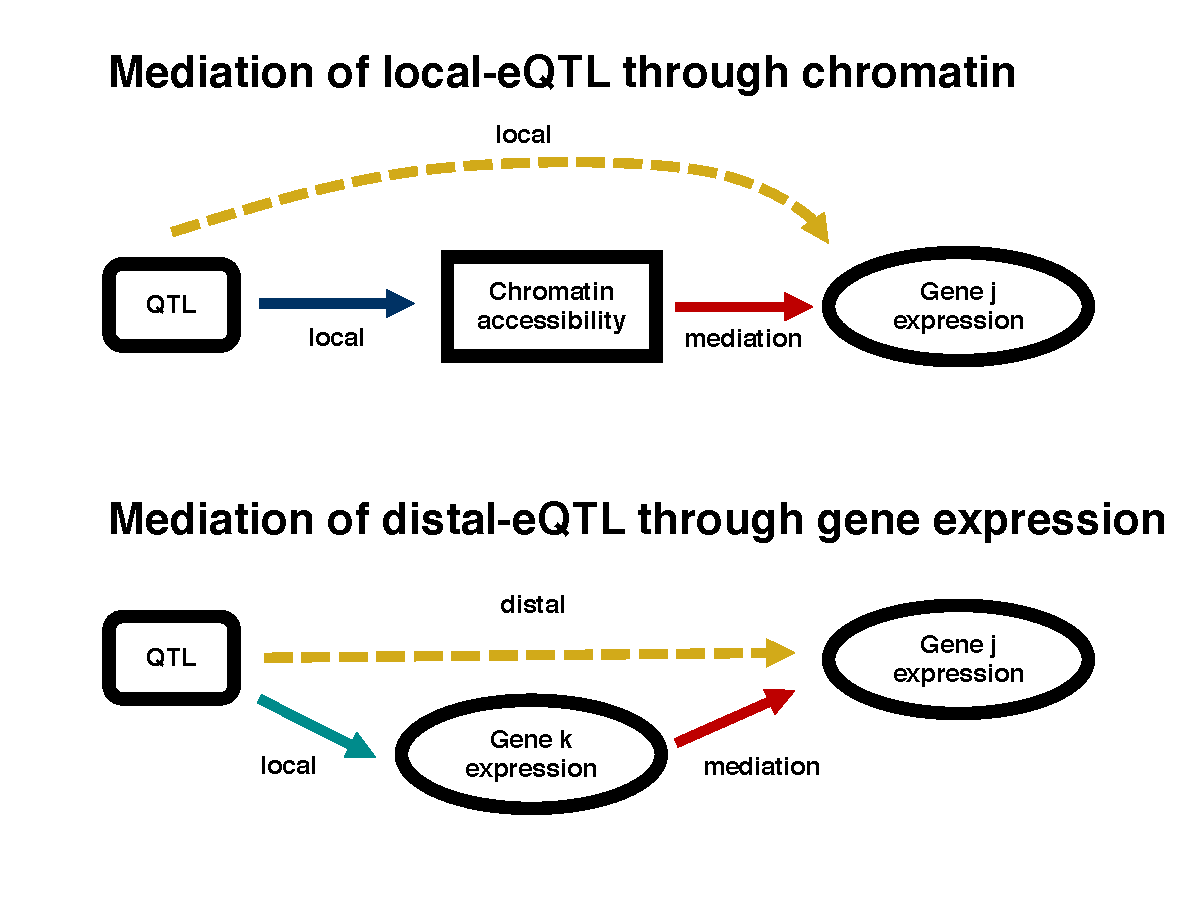
\includegraphics[width=\linewidth, page=1, clip, trim={0in 0.5in 0in 0in}]{figs/mediation_graph.pdf}
\caption{\textbf{Simple mediation models for the genetic regulation of gene expression.} The top model is the mediation of local-eQTL through chromatin accessibility in the region of the gene. This model of mediation is consistent with genetic variation influencing the accessibility of gene j to the transcriptional machinery. The bottom model represents distal-eQTL that are mediated through the transcription of genes proximal to the QTL. Mediation through proximal gene expression is consistent with distal-eQTL that result from as transcription factor activity. \label{fig:graph}}
\end{figure}

\subsubsection{Genome-wide mediation.}

Mediation analysis have recently been used with genomic data, including in humans (\eg \citealt{Battle2014}). We use a similar approach to \cite{Chick2016} and \cite{Keller2018} to assess statistically significant mediation of eQTL effects on gene expression.

The mediation relationships are evaluated in a genome-wide  scan, allowing for the detection of FWER-corrected significant mediators that satisfy relationships \ref{rel:eQTL}, \ref{rel:cQTL}, and \ref{rel:full_mediator}. Similar to the QTL mapping genome scan described in Eq \ref{eq:alternative_model} and Eq \ref{eq:conditional_model}, the mediation scan involves a comparison of an alternative and a null model at loci across the genome. The alternative model is
\begin{equation}
y^{\text{G}_{j}}_{i} = \mu + \text{eQTL}_{i}^{\text{G}_{j}} + m_{ik} + \text{batch}_{i} + \varepsilon_{i},
\label{eq:mediation_alt}
\end{equation}
which is compared to the null model:
\begin{equation}
y^{\text{G}_{j}}_{i} = \mu + m_{ik} \nonumber + \text{batch}_{i} + \varepsilon_{i}
\label{eq:mediation_null}
\end{equation}
where $y^{\text{G}_{j}}_{i}$ is the expression levels for individual $i$ of gene $j$ with an eQTL, $\mu$ is the intercept term, $\text{eQTL}_{i}^{\text{G}_{j}}$ is the eQTL effect on gene $j$, $m_{ik}$ is the effect of the $k$\textsuperscript{th} mediator, either chromatin accessibility or gene expression depending on the mediation model being evaluated, $\text{batch}_{i}$ is the effect of the sequencing center, and $\varepsilon_{i}$ is random noise. Conditioned loci can be included for certain eQTL, as in Eq \ref{eq:conditional_model}, but not included here for clarity. Whereas with the QTL genome scan, the locus effect was changed at each position, for the mediation scan, it is fixed at the eQTL locus, and the mediator is changed.

Because the eQTL is always included in the alternative model but not the null model, the logP of the mediation scan should fluctuate around the observed eQTL logP. At mediators that possess some or all of the information present in the eQTL, the logP will drop. Significant logP drops represent candidate mediators. Significance thresholds to control FWER were determined by performing mediation scans on 1,000 permutations of the mediator variable. See \textbf{Appendix C} for greater detail on the mediation analysis, including permutation approach to significance thresholds and the formal criterion for mediation detection.



\subsection{Software and Data Availability}

All statistical analyses were conducted with the R statistical programming language \citep{RSoftware2018}. The R package miQTL was used for all the mapping and mediations analyses, and is available on GitHub at \url{https://github.com/gkeele/miqtl}. A static version of miQTL is also provided in the \textbf{Supplement} (File S1).

\section{Results}

\subsection{Tissue-specific genome-wide gene expression and chromatin accessibility in three tissues}

Gene expression, using RNA-seq, and chromatin accessibility, using ATAC-seq, were measured in lung, liver, and kidney tissues of 47 unique strains in the Collaborative Cross (CC) mouse population. As the function of each tissue is quite distinct, we expected that these data would reflect tissue-specific differences. Principal components analysis (PCA) on each of the gene expression and chromatin accessibility profiles clearly show the clustering of all samples by tissue (\textbf{Figure \ref{fig:pca_plots}}). 

To further validate the quality of these data, we performed pairwise differential expression (DE) and differentially accessible region (DAR) analysis between the three tissues (\textbf{Table \ref{tab:diff_gene}}). We found between 3,564-5,709 DE genes, and 28,048-40,797 DARs across the comparisons (FWER < 0.1). For both expression and chromatin accessibility, liver and kidney tissues were the most similar, and lung and liver were the most distinct, also reflected in the PCA plots. Pathway analyses show many between-tissue differences related to metabolic and immune-related pathways (Supplementary File 1; FWER < 0.1) that reflects the distinct demands of each tissue. Energy metabolism pathways were more active in liver and kidney and immune-related pathways were more pronounced in lung. We compared the concordance between DE genes and DARs genome-wide and observed that most DE gene promoters do not show significant differences in chromatin accessibility (\textbf{Figure \ref{fig:diff_concordance}}). However, in cases where there is significantly variable accessibility in the promoter of a DE gene, the vast majority agree in direction (i.e. higher expression and greater accessibility). Together, these results support the high quality of the gene expression and chromatin accessibility data.

\begin{figure*}[h]
\renewcommand{\familydefault}{\sfdefault}\normalfont
\centering
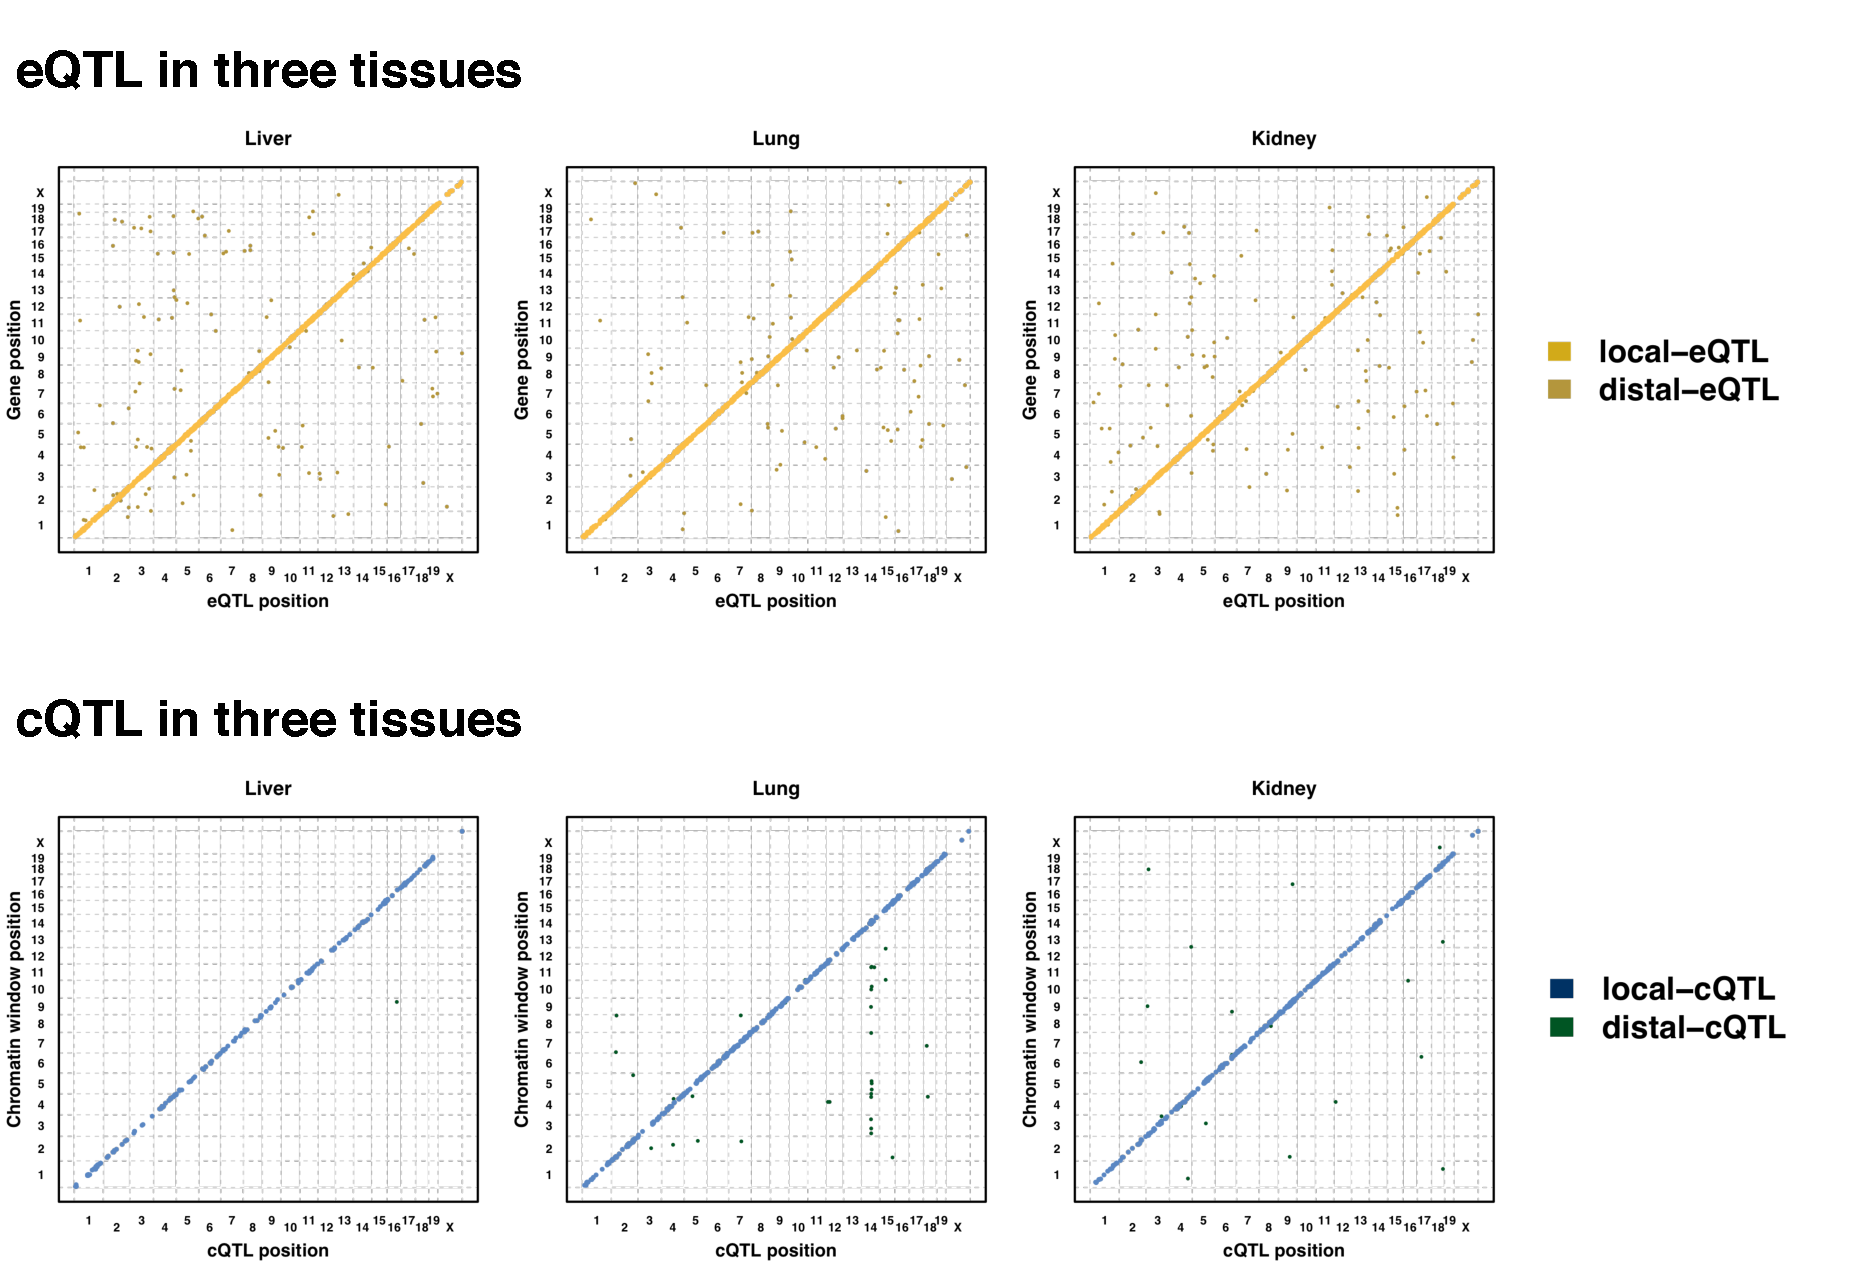
\includegraphics[width=\textwidth, trim={0in 0in 0in 0in}, clip]{figs/qtl_map_main.pdf}
\caption{\textbf{Detected QTL are largely local for both gene expression and chromatin accessibility.} Detected QTL from Method 1 (multi-stage FDR) and Method 3 (genome-wide and chromosome-wide) are included, excluding intra-chromosomal distal-QTL detected through Method 2. The y-axis represents the genomic position of the gene or chromatin site, and the x-axis represents the genomic position of the QTL. Local-QTL appear as dots along the diagonal, and distal-QTL off of it.
\label{fig:grid_plot}}
\end{figure*}

\subsection{Tissue-specific expression QTL}

To evaluate the impact of genetic variation on gene expression, three approaches to detect eQTL were used (\textbf{Table \ref{tab:qtl_procedures}}), summarized here and described more completely in \textbf{Appendix B}. Method 1 was the most stringent and involved a multi-stage conditional regression procedure paired with an FDR control that allowed for the detection of potentially multiple eQTL per gene and requiring significance at a genome-wide level. Method 2 required FDR-controlled significance at the less stringent chromosome-wide level and only used results from the first stage of the multi-stage analysis, which we refer to as a single-step analysis. Method 3 was also a single-step analysis and employed an even more lenient significance criteria based on the genome-wide and chromosome-wide adjusted FWER p-value. We classified local-eQTL as being within 10 Mb of the transcription start site (TSS) of the gene, and distal-eQTL as being greater than 10 Mb from the TSS on the same chromosome (intra-chromosomal) or on a different chromosome (inter-chromosomal). For Method 2, only local-eQTL and intra-chromosomal distal-eQTL were detected due to our use of chromosome-wide significance criteria. For Method 3, the least stringent method, we only detected local-eQTL.

After filtering lowly expressed genes, a total of 8401, 11357, and 10092 genes were considered for liver, lung, and kidney tissues, respectively; a breakdown of the genes analyzed per tissue for QTL analysis is provided in \textbf{Figure \ref{upset_genes_chromatin} [left]} using an UpSet plot \citep{Conway2017}. Positions of local-eQTL detected for each tissue using any of the three methods (Method 1, genome-wide q-value < 0.1; Method 2, chromosome-wide q-value < 0.1; Method 3, genome-wide and chromosome-wide FWER p-value < 0.05)  are shown in \textbf{Figure \ref{fig:grid_plot} [top]} (light colored dots), as well as summarized in \textbf{Table \ref{tab:eqtl_mapping}}. We also identified eQTL with Method 1 using a more relaxed significance threshold (q-value < 0.2; \textbf{Table \ref{tab:eqtl_mapping_lenient}}). Increasing the FDR threshold from 0.1 to 0.2 increases the number of distal-eQTL detected to a greater extent than local-eQTL. Using Method 3 and requiring genome-wide significance, the percentage of tested genes with local-eQTL are 6.3\%, 8.4\%, and 9.5\% for lung, liver, and kidney, respectively (\textbf{Table \ref{tab:eqtl_mapping}}). These percentages increase to 16.6\%, 19.8\%, and 20.8\% when criteria were less stringent with only chromosome-wide significance. The majority of genes with local-eQTL were only observed in one tissue (\textbf{Figure \ref{fig:upset_eqtl_cqtl} [left]}).

For each eQTL detected by any of our methods, we estimated the effect size of the eQTL by two methods (see \textbf{Tables XX}), either the coefficient of determination ($R^{2}$) for the fixed effect fitting of the QTL term (\textbf{Methods}; Eq \ref{eq:effect_size}) or as the proportion of variance explained based on the variance component estimate from a random effect fitting of the QTL term (\textbf{Methods}; Eq \ref{eq:effect_size_ranef}). We primarily report results from the fixed effect approach because the estimates were largely consistent with plausible QTL effect sizes given the size of the study, outlined in \cite{KeeleSPARCC}, namely we were not well-powered to detect QTL with effect sizes < 50\% at genome-wide significance. As expected, Method 1 detects eQTL with large effects (\textbf{Figure \ref{fig:qtl_effect_sizes_by_method}}, red dots). The less stringent Methods 2 and 3 result in greater power to detect local-eQTL with reduced effects (\textbf{Figure \ref{fig:qtl_effect_sizes_by_method}}, gray and blue dots). Distal-eQTL discovered with the multi-stage mapping procedure (Method 1; q-value < 0.1) were detected for $\leq$ 1.6\% of tested genes (\textbf{Table \ref{tab:eqtl_mapping}}; \textbf{Figure \ref{fig:grid_plot} [top]}, dark colored dots), and, consistent with previous studies (\textit{eg} \citealt{Chick2016}), have weaker effects than local-eQTL (\textbf{Figure \ref{fig:qtl_effect_sizes_strict} [top]}). For both Methods 1 and 2, almost three times as many local-eQTL are detected compared to distal-eQTL, likely reflecting these stronger effects. For some distal-eQTL, the effect sizes estimated through random effects models approach zero, potentially resulting from highly influential data points in the fixed effect regression procedure and are thus likely to be false positives (\textbf{Figure \ref{fig:qtl_effect_size_fixefvsranef}}). 

To assess whether distance measures to classify intra-chromosomal local- vs distal-eQTL were reasonable, we plotted the statistical association for all intra-chromosomal eQTL from Method 1 (\textbf{Figure \ref{fig:genomewide_dist} [top]}) and the less stringent Method 2 (\textbf{Figure \ref{fig:chrwide_dist} [top]}). In addition to finding that the majority are local-eQTL, we see a drastic reduction in the strength of the statistical association outside of the defined local region. This suggests that intra-chromosomal distal-eQTL are more similar to inter-chromosomal distal-eQTL than local-eQTL, and that our 10Mb boundaries are appropriate. 

Founder allele effects were estimated for all eQTL, using a random effects model to constrain unstable estimates. Consistent with previous studies (\eg \citealt{Aylor2011}), the CAST and PWK alleles tended to have more extreme effects than the classical inbred strains. This pattern was observed for both local and distal eQTL (\textbf{Figure \ref{fig:eqtl_effects_abs}}).

\subsection{Tissue-specific chromatin QTL}

To determine genetic effects on chromatin structure, genomic regions were divided into $\sim$300 base pair windows, and used in chromatin accessibility QTL (cQTL) analysis with the same methods used for eQTL. We tested 11448, 24426, and 17918 chromatin regions in liver, lung, and kidney, respectively. The overlap in chromatin windows across tissues is described in \textbf{Figure \ref{fig:upset_genes_chromatin} [right]}. Overall, there were substantially fewer cQTL detected compared to eQTL for all tissues (\textbf{Figure \ref{fig:grid_plot} [bottom]};\textbf{Table \ref{tab:cqtl_mapping}}). As with eQTL, cQTL are more likely to be local (66\%-94.1\% for Method 1; 75\%-90\% for Method 2).
Consistent with eQTL, the effect sizes of local-cQTL are on average higher than distal-cQTL (\textbf{Figure \ref{fig:qtl_effect_sizes_strict} [bottom]}), likely contributing to the to the small number of detected distal-cQTL. cQTL with low effect size are primarily distal-cQTL and may represent false positives. Likewise, most intra-chromosomal cQTL detected using Method 1 or 2 are local-cQTL, and the significance of association is much greater for the local-cQTL  (\textbf{Figure \ref{fig:genomewide_dist} [bottom]} and \textbf{Figure \ref{fig:chrwide_dist} [bottom]}). Similar to local-eQTL, though to a lesser extent, the majority of chromatin windows with local-cQTL were only observed in one tissue (\textbf{Figure \ref{fig:upset_eqtl_cqtl} [right]}).
Again we found that the CAST and PWK founder alleles have more extreme effects than the other strains for local-cQTL, though the pattern is less pronounced than with local-eQTL, likely due to the reduced number of cQTL (\textbf{Figure \ref{fig:cqtl_effects_abs}}). The numbers of detected distal-cQTL are low, and no clear trends are obvious.

\section{Paired QTL detected in multiple tissues}

For a given trait, QTL from different tissues were paired based on co-localizing to approximately the same genomic region. For local-QTL, both had to be within the local window, defined at 10 Mb around the gene TSS, resulting in a maximum distance of 20 Mb between QTL. For distal-eQTL, both had to be within 10 Mb of each other. 
For local-eQTL, 761 (liver/lung), 1206 (liver/kidney), and 1025 (lung/kidney) pairs were detected. With distal-eQTL, 61 (liver/lung), 120 (liver/kidney), and 59 (lung/kidney) were identified. For cQTL, the vast majority of pairs were local, with 55 (liver/lung), 56 (liver/kidney), and 142 (lung/kidney). Only 4 distal-cQTL pairs were observed, all between lung and kidney. The effect sizes of paired QTL vary across tissues, though they were significantly correlated (\textbf{Figure \ref{fig:qtl_effect_size_comparison}}).

Correlations between the founder allele effects for pairs of QTL were calculated (FDR $\le 0.1$; \textbf{Figures \ref{fig:qtl_pair_histograms}}), with 345 (liver/lung), 623 (liver/kidney), and 498 (lung/kidney) local-eQTL pairs and 21 (liver/lung), 34 (liver/kidney), and 16 (lung/kidney) distal-eQTL pairs positively correlated. Highly correlated QTL pairs were highly proximal to each other (\textbf{Figure \ref{fig:qtl_cor_by_distance_comparison}}), suggesting that the underlying causal variants are the same or linked. 47 (liver/lung), 48 (liver/kidney), and 118 (lung/kidney) positively correlated local-cQTL pairs. The correlations between distal-cQTLs were not formally tested because there were only four pairs; however, three of the four pairs had correlations greater than 0.5. No negatively correlated QTL pairs were detected, after accounting for multiple testing.

\begin{figure*}[h!]
\renewcommand{\familydefault}{\sfdefault}\normalfont
\centering
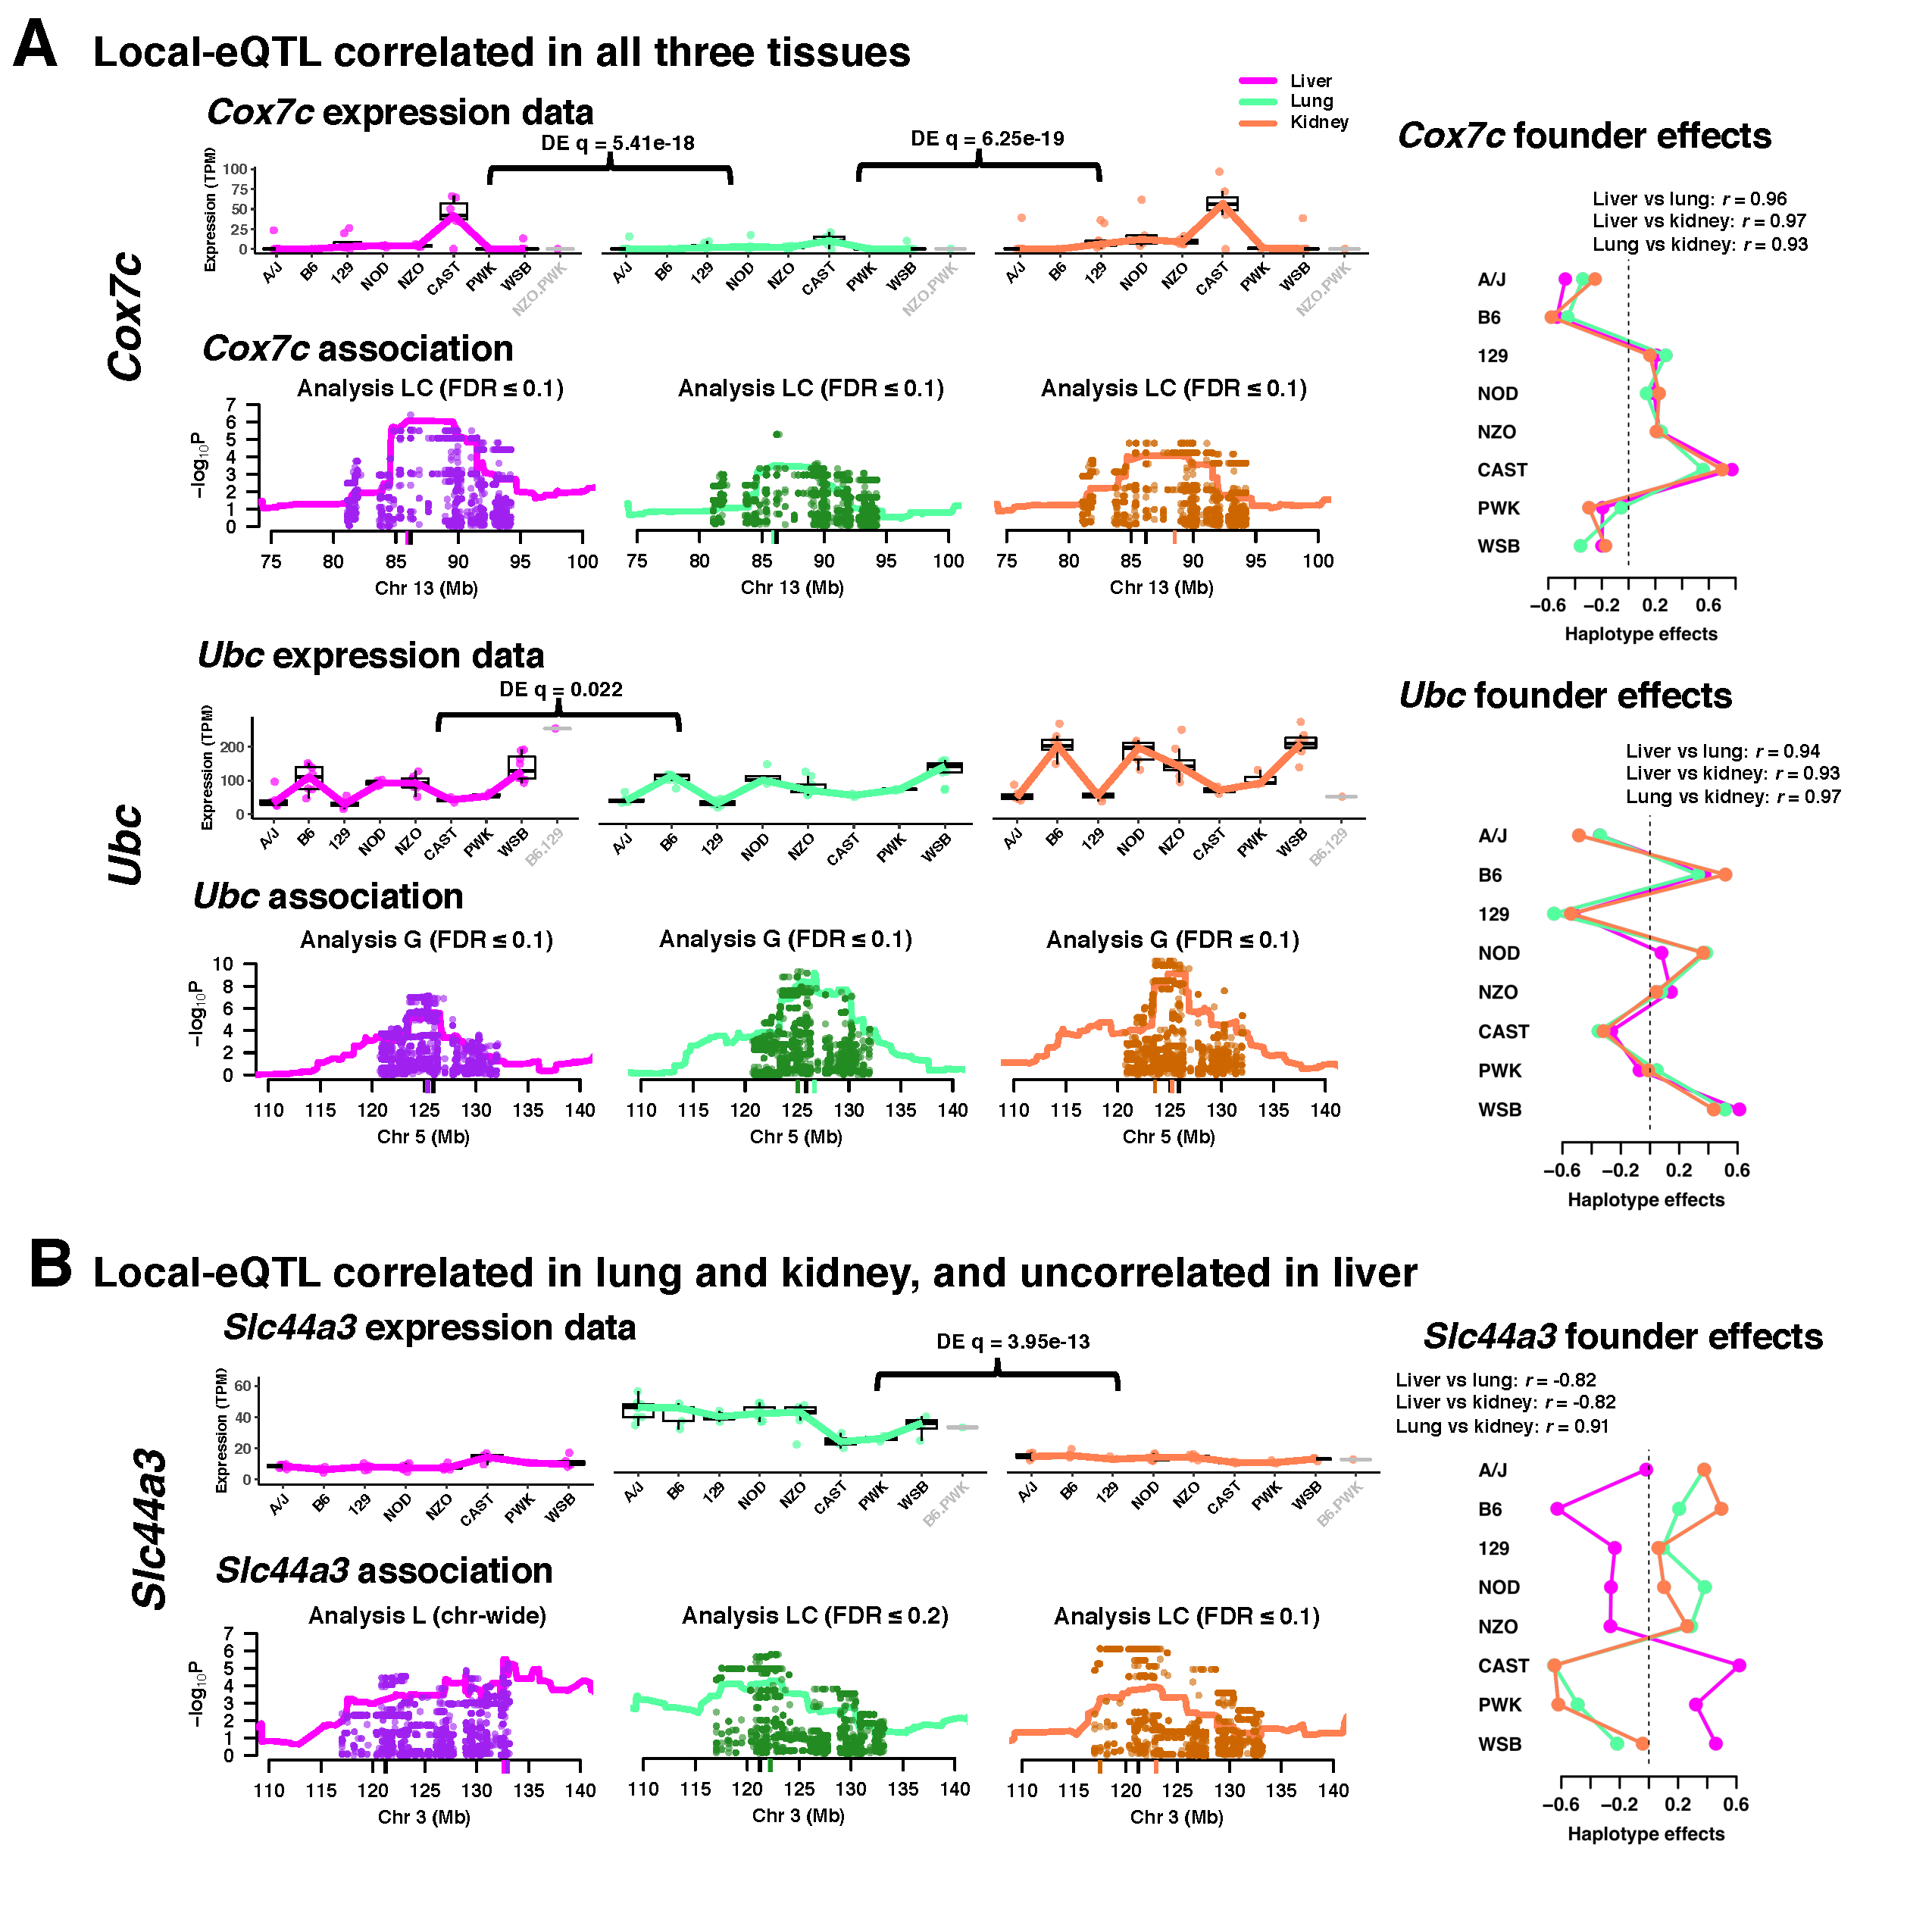
\includegraphics[width=0.9\textwidth, trim={0in 0.5in 0in 0in}, clip]{figs/correlated_local_eqtl.pdf}
\caption{\textbf{Examples of genes with local-eQTL observed in all three tissues.} \textit{Cox7c} and \textit{Ubc} possess local-eQTL with highly correlated founder alllele effects across all three tissues, supportive of shared causal origin (A). \textit{Slc44a3} has a more complicated pattern of local-eQTL founder effects across the tissues, with correlated effects shared between lung and kidney, and transgressive effects in the liver eQTL by comparison, consistent with distinct casual variants comparing liver to lung and kidney. (B). For each gene, the expression data is plotted with boxplots based on most likely founder haplotype pair (diplotype), and differential expression between tissues is highlighted. The haplotype association for each tissue is also included near the gene TSS with variant association overlaid. The most statistically rigorous method to detect the QTL is also included. The black tick represents the gene TSS and the colored ticks represent haplotype and variant peaks. Founder effects estimated as constrained BLUPs are also included with their pairwise correlations. Estimated effects were generally consistent with the expression data.\label{fig:correlated_local_eqtl}}
\end{figure*}

%\subsection{Genes with correlated local-eQTL: \textit{Cox7c} and \textit{Ubc}}

Cytochrome c oxidase subunit 7C (\textit{Cox7c}) and ubiquitin C (\textit{Ubc}) are examples of genes that possess local-eQTL with highly correlated effects in all three tissues (\textbf{Figure \ref{fig:correlated_local_eqtl}A}).
For \textit{Cox7c} local-eQTL were driven by high expression when the CAST allele was present, intermediate expression with 129, NOD, and NZO alleles, and low expression with A/J, B6, PWK, and WSB alleles. The \textit{Ubc} local-eQTL were driven by high expression with the B6, NOD, NZO, and WSB alleles. Though the founder effects are consistent across tissues for both genes, we note that expression of \textit{Cox7c} was significantly higher in liver compared to both lung ($q = \num{5.41e-18}$) and kidney ($q = \num{6.25e-19}$), and for \textit{Ubc}, expression in liver and lung were considered significantly differential ($q = 0.022$). 

%The haplotype and variant associations in the local region match closely for all tissues for both \textit{Cox7c} and \textit{Ubc}. Though all the \textit{Ubc} local-eQTL were detected with the most stringent Method 1, the \textit{Cox7c} local-eQTL were detected with the more lenient Method 2.

%\subsection{Genes with uncorrelated local-eQTL: \textit{Slc44a3} and \textit{Pik3c2g}}

\begin{figure*}[h]
\renewcommand{\familydefault}{\sfdefault}\normalfont
\centering
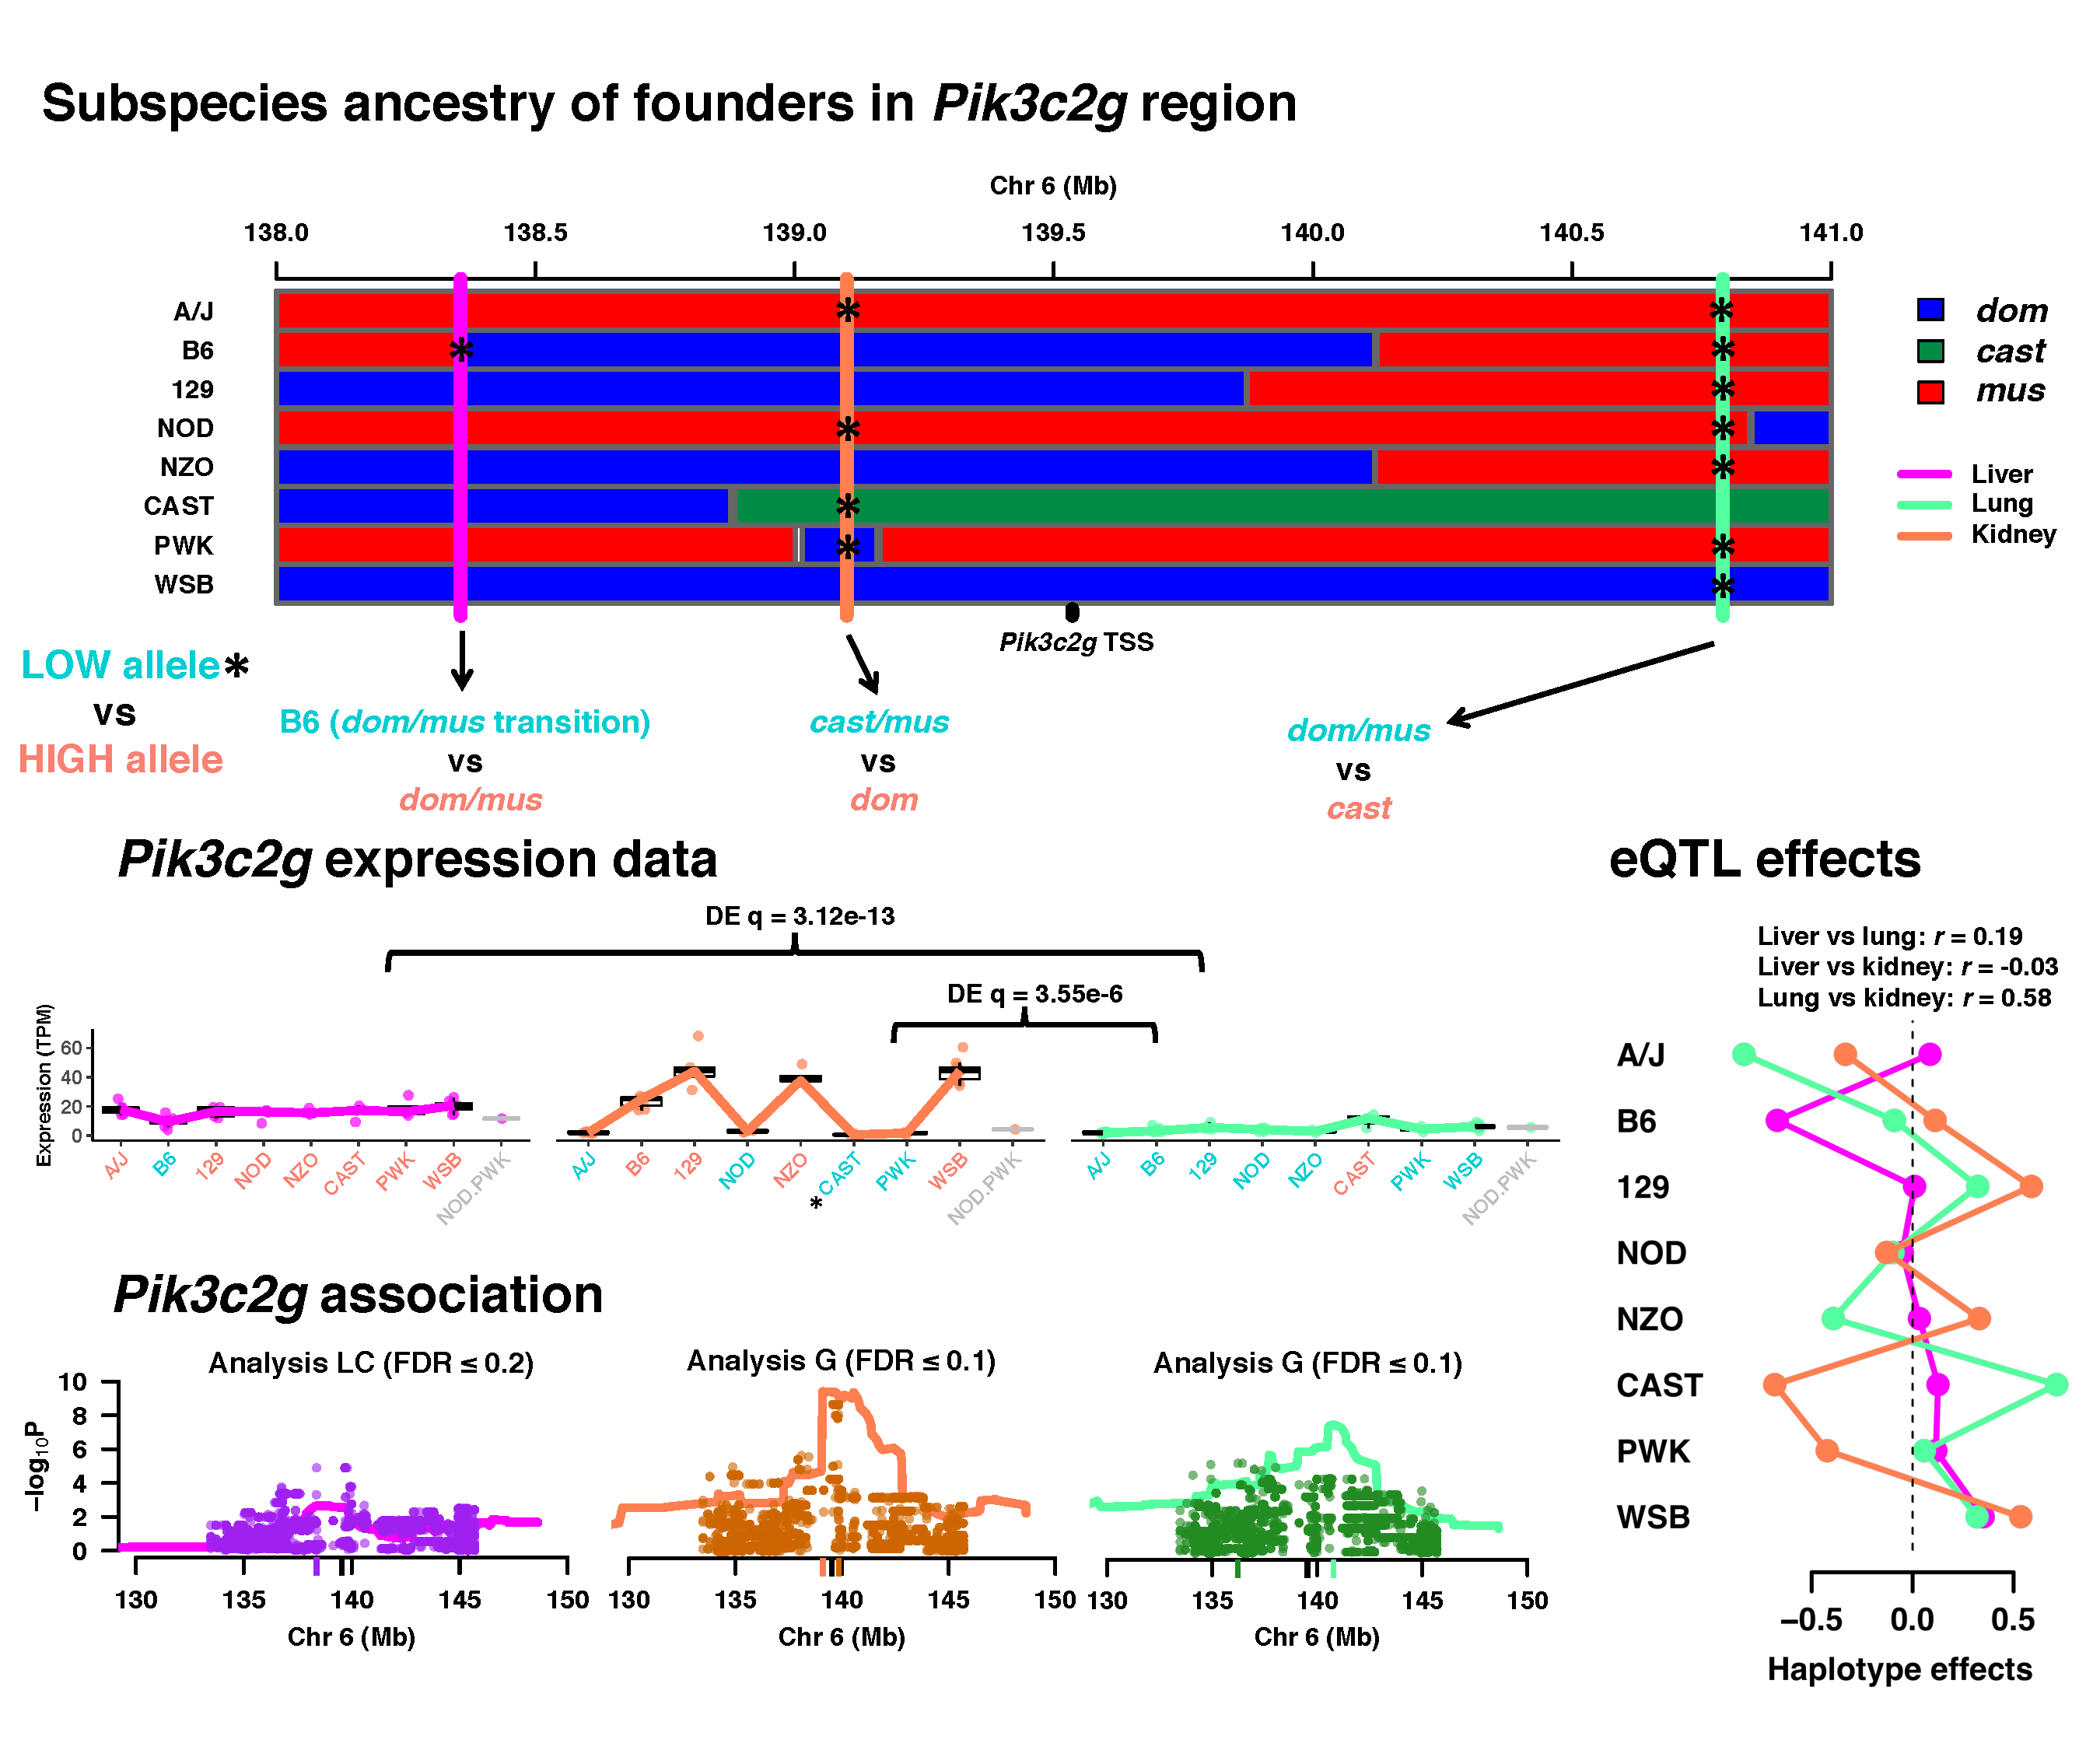
\includegraphics[width=0.9\textwidth, trim={0in 0.5in 0in 0in}, clip]{figs/pik3c2g_example.pdf}
\caption{\textbf{\textit{Pik3c2g} possesses tissue-specific local-eQTL.} Local-eQTL for \textit{Pik3c2g} are detected in all three tissues in the 3Mb region surrounding its TSS. The genomes of the CC founders can be simplified in terms of contributions from three subspecies lineages of \textit{M. musculus}: \textit{dom} (blue), \textit{cast} (green), and \textit{mus} (red). The effects of each local-eQTL matched the subspecies contributions near the eQTL coordinates, with low subspecies alleles colored teal and high alleles colored salmon, consistent with local-eQTL for \textit{Pik3c2g} being distinct and tissue-specific. The gene expression data is represented as boxplots, categorized based on most likely diplotype at the eQTL for each CC strain. Haplotype and variants associations are included for each tissue, with the black tick representing the \textit{Pik3c2g} TSS and colored ticks representing haplotype and variant peaks. The most rigorous procedure to detect each QTL is reported. Founder effects, estimated as constrained BLUPs, were consistent with the expression data, and uncorrelated across the tissues.\label{fig:pik3c2g}}
\end{figure*}

QTL pairs that are uncorrelated potentially represent distinct tissue-specific QTL where genetic variants influence gene expression or chromatin accessibility in a tissue-specific pattern. For example, the solute carrier family 44, member 3 (\textit{Slc44a3}) gene has correlated local-eQTL effects in lung and kidney, but unique effects in liver (\textbf{Figure \ref{fig:correlated_local_eqtl}B}). Notably, the effects in liver are anti-correlated with the effects in lung and kidney, suggesting the liver eQTL could be transgressive \citep{Rieseberg1999} to the eQTL in lung and kidney, whereby the effects of the founder alleles are reversed. For \textit{Slc44a3}, CAST, PWK, and WSB alleles result in higher expression in liver, but lower expression in lung and kidney. 
The local-eQTL for \textit{Slc44a3} were more similar in location in lung and kidney, whereas the liver eQTL was more distal to the gene TSS. Overall, the expression data, estimated effects, and patterns of association are consistent with lung and kidney sharing a causal local-eQTL, and liver possessing a unique one. 
%The lung eQTL was detected with the highly lenient Method 2 (FDR $\leq$ 0.2) and the kidney eQTL with the less lenient Method 2 (FDR $\leq$ 0.1). The liver eQTL was detected with the lenient Method 3 (chromosome-wide). 

Another example is phosphatidylinositol-4-phosphate 3-kinase catalytic subunit type 2 gamma (\textit{Pik3c2g}), a gene of interest for diabetes-related traits \citep{Braccini2015}. \textit{Pik3c2g} has local-eQTL in all three tissues but that are all uncorrelated (\textbf{Figure \ref{fig:pik3c2g}}). Expression of \textit{Pik3c2g} varies at statistically significant levels for liver versus lung ($q = \num{3.12e-13}$) and lung versus kidney ($q = \num{3.55e-6}$). The presence of tissue-specific local-eQTL is further supported by the \textit{Mus musculus} lineages in the genomic region local to \textit{Pik3c2g}. The CC founder strains all possess contributions from three subspecies of \textit{M. musculus}: \textit{domesticus} (\textit{dom}), \textit{castaneus}, (\textit{cast}), and \textit{musculus} (\textit{mus}) \citep{Yang2011}. \cite{Crowley2015} found that allele-specific gene expression in mice descended from the CC founders often followed patterns that matched the subspecies inheritance at the gene regions.
In lung, the CAST allele, which represents the \textit{cast} subspecies lineage at the locus, results in higher expression, consistent with a \textit{cast} versus \textit{dom}/\textit{mus} allelic series. In kidney, the B6, 129, NZO, and WSB alleles result in higher expression, whereas A/J, NOD, CAST, and PWK alleles show almost no expression, mostly consistent with a \textit{dom} versus \textit{cast}/\textit{mus} allelic series. The PWK founder has a small \textit{dom} haplotype block at the QTL peak in a broader region that is largely \textit{mus}. The expression data are highly consistent with PWK having the \textit{mus} allele, suggesting that the causal variant is located in a nearby region, supported by the variant association. Notably, the B6 allele expression appears intermediate to the other founders that possess \textit{dom} inheritance, representing a potentially multi-allelic QTL that haplotype association can better identify in comparison to bi-allelic variant association. In liver, the B6 allele resulted in lower expression. The B6 founder does not have a unique subspecies lineage at the locus, but instead possesses a recombination event between \textit{dom} and \textit{mus}, potentially disrupting the local regulation specific to each subspecies lineage and explaining the reduced expression.

%\subsection{Genes with distal-QTL observed across tissues: \textit{Akr1e1}, \textit{Per2}, and \textit{Rnf13}}

\begin{figure*}[h!]
\renewcommand{\familydefault}{\sfdefault}\normalfont
\centering
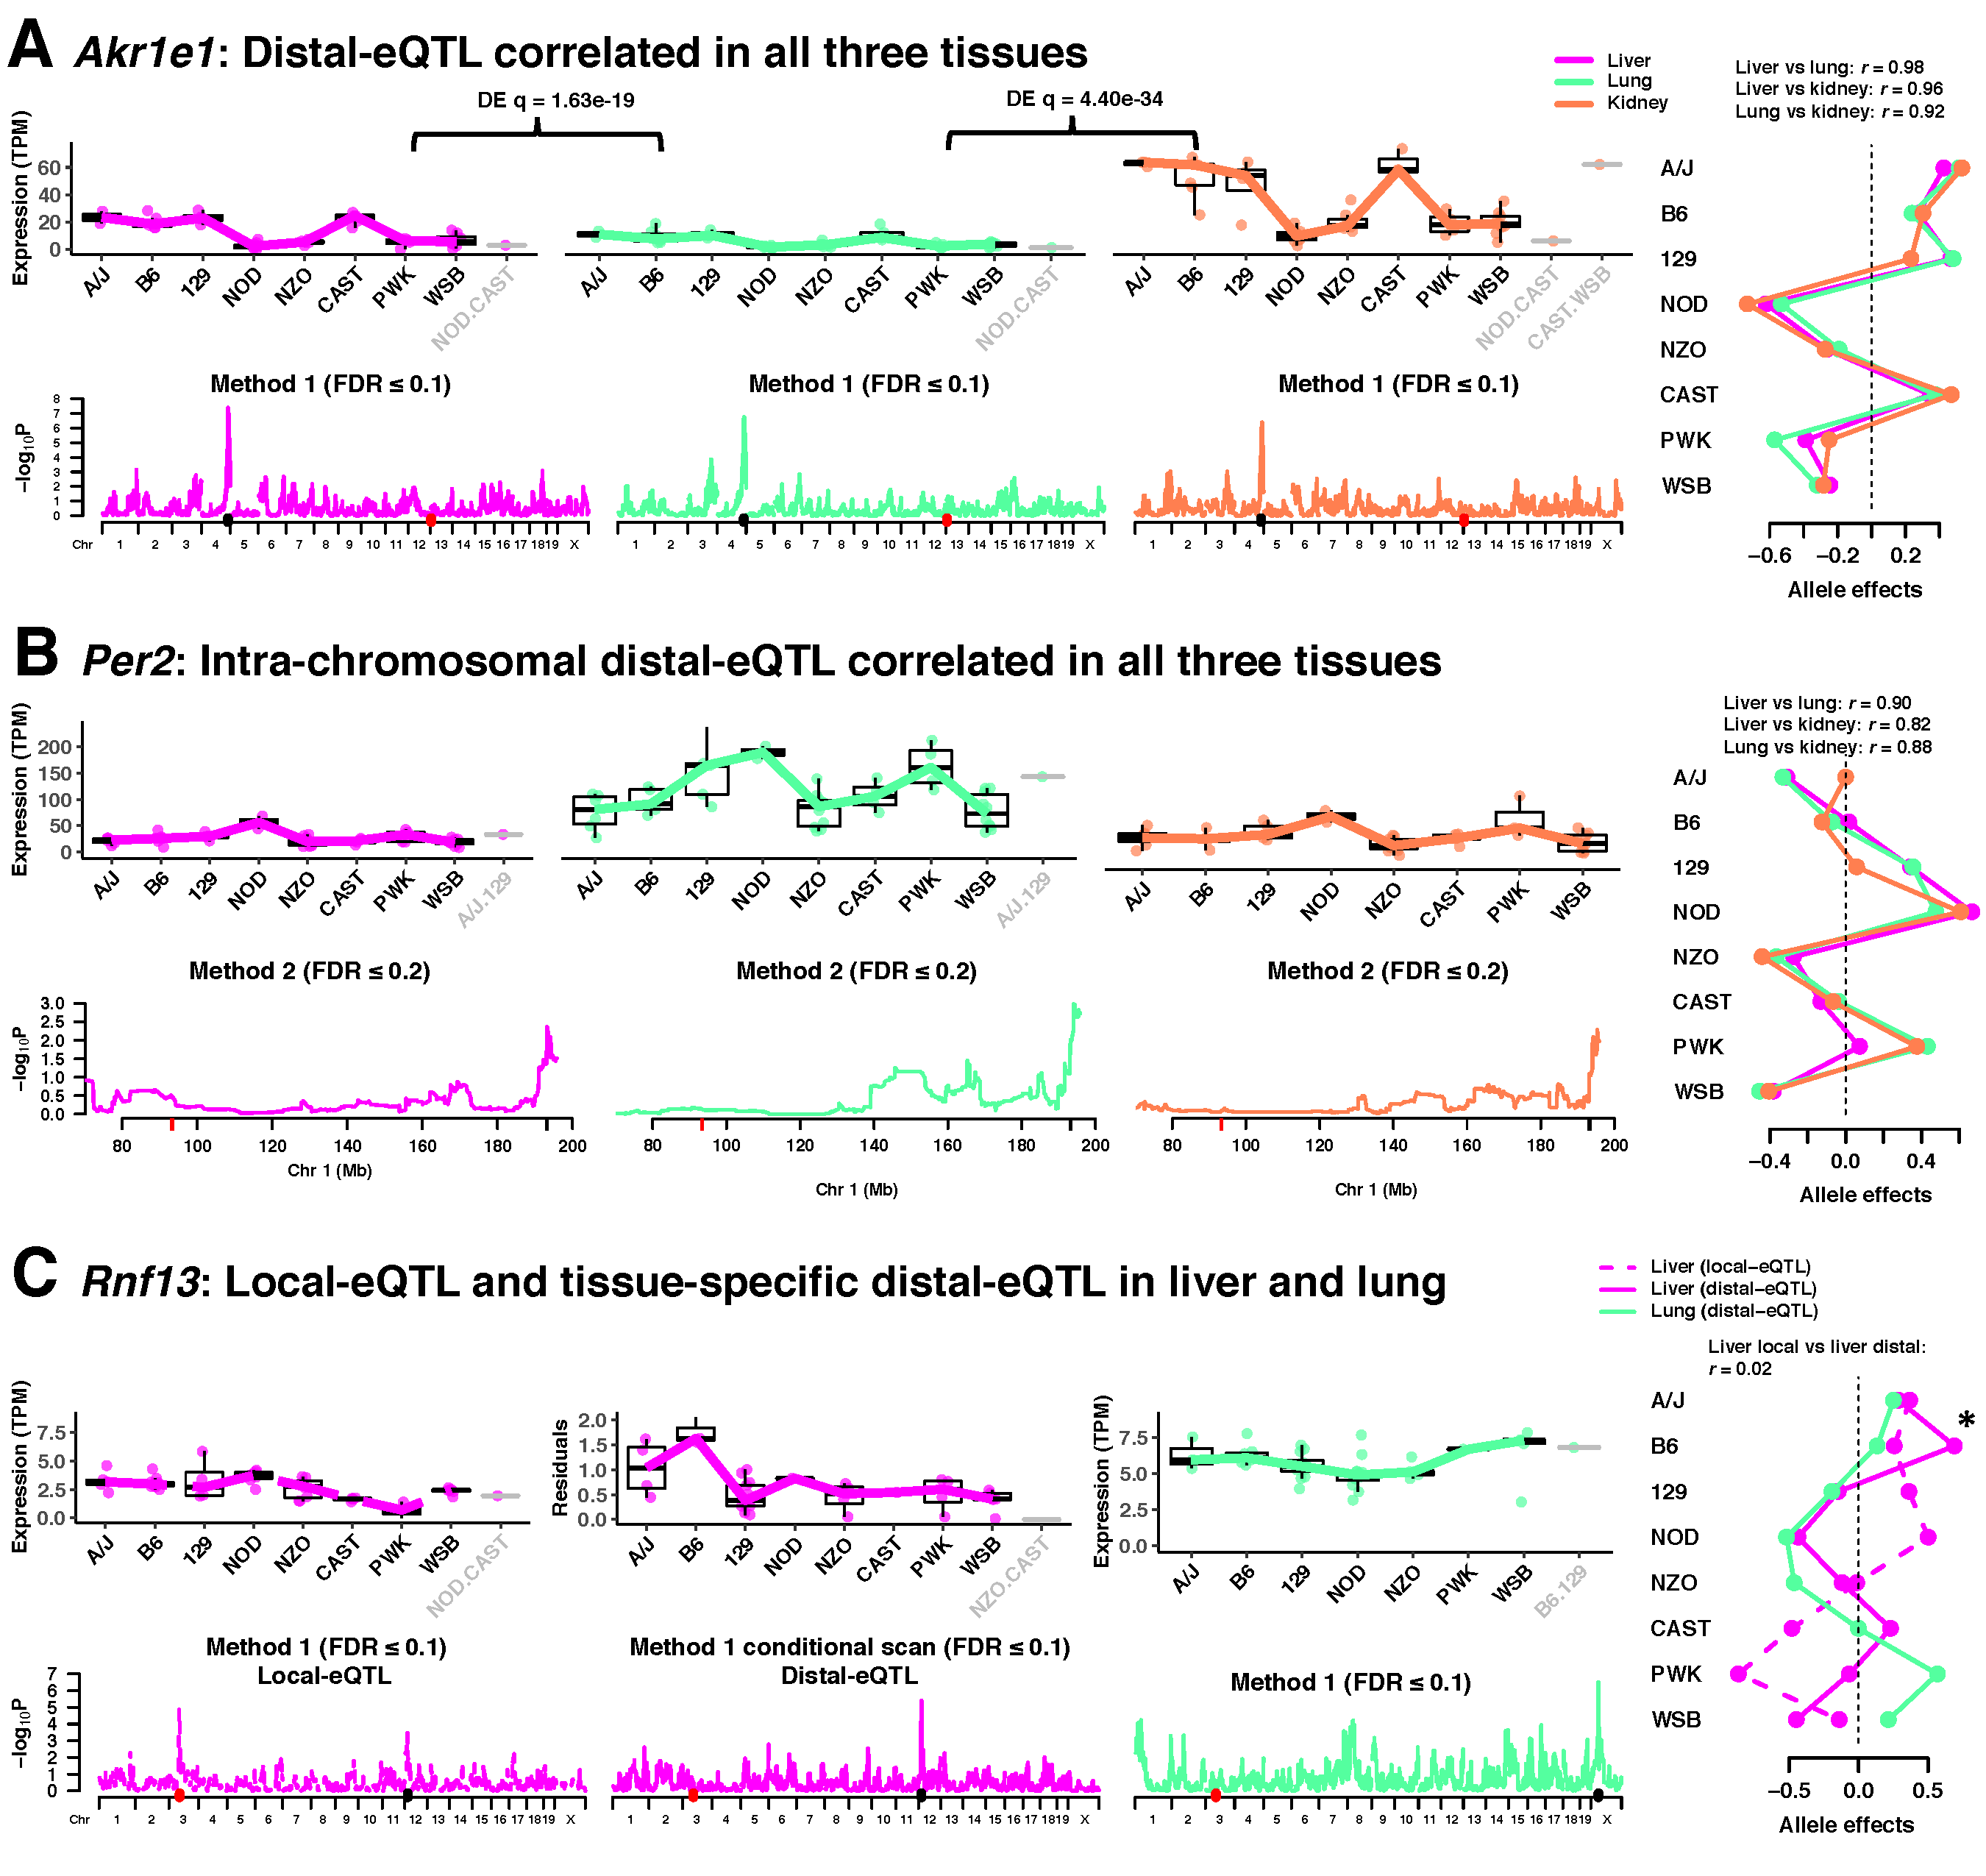
\includegraphics[width=0.9\textwidth, trim={0in 0in 0in 0in}, clip]{figs/correlated_distal_eqtl.pdf}
\caption{\textbf{Examples of genes with distal-eQTL effect patterns across tissues.} \textit{Akr1e1} has highly significant distal-eQTL detected on chromosome 4 in all three tissues with correlated founder effects (A). \textit{Per2} has intra-chromosomal distal-eQTL leniently detected 100Mb away from the TSS, also with highly correlated founder effects across the tissue, providing further support that the distal-eQTL are real (B). \textit{Rnf13} has a liver-specific distal-eQTL on chromosome 12 detected after conditioning on its local-eQTL on chromosome 2, and a lung-specific distal-eQTL on chromosome X, each with distinct founder effect patterns (C). Expression data are represented as boxplots for most likely diplotype, with differential expression noted when significant. Haplotype associations for each tissue distal-eQTL combination are shown, with the most rigorous statistical procedure for detection reported. Red ticks signify the gene TSS and black ticks represent that eQTL peak. Fit founder effects, estimated as BLUPs, are included, along with the pairwise correlations of the eQTL. The black asterisk marks the high B6 effect that drives the distal-eQTL in liver after conditioning on the local-eQTL for \textit{Rnf13}.
\label{fig:correlated_distal_eqtl}}
\end{figure*}

\begin{figure*}[h]
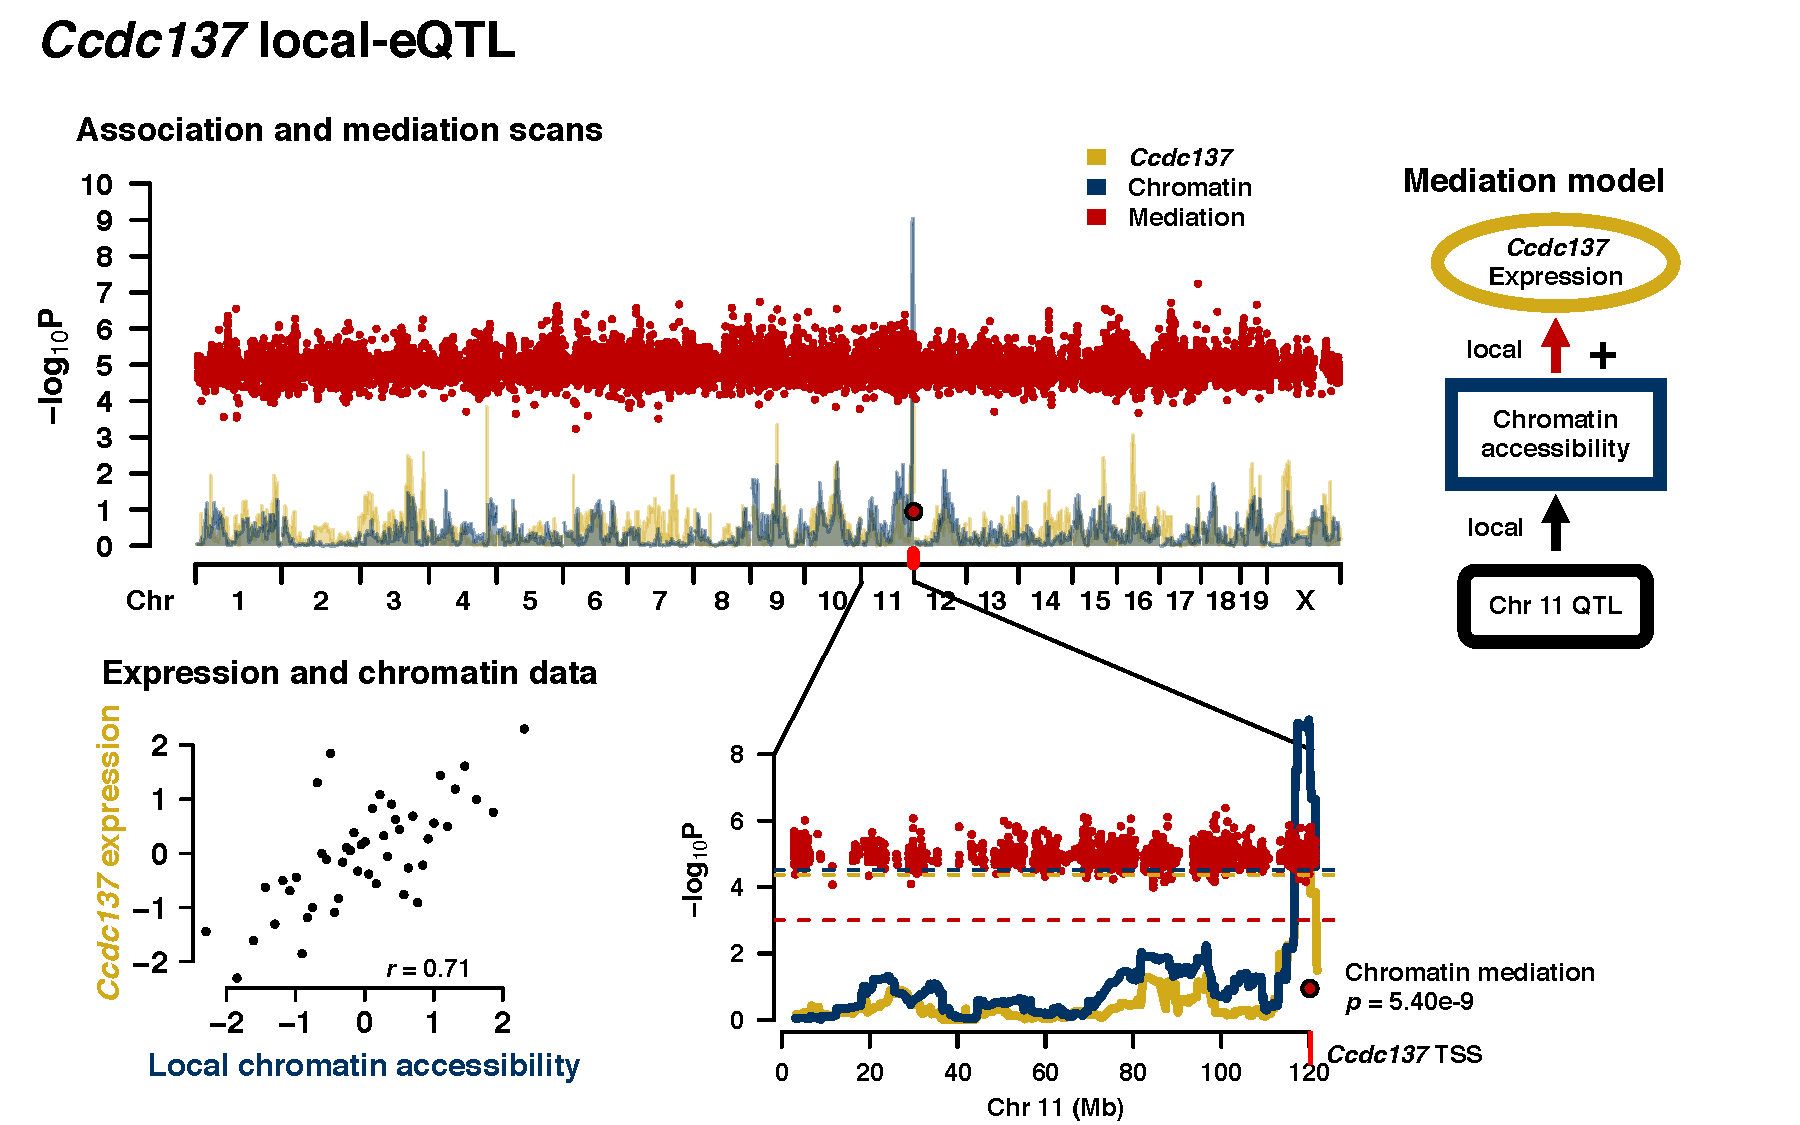
\includegraphics[width=\textwidth, trim={0in 0in 0in 0in}, clip]{figs/ccdc137_mediation.pdf}
\caption{\textbf{\textit{Ccdc137} local-eQTL is mediated by proximal chromatin accessibility.} \textit{Ccdc137} expression and the chromatin accessibility in the proximal region are highly correlated ($r = 0.71$). Genome scans for \textit{Ccdc137} expression (yellow), nearby chromatin accessibility (blue), and chromatin mediation of the \textit{Ccdc137} local-eQTL (red) in lung tissue. The local-eQTL and local-cQTL for the chromatin region at the TSS of \textit{Ccdc137} (red tick) are over-lapping. The steep drop in the statistical association, represented as logP, for the chromatin site in the mediation scan supports chromatin mediation of \textit{Ccdc137} expression, depicted as a simple graph in the topright. The QTL and mediation signals are detected at genome-wide significance. \label{fig:ccdc137_mediation}}
\end{figure*}

Founder allele effects that correlate across tissues can provide stronger confirmation of distal-QTL, even those with marginal significance. 
%Though fewer distal-QTL were significantly correlated across tissues in comparison to local-QTL (71 to 1,466 for eQTL and 2 to 213), potentially reflecting the reduced power to detect distal-QTL in this study, a number of genes were identified with unique patterns of distal-eQTL over the tissues, shown in \textbf{Figure \ref{fig:correlated_distal_eqtl}}.
For example, the Aldo-keto reductase family 1, member E1 (\textit{Akr1e1}; \textbf{Figure \ref{fig:correlated_distal_eqtl}A}) gene is located on chromosome 13 and had no local-eQTL detected in any of the tissues. Distal-eQTL for \textit{Akr1e1} were detected in all tissues that localize to the same distal region of chromosome 4. The founder allele effects of the distal-eQTL are all highly correlated, with A/J, B6, 129, and CAST being the more highly expressed alleles. The overall magnitude of expression varies significantly across the tissues, with liver and kidney having significantly higher expression than lung ($q = \num{1.63e-19}$ and $q = \num{4.40e-34}$, respectively).
%The distal-eQTL for \textit{Akr1e1} will be discussed further with the topic of mediation.
%As with local-QTL, correlated distal-eQTL can provide strong evidence that marginally significant QTL are valid. 
Another example is the Period circadian clock 2 (\textit{Per2}; \textbf{Figure \ref{fig:correlated_distal_eqtl}B}) gene, which possesses intra-chromosomal distal-eQTL that are detected in all three tissues that are approximately 100 Mb away from its TSS. Despite being detected with the highly lenient Method 2 (FDR $\leq$ 0.2), the founder allele effects are significantly correlated among the tissues, characterized by high expression with the NOD and PWK alleles present. Collectively, these findings provide strong validation for the distal-eQTL, which would commonly not be detected.

QTL analysis in multiple tissues also allows for the detection of tissue-specific distal-QTL. The Ring finger protein 13 (\textit{Rnf13}; \textbf{Figure \ref{fig:correlated_distal_eqtl}C}) gene was lowly expressed in all tissue but with a strong local-eQTL detected in liver. The multi-stage conditional regression approach, conditioning on the local-eQTL, detected a distal-eQTL on chromosome 12. Comparing the residuals after regressing out the local-eQTL and founder allele effects suggested that mice with B6 contributions at the distal locus had higher \textit{Rnf13} expression. In lung tissue, a distal-eQTL was detected on the X chromosome with a different founder allele pattern, notably high expression when A/J, B6, and PWK alleles were present, and low expression with NOD and NZO alleles. These examples demonstrate that analyzing multiple tissues can provide greater evidence of distal-QTL, as well as potentially identify tissue-specific genetic regulation.

\section{Mediation of eQTL}

Measurement of gene expression and chromatin accessibility data in the same mice and tissues enables the use of mediation analysis to elucidate the relationships between genotype, chromatin accessibility, and gene expressions. We assessed evidence for two mediation models of eQTL effects (\textbf{Figure \ref{fig:graph}}). First, we tested for proximal chromatin state as a mediator of the effect of local-eQTL on gene expression using an approach adapted from \cite{Chick2016} to detect mediation through chromatin accessibility of local-eQTL detected through Method 3 (genome-wide and chromosome-wide; see \textbf{Appendix C} for greater detail).  

%\subsection{Mediation of local-eQTL effects through proximal chromatin accessibility}

We found 13-42 local-eQTL showed evidence of mediation through proximal chromatin accessibility at genome-wide significance, and 35-106 at chromosome-wide significance (\textbf{Table \ref{tab:mediation}}). The coiled-coil domain containing 137 gene (\textit{Ccdc137}) is a strong example of mediation through local chromatin accessibility. \textbf{Figure \ref{fig:ccdc137_mediation}} includes the genome scans that identify local-QTL for \textit{Ccdc137} expression (eQTL) and a proximal chromatin accessibility window (cQTL). The red tick marks the TSS for \textit{Ccdc137}, which is highly proximal to both the eQTL and cQTL. The red dots represent the significance of the eQTL after conditioning on each chromatin region as a mediator. A large drop in eQTL significance at the location of the cQTL represents a strong mediation signal. A closer inspection of the region shows that the significance of the eQTL and cQTL are similar but notably stronger for chromatin, as expected by the proposed mediator model. 

Co-localization of eQTL and cQTL is not sufficient for mediation, shown in \textbf{Figure \ref{fig:colocalization}}. For both \textit{Hdhd3} in liver (\textbf{Figure \ref{fig:colocalization} [left]}) and the acyl-Coenzyme A binding domain containing 4 gene (\textit{Acbd4}) in kidney (\textbf{Figure \ref{fig:colocalization} [right]}), there are local-eQTL with a co-localizing cQTL. Comparing the statistical associations at the genomic locations of the eQTL and cQTL as well as the founder haplotype effects for both the eQTL and cQTL, the correspondence in both is better for \textit{Hdhd3} compared to \textit{Acbd4}. As with \textit{Ccdc137}, a strong mediation signal is detected for \textit{Hdhd3}, indicated by the decrease in the eQTL association when conditioning on the chromatin state. Mediation is not detected for \textit{Abcd4}, which is consistent with the genetic regulation of both gene and chromatin site not stemming from the same causal origin.

%\subsection{Mediation of distal-eQTL effects through proximal gene expression}

Next, we tested for evidence of expression levels of genes proximal to distal-eQTL acting as mediators, using an approach similar to \cite{Keller2018} for distal-eQTL detected through Method 1. 
%A related mediation model was used to identify genome-wide significant distal-eQTL that are mediated through the expression of proximal genes, as might be expected for a transcription factor with its own local-eQTL (\textbf{Figure \ref{fig:graph} B}). 
Eight genes were identified with mediated distal-eQTL (\textbf{Table \ref{tab:exmediation}}). As example, the distal-eQTL of cyclin Y-like 1 (\textit{Ccnyl1}) is mediated by the expression of zinc finger protein 979 (\textit{Zfp979}), a putative transcription factor (\textbf{Figure \ref{fig:ccnyl1_exmediation}}). The founder haplotype effects at the distal-eQTL of \textit{Ccnyl1} are highly correlated with the local-eQTL effects for \textit{Zfp979}, though with a reduction in overall strength, in accordance with the proposed mediation model.

\begin{figure*}[hp]
\renewcommand{\familydefault}{\sfdefault}\normalfont
\centering
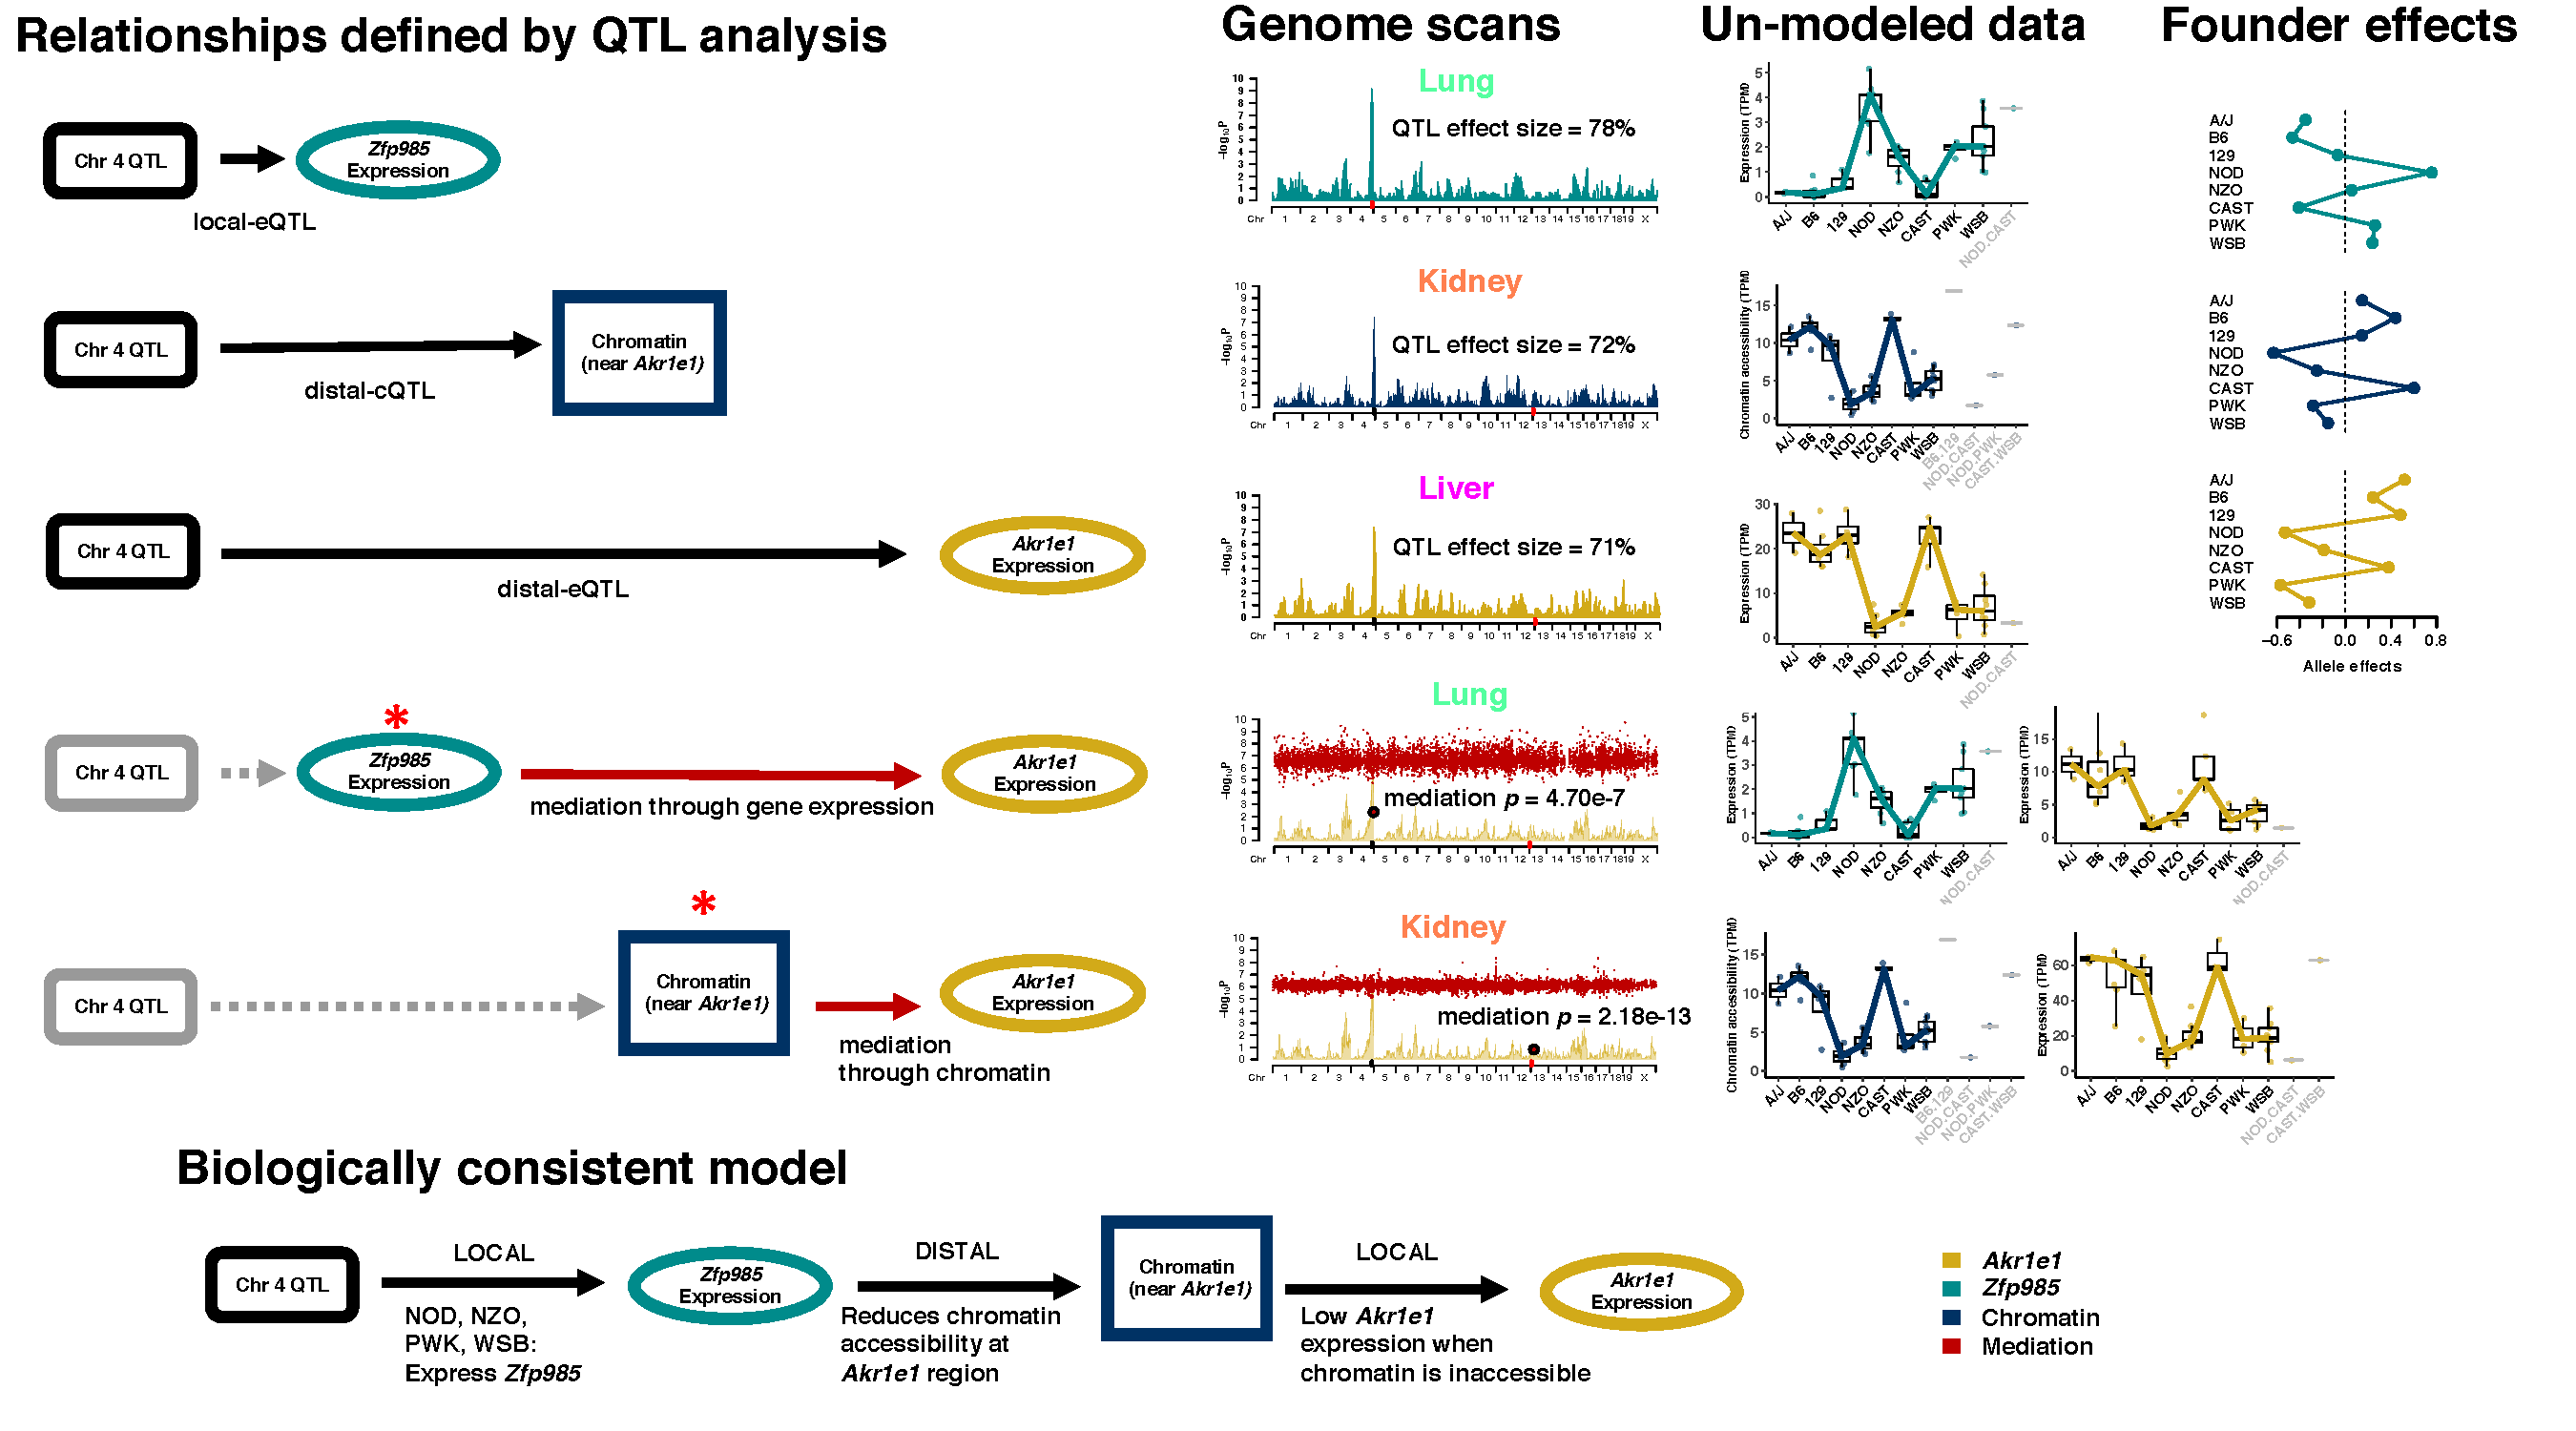
\includegraphics[width=\textwidth, trim={0in 0.1in 0in 0in}, clip]{figs/akr1e1_full_model.pdf}
\caption{\textbf{Complete mediation model for \textit{Akr1e1} distal-eQTL.}  The genetic regulation of \textit{Akr1e1} expression is reconstructed based on relationships observed across the three tissues. Distal-eQTL are detected in all tissues at similar levels of significance. A local-eQTL for \textit{Zfp985} that is proximal to the \textit{Akr1e1} distal-eQTL was observed in lung, and \textit{Zfp985} expression is detected as anti-correlated mediator of the distal-eQTL, consistent with \textit{Zfp985} suppressing \textit{Akr1e1} expression. The chromatin site proximal to the \textit{Akr1e1} TSS has a distal-cQTL detected in kidney. The chromatin accessibility at the site was found to be a significant correlated mediator of \textit{Akr1e1} expression. Combining associations across tissues supports a biological model whereby \textit{Zfp985}, expressed in mice with NOD, NZO, PWK, and WSB alleles, inhibits the proximal chromatin accessibility at the \textit{Akr1e1} TSS. QTL and mediation genome scans are included, along with sequence phenotypes as boxplots categorized according to most likely diplotype, and modeled founder effects fit as BLUPs. The relative magnitudes of the QTL effect sizes (estimated from Eq \ref{eq:effect_size}) and mediation significance are consistent with the proposed model, with \textit{Zfp985} local-eQTL > chromatin distal-eQTL > \textit{Akr1e1} distal-eQTL and chromatin mediation > mediation through \textit{Zfp985} expression.
\label{fig:akr1e1_full_model}}
\end{figure*}

\subsection{Proposed model for the genetic regulation of \textit{Akr1e1} expression}

As detailed above, \textit{Akr1e1} possesses a strong distal-eQTL, observed in all three tissues with significantly correlated founder effects. Additionally, we found that this effect is strongly mediated through Zinc finger protein 985 (\textit{Zfp985}) expression in lung. The \textit{Zfp985} TSS is located on chromosome 4 at 147.6 Mb, while the \textit{Akr1e1} distal-eQTL coordinates are 142.5 Mb, 143.2 Mb, and 148.6 Mb in liver, lung, and kidney, respectively (\textbf{Figure \ref{fig:akr1e1_exmediation}}). \textit{Akr1e1} and \textit{Zfp985} expression are negatively correlated ($r = -0.69$), which is consistent with \textit{Zfp985} inhibiting \textit{Akr1e1} expression. This same distal-eQTL and mediator relationship for \textit{Akr1e1} was observed in pancreatic islet tissue in DO mice \citep{Keller2018}.
The presence of distal genetic regulation for \textit{Akr1e1} was previously described in \cite{HamiltonWilliams2013}. The distal-eQTL we detect are highly proximal to their \textit{Idd9.2} region \citep{HamiltonWilliams2010}, originally defined as spanning 145.5-148.57 Mb of chromosome 4 and subsequently using NOD mice congenic with C57BL/10 (B10) introgressions \cite{HamiltonWilliams2013}. The B10 allele was found to be protective against the development of diabetes, characteristic of NOD mice. \textit{Akr1e1} is involved in glycogen metabolism and the larger \textit{Idd9} region harbors immune-related genes, implicating \textit{Akr1e1} and other genes located in and regulated by \textit{Idd9} as potential diabetes-related genes. 
Consistent with these studies, CC strains with NOD inheritance at the distal-eQTL have low expression of \textit{Akr1e1}. Genetic variation from B10 is not present in the CC, but the closely related B6 founder has high expression of \textit{Akr1e1} like B10. Similar to NOD, NZO, PWK, and WSB alleles result in low \textit{Akr1e1} expression, while A/J, 129, and CAST alleles join B6 as driving high expression (\textbf{Figure \ref{fig:akr1e1_full_model}}). Lowly expressed \textit{Zfp985} is a strong candidate for driving these effects on \textit{Akr1e1}.

Further elucidation of the genetic regulation of \textit{Akr1e1} was observed in kidney tissue, where a strong distal-cQTL is mapped to the \textit{Idd9.2} region for the chromatin site proximal to \textit{Akr1e1}. Based on the close proximities of the chromatin window to \textit{Akr1e1} and the distal-cQTL to the distal-eQTL, we mediated the distal-eQTL effect on the chromatin window, which was highly significant (permP = $\num{2.18e-13}$). The founder effects for the distal-cQTL are correlated with the distal-eQTL effects correlated ($r = 0.92$). The relative magnitudes of the QTL effect sizes and mediation p-values, shown in \textbf{Figure \ref{fig:akr1e1_relationships}}, support a causal model whereby \textit{Zfp985} expression reduces the expression of \textit{Akr1e1} by altering chromatin accessibility in the \textit{Akr1e1} proximal promoter region (\textbf{Figure \ref{fig:akr1e1_full_model}}). 

\subsection{Overview of QTL and mediation analyses}

All QTL and mediation results for all three tissues are depicted as circos plots \citep{Gu2014} in \textbf{Figure \ref{fig:circos_plot}}. Notably, local-QTL and chromatin mediation are not evenly distributed across the genome, but tend to aggregate in pockets. In particular, there is a high concentration of cQTL and chromatin mediation detected along chromosome 17, observed across all three tissues, which happens to correspond to the immune-related major histocompatibility (MHC) region in mouse. However, we note that most of the chromatin-mediated genes in this region are not histocompatibility genes (\textbf{Tables SXX}). The patterns of distal-QTL and gene mediation appear to be tissue-specific, though there are consistent regions observed across the tissues, such as the \textit{Idd9} region \citep{HamiltonWilliams2010} of chromosome 4, which contains multiple zinc finger proteins and regulates genes such as \textit{Akr1e1} and \textit{Ccnyl1}. Previously discussed genes are highlighted for each tissue.

\begin{figure*}[h!]
\renewcommand{\familydefault}{\sfdefault}\normalfont
\centering
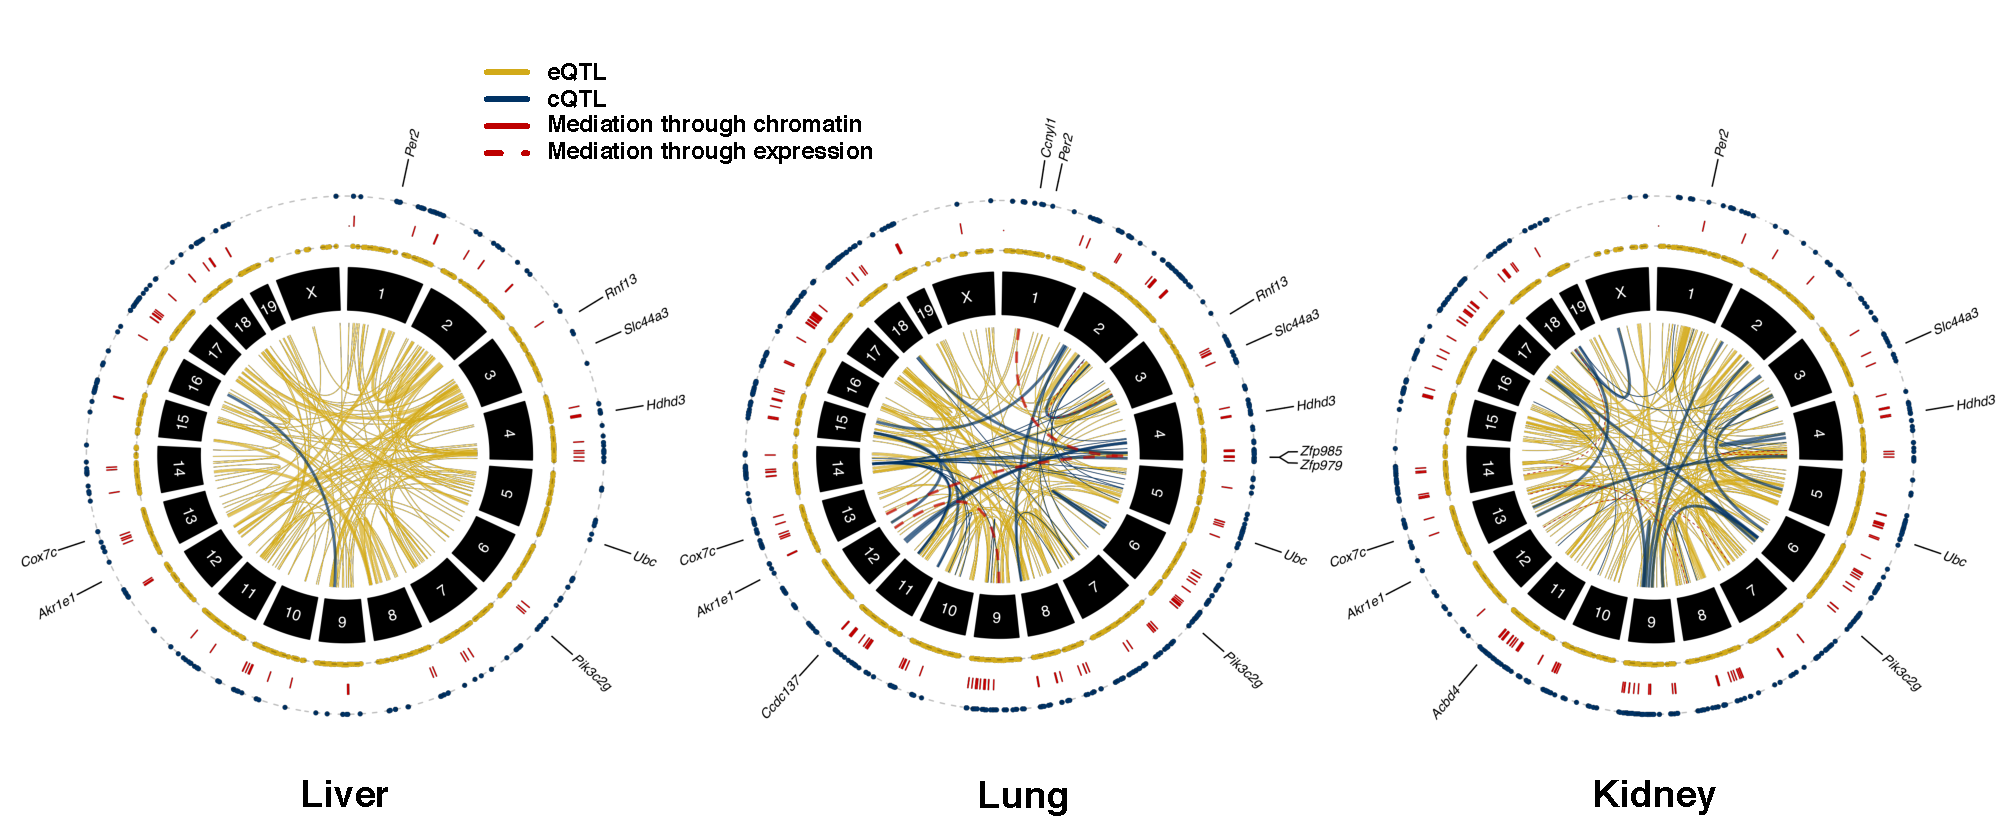
\includegraphics[width=\textwidth, trim={0in 0in 0in 0in}, clip]{figs/circos_over_tissues.pdf}
\caption{\textbf{Summaries of QTL and mediation analyses.} Circos plots of eQTL (yellow), cQTL (blue), and mediation (red) in lung, liver, and kidney. The two outer rings of dots represent local-eQTL and local-cQTL detected by Method 3 at chromosome-wide significance, with red lines between connecting genes and chromatin sites for which chromatin mediation was detected. The inner circle contains connections representing distal-eQTL, distal-cQTL, and gene-gene mediation from Method 1. Thick lines represent QTL and mediators with permutation-based p-value (permP) $< \num{1e-5}$. The detected signals are primarily local, which also tend to be stronger than the observed distal signals. Fewer QTL and mediators are detected in liver tissue. 
%Chromosome 17 has the most concentrated chromatin mediation signal across the three tissues. 
Genes highlighted previously, such as \textit{Akr1e1}, are indicated at their genomic coordinates.
\label{fig:circos_plot}}
\end{figure*}



\section{Discussion}

We perform QTL mapping of gene expression and chromatin accessibility in 47 CC strains. We describe multiple approaches of varying statistical stringency to allow for detection of lower effect local-QTL, important in a study with a restricted sample size. 

Furthermore, we describe statistical approaches for two models of the mediation of the eQTL effect, one through local chromatin accessibility, and the other through an interaction with another gene, measured through its expression, such as a transcription factor, for specifically distal-eQTL. We oriented our mediation through chromatin accessibility to local-eQTL, for which this study is better powered, and find significant support that mediation through chromatin is present (4.2-9.6\% of local-eQTL across the tissues). Certain regions of the genome could not be assessed for chromatin mediation (or cQTL) because ATAC-seq read alignment ambiguity, further restricting our ability to assess mediation. Despite these constraints, the results are still consistent with the assertion that chromatin plays a role in the regulation of gene expression \citep{Klemm2019}. In terms of gene expression mediators of distal-eQTL, though we are likely poorly powered to detect them, we do find a number of strong candidates, specifically of zinc finger protein genes acting as mediators. 

\subsection{Multiple procedures for QTL detection}

The use of multiple criteria for detection allowed us to assess varying degrees of statistical support for the associations, and in particular, leverage the prior belief in local associations in order to detect higher numbers of QTL for a relatively small sample of 47 mice. The multi-stage procedure allows for genome-wide detection of QTL that incorporates both FWER and FDR adjustments. Both the chromosome-wide FDR and single step analyses strongly increase power to detect local-QTL, but lose the ability to adequately accommodate distal-QTL.

% \subsection{Distal-QTL on local chromosome}

% We find that we are powered to detect distal-QTL predominately located on the local chromosome, as seen in \textbf{Figure \ref{fig:grid_plot}}. Many FWER-significant (permP < 0.05) distal-QTL on non-local chromosomes are filtered by the FDR procedure, such as the distal-eQTL for \textit{Ccnyl1}, shown in \textbf{Figure \ref{fig:exmediation}}. The mediation of this distal-eQTL through zinc finger proteins strongly suggests that it is a real distal-eQTL. It is possible that distal-QTL on non-local chromosomes tend to be of lower effect than distal-QTL located on the local chromosome, though far from the gene or chromatin site, and these data are not sufficiently powered to detect non-local chromosome distal-QTL. 

\subsection{QTL effect size}

Estimation of the variance explained by the QTL, referred to as the effect size, can provide a point summary for haplotype-based QTL mapping, analogous to the effect of the minor allele, which is commonly used in SNP association. Fitting the QTL effect as a random term, and thus inducing conservative shrinkage on the effect size, can highlight QTL detections that are likely based on unstable fixed effects from influential data points. Notably, a number of the genome-wide significant distal-eQTL have very low effect size estimates (\textbf{Figure \ref{fig:qtl_effect_sizes_strict} [top]}) in comparison to the effects sizes seen in local-eQTL, even when detected with more lenient procedures, as in \textbf{Figure \ref{fig:qtl_effect_sizes_permissive} [top]}. A mapping procedure that fits the QTL effect as a random effect, as in \cite{Wei2016}, would not detect these QTL. However, a random effects procedure is more computationally intensive, which is particularly prohibitive in the context of genome-wide traits, thus justifying a follow-up approach in which effect sizes are evaluated for the detected QTL.

\subsection{QTL mapping tissues jointly}

\subsection{Mediation}

Our mediation approach uses a similar approach to that previously done with DO mice \citep{Chick2016,Keller2018}, though with some modification and to our knowledge, it has never been used in the CC. Notably we use a permutation procedure in which the mediator variable is permuted to determine empirical thresholds of significance. We also filter out mediators based on QTL effect sizes that are consistent with the proposed models of mediation. Mediation within the field of system genetics is a growing area of interest, and the methods proposed here support that development.

\section{Acknowledgments}
Author contributions: GRK, BQ, and TSF wrote the manuscript. GRK and WV developed the statistical methods for QTL analysis, and GRK wrote the software to perform the respective analyses. BQ processed the sequence data and performed the differential expression and accessible analyses. GRK and BQ performed all QTL and mediation analyses. The authors declare no conflicts of interest.

\bibliography{eQTL_mediation.bib}

\clearpage

\section{Appendix A: False positive control}

\subsection{Family-wide error rate}

The family-wide error rate (FWER) is the probability of detecting a single false positive across all genome-wide tests. Controlling FWER instead of the single test type I error rate ($\alpha$) is necessary because FWER increases with the number independent tests, reaching 1 for $\alpha = 0.05$ in the context of genome-wide tests. Controlling FWER is more conservative than controlling the false discovery rate (FDR) for multiple testing correction, and appropriate for genome scans of a single trait because there are not expected to be an excess number of QTL per outcome. 

Based on simulations of the breeding design \citep{Valdar2006c}, the CC panel was expected to be balanced in terms of founder haplotype contributions. This balance was realized to large extent \citep{Srivastava2017}, though the PWK and CAST founders have reduced contributions in comparison to the other founders. \cite{KeeleSPARCC} performed simulations from the realized CC strain genomes to examine QTL mapping power, and found low levels of population structure in the CC genomes, violating the exchangeability assumption made by the permutation procedure, which characterizes a null distribution for the test statistic\citep{Doerge1996}. Nevertheless, we use a permutation approach, given that we expect the presence of strong effect QTL for the molecular traits that are detectable in the presence of subtle population structure.

Specifically, 1000 permutations of the sample identities were taken, and then genome scans performed on each permutation of each trait. For each trait, the minimum p-value from each permutation genome scan is recorded, transformed to the -$\log_{10}$ scale (logP), and then used fit a null extreme value distribution (EVD) \citep{Dudbridge2004,Valdar2006c}. Genome-wide permutation-based p-values (permP) are obtained by calculating the probability of a more extreme logP than the observed from the cumulative distribution function of the EVD.

\subsection{False discovery rate}

Analyzing a large numbers of traits, as is the case with gene expression and chromatin accessibility, also contributes significantly to a multiple testing burden. Not only is an association for a trait being tested at positions across the genome, but the whole process is repeated per trait. The expected number of significant tests is also different globally across all the traits, with many traits expected to have QTL in comparison to there being few QTL for a single trait. 

An FDR procedure can address this multiple testing dynamic, accounting for the additional testing due to genome-wide traits while being more lenient than strict FWER control across traits. As in \cite{Chick2016}, an FDR procedure \citep{Benjamini1995,Storey2003} is applied to the per-trait FWER-adjusted permP, producing q-values. QTL are detected if q-value $\le \alpha_{\text{FDR}}$, where $\alpha_{\text{FDR}}$ is the specified false discovery rate. QTL were called using both $\alpha_{\text{FDR}} = 0.1$ and $\alpha_{\text{FDR}} = 0.2$.

\section{Appendix B: Mapping procedures}

\subsection{Method 1: Multi-stage conditional regression with genome-wide FWER and FDR}

The combined per-trait FWER control and across-trait FDR control restrict the mapping procedure’s ability to detect multiple QTL per outcome in a statistically valid manner because the EVD used for FWER adjustment is fit from the maximum statistical score per trait. To include additional strong statistical scores is potentially biasing, as would be the case when there are multiple associations above the FWER threshold, increasing the enrichment in small p-values. This inflations in small p-values is precisely the pattern of association the FDR procedure detects. To avoid this problem, a multi-stage conditional fitting approach is used \citep{Jansen2017}. The procedure is described in the following steps:
\begin{enumerate}
	\item For a given trait, conduct genome scan according to the model described in Eq \ref{eq:alternative_model}.
    \item Perform genome scans for the permuted trait to characterize an EVD. Calculate FWER-adjusted permP from the observed maximum logP of the genome scan of the trait. The permP is stored to be used as input to an FDR method.
    \item Specify a genome-wide $\alpha_{\text{step}}$ for determining whether subsequent conditional scans should be conducted for the trait. We set $\alpha_{\text{step}} = 0.1$. If the $\text{permP} > \alpha_{\text{step}}$, no further conditional scans are conducted.
    \item If $\text{permP} \le \alpha_{\text{step}}$, steps 1-3 are repeated for additional conditional scans of the outcome. For $j > 1$, $j^{\text{th}}$ conditional scan use the same form of alternative and null model as described in Eq \ref{eq:alternative_model}, except with the inclusion of locus effects from the peak associations from previous stages. Generally, the alternative model for conditional stage scan $J$ follows as:
\begin{equation}
y_{i} = \mu + \text{QTL}_{i} + \sum_{j=1}^{J-1}\text{locus}_{i}^{j} + \text{batch}_{i} + \varepsilon_{i},
\label{eq:conditional_model}
\end{equation}
with $\text{locus}_{i}^{j}$ representing the locus effect of the peak association from the $j^{\text{th}}$ stage scan of the outcome for individual $i$, and is also included in the null model of conditional scans. Now steps 2-4 are repeated.
\end{enumerate}

A multi-stage conditional scan approach could have issues with over-fitting 47 data points per trait, given that each $\text{QTL}$ and $\text{locus}$ effect represents the estimation of seven fixed effects. However, the permutations were found to appropriately compensate for this potential in the recalculation of the EVD based on permutations of the conditional scans in step 2. \textbf{Figure \ref{fig:conditional_scans}} provides a clear example in which the gene \textit{Gpn3} has a local-eQTL detected after a strong distal-eQTL is conditioned for within the model in lung tissue. This multi-stage conditional procedure is referred to as Method 1.

\subsection{Method 2: Single-stage regression with chromosome-wide FWER and FDR control}

Given that the data represent 47 individual mice, there may be poor power to detect genome-wide significant QTL. Because of the strong biological prior evidence for local-QTL, significant genetic associations that meet chromosome-wide significance for the local chromosome of the trait were also detected and recorded. This was accomplished by fitting a chromosome-wide EVD, and thus producing chromosome-wide FWER-adjusted permP for each trait. Chromosome-wide results were restricted to the first stage of the multi-stage procedure, thus referred to as a single-stage analysis, and allowing only a single chromosome-wide permP per trait. The same FDR then used as in Method 1, resulting in chromosome-wide q-values. This more lenient single-stage procedure is referred to as Method 2.

\subsection{Method 3: Single-stage regression with genome-wide and chromosome-wide FWER control for local-QTL}

A final local-QTL exclusive single step analysis is used. Instead of calculating genome-wide and chromosome-wide permP from the overall maximum logP, FWER-controlled permP are adjusted from the maximum logP within the proximal window of the trait from the first stage scans from Method 1. An FDR procedure is not used, in part because the permP are likely to be poorly distributed with respect to the expectations of FDR. A local-QTL is detected when $\text{permP} < 0.05$. This procedure, now referred to as Method 3, is less conservative for local-QTL because there is no FDR control, instead leveraging the strong biological precedent for proximal genetic regulation. It also does not leniently detect intra-chromosomal distal-QTL, as with Method 2.

\section{Appendix C: Mediation analysis}

\subsection{Mediation models}

\subsubsection{Mediation of local-eQTL through chromatin state.}
Mediation through chromatin accessibility was evaluated for all local-eQTL detected through the lenient Method 3, leveraging prior knowledge of the predominance of local genetic regulation and the effects of proximal chromatin state. Candidate mediators are detected at genome and chromosome-wide significance through 1,000 permutations to define EVD for FWER adjustment.

\subsubsection{Mediation of distal-eQTL through proximal gene expression.}
Mediation of the effect of genome-wide significant distal-eQTL through proximal gene expression was evaluated. Genome-wide significance is required for distal-eQTL because there is not additional strong biological information to support increased leniency as is the case with proximal signal. As with mediation through chromatin state, 1,000 permutations are used to define mediation significance thresholds at the genome-wide level. 

Mediation of cQTL through other chromatin sites and gene expression were also evaluated, but did not result in the detection of any candidate mediators.

\subsection{Mediation significance thresholds}

Empirical significance thresholds for the mediation scans can be defined through permutations, similarly to as is done with the QTL scans. Instead of permuting the trait outcome, the pairing of trait to QTL is maintained, and the mediator is permuted. EVD are then fit for potential mediators from the minimum logP from permutation scans, instead of the maximum logP in QTL scans. FWER-adjusted mediation permP are extracted from the EVD, which can be calculated in terms of genome-wide and chromosome-wide significance. An FDR adjustment is not used with mediation because it is only evaluated for detected QTL, which could potentially violate the uniform null distribution expectations of FDR.

\subsection{Formal mediation criterion}

Detection of mediation has some caveats and pitfalls compared to the statistical analyses used for QTL mapping, in part due to the fact that the relationships \ref{rel:eQTL} and \ref{rel:cQTL} could be complex, whereas the directionality of the relationships for QTL is fixed because the genetic state at the QTL cannot change due because of the trait. This does not hold for the mediation model, where Y could in fact causally influence M (Y $\rightarrow$ M). \cite{Didelez2007} note that false mediation signals can be detected when the association between the M and Y are particularly strong, whereby M acts as a surrogate for X. Based on concerns over fitting relatively complex models to data comprising 47 observations, we use stringent requirements for declaring evidence for mediation:
\begin{enumerate}
	\item Detection of a significant eQTL (relationship \ref{rel:eQTL}).
    \begin{enumerate}
    	\item Mediation through chromatin: chromosome-wide permP < 0.05 from Method 3
        \item Mediation through expression: genome-wide q-value < 0.1 from Method 1
    \end{enumerate}
    \item Detection of significant mediator within a 20 Mb window centered around the eQTL from previous step.
    \item Detection of a significant QTL for the mediator from previous step.
    \begin{enumerate}
    	\item Mediation through chromatin: chromosome-wide permP < 0.05 from Method 3 and within 10 Mb upstream or downstream of gene TSS
        \item Mediation through expression: genome-wide q-value < 0.1 from Method 1 and within 10 Mb upstream or downstream of the eQTL position
    \end{enumerate}
    \item It is not possible to distinguish M $\rightarrow$ Y from M $\leftarrow$ Y given these data. If M is an intermediary of X on Y, the expectation is that the effect of X $\rightarrow$ M is greater than X $\rightarrow$ Y. We check that the effect size of the QTL for step 1 (X $\rightarrow$ Y) is less than the effect size of the QTL from step 3 (X $\rightarrow$ M), based on Eq \ref{eq:effect_size}. Failure of this step does not disprove the proposed mediation model, but it could suggest that the relationship between M and Y is more complicated than the simple models tested here, or that greater noise is incurred in the measurement of M than Y.
\end{enumerate}

\clearpage

\section{Data and Supplement details}

\thispagestyle{empty}
\clearpage

\section{Supplemental Tables and Figures}
\setcounter{table}{0}
\setcounter{figure}{0}
\renewcommand{\thetable}{S\arabic{table}}
\renewcommand{\thefigure}{S\arabic{figure}}
\setcounter{page}{1}

\begin{table*}[h]
\renewcommand{\familydefault}{\sfdefault}\normalfont
\begin{tableminipage}{\textwidth}
\captionsetup{width=\textwidth}
\centering
\caption{\bf Number of differentially expressed genes and accessible chromatin regions detected between liver, lung, and kidney tissues
\label{tab:diff_gene}}
\end{tableminipage}
\begin{tableminipage}{\textwidth}
\begin{tabularx}{\textwidth}{cll|XXX}
\hline 
& & & & \center{Tissue comparison} & \\
& & & Liver vs Lung & Liver vs Kidney & Lung vs Kidney \\
\hline
%%%%%%%%%%%%%%%%
\parbox[t]{5mm}{\multirow{6}{*}{\rotatebox[origin=c]{90}{q-value < 0.1}}} & 
Genes & Up-regulated & 2,473 (20.8\footnote{Percentage of all tested genes.\label{fn:total_perc_gene}}) & 2,123 (17.9\footref{fn:total_perc_gene}) & 2,246 (18.9\footref{fn:total_perc_gene}) \\
& & Down-regulated & 3,236 (27.2\footref{fn:total_perc_gene}) & 1,441 (12.1\footref{fn:total_perc_gene}) & 2,527 (21.3\footref{fn:total_perc_gene}) \\
& & Total & 5,709 (48.0\footref{fn:total_perc_gene}) & 3,564 (30.0\footref{fn:total_perc_gene}) & 4,773 (40.2\footref{fn:total_perc_gene}) \\
\cline{2-6}
& Chromatin Regions & Increased accessibility & 20,194 (19.6\footnote{Percentage of all tested chromatin regions prior to merging adjacent genomic windows.\label{fn:total_perc_chrom}}) & 15,252 (12.9\footref{fn:total_perc_chrom}) & 19,202 (17.4\footref{fn:total_perc_chrom}) \\
& & Decreased accessibility & 20,603 (19.7\footref{fn:total_perc_chrom}) & 12,796 (11.4\footref{fn:total_perc_chrom}) & 12,967 (11.2\footref{fn:total_perc_chrom}) \\
& & Total & 40,797 (39.3\footref{fn:total_perc_chrom}) & 28,048 (24.3\footref{fn:total_perc_chrom}) & 32,169 (28.6\footref{fn:total_perc_chrom}) \\
\hline
\end{tabularx}
\end{tableminipage}
\end{table*}

\begin{table*}[h]
\renewcommand{\familydefault}{\sfdefault}\normalfont
\begin{tableminipage}{\textwidth}
\captionsetup{width=\textwidth}
\centering
\caption{\bf Number of genes with eQTL detected in liver, lung, and kidney tissues
\label{tab:eqtl_mapping}}
\end{tableminipage}
\begin{tableminipage}{\textwidth}
\begin{tabularx}{\textwidth}{ll|XXX}
\hline 
& & & \center{Tissue (\%)} & \\
Procedure & eQTL type & Liver & Lung & Kidney \\
\hline
%%%%%%%%%%%%%%%%
Method 1\footnote{Multi-stage conditional regression analysis with genome-wide FDR < 0.1. \label{fn:method_one}} & All & 520 (6.2\footnote{Percentage of all tested genes.\label{fn:total_perc}}) & 478 (4.2\footref{fn:total_perc}) & 739 (7.3\footref{fn:total_perc}) \\
& Local\footnote{10 Mb upstream or downstream of gene TSS. \label{fn:local_eqtl}} & 400 (76.9\footnote{Percentage of genes with genome-wide eQTL.\label{fn:gw_eqtl_perc}}) & 369 (77.2\footref{fn:gw_eqtl_perc}) & 601 (81.3\footref{fn:gw_eqtl_perc}) \\
& Distal\footnote{More than 10 Mb upstream or downstream of gene TSS or on another chromosome. \label{fn:distal_eqtl}} & 132 (25.4\footref{fn:gw_eqtl_perc}) & 112 (23.4\footref{fn:gw_eqtl_perc}) & 148 (20.0\footref{fn:gw_eqtl_perc}) \\
\hline
% %%%%%%%%%%%%%%%%
Method 2\footnote{Single-step regression analysis with chromosome-wide FDR < 0.1. \label{fn:method_two}} & All & 2,587 (30.8\footref{fn:total_perc}) & 2,069 (18.2\footref{fn:total_perc}) & 3,191 (31.6\footref{fn:total_perc}) \\
& Local\footref{fn:local_eqtl} & 1,749 (67.6\footnote{Percentage of genes with chromosome-wide eQTL.\label{fn:cw_eqtl_perc}}) & 1,498 (72.4\footref{fn:cw_eqtl_perc}) & 2,214 (69.4\footref{fn:cw_eqtl_perc}) \\
& Distal\footref{fn:distal_eqtl} & 838 (32.4\footref{fn:cw_eqtl_perc}) & 571 (27.6\footref{fn:cw_eqtl_perc}) & 977 (30.6\footref{fn:cw_eqtl_perc}) \\
\hline
% %%%%%%%%%%%%%%%%
Method 3\footnote{Single-step regression analysis restricted to local signals and with FWER p-value < 0.05. \label{fn:method_three}} & Local\footref{fn:local_eqtl} genome-wide & 702 (8.4\footref{fn:total_perc}) & 713 (6.3\footref{fn:total_perc}) & 955 (9.5\footref{fn:total_perc}) \\
& Local\footref{fn:local_eqtl} chromosome-wide & 1,661 (19.8\footref{fn:total_perc}) & 1,880 (16.6\footref{fn:total_perc}) & 2,102 (20.8\footref{fn:total_perc}) \\
% & chromatin mediator\footnote{Must be within 10 Mb upstream or downstream of an local-eQTL that is at least chromosome-wide significant. Additionally, chromatin mediator must possess a local c-QTL that is at least chromosome-wide significant.} & genome-wide & 38 (2.2\footnote{Percentage of genes with a chromatin mediator that have at least a chromosome-wide significant local-eQTL from local analysis.\label{fn:mediator_perc}}) & 13 (0.9\footref{fn:mediator_perc}) & 19 (1.0\footref{fn:mediator_perc}) \\
% & chromosome-wide & 99 (5.9\footref{fn:mediator_perc}) & 30 (2.0\footref{fn:mediator_perc}) & 49 (2.6\footref{fn:mediator_perc}) \\
\hline
\end{tabularx}
\end{tableminipage}
\end{table*}

\begin{table*}[h]
\renewcommand{\familydefault}{\sfdefault}\normalfont
\begin{tableminipage}{\textwidth}
\captionsetup{width=\textwidth}
\centering
\caption{\bf Number of genes with eQTL detected in liver, lung, and kidney tissues at FDR < 0.2
\label{tab:eqtl_mapping_lenient}}
\end{tableminipage}
\begin{tableminipage}{\textwidth}
\begin{tabularx}{\textwidth}{ll|XXX}
\hline 
& & & \center{Tissue (\%)} & \\
Procedure & eQTL type & Liver & Lung & Kidney \\
\hline
%%%%%%%%%%%%%%%%
Method 1\footnote{Multi-stage conditional regression analysis with genome-wide FDR < 0.2.} & All & 881 (10.5\footref{fn:total_perc}) & 811 (7.1\footref{fn:total_perc}) & 1,189 (11.8\footref{fn:total_perc}) \\
& Local\footnote{10 Mb upstream or downstream of gene TSS. \label{fn:local_eqtl}} & 568 (64.5\footref{fn:gw_eqtl_perc}) & 522 (64.4\footref{fn:gw_eqtl_perc}) & 809 (68.0\footref{fn:gw_eqtl_perc}) \\
& Distal\footnote{More than 10 Mb upstream or downstream of gene TSS or on another chromosome. \label{fn:distal_eqtl}} & 339 (38.5\footref{fn:gw_eqtl_perc}) & 301 (37.1\footref{fn:gw_eqtl_perc}) & 411 (34.6\footref{fn:gw_eqtl_perc}) \\
\hline
% %%%%%%%%%%%%%%%%
Method 2\footnote{Single-step regression analysis with chromosome-wide FDR < 0.2.} & All & 4,699 (55.9\footref{fn:total_perc}) & 3,675 (32.4\footref{fn:total_perc}) & 5,469 (54.2\footref{fn:total_perc}) \\
& Local\footref{fn:local_eqtl} & 2,519 (53.6\footnote{Percentage of genes with chromosome-wide eQTL.\label{fn:cw_eqtl_perc}}) & 2,213 (60.2\footref{fn:cw_eqtl_perc}) & 3,099 (56.7\footref{fn:cw_eqtl_perc}) \\
& Distal\footref{fn:distal_eqtl} & 2,180 (46.4\footref{fn:cw_eqtl_perc}) & 1,462 (39.8\footref{fn:cw_eqtl_perc}) & 2,370 (43.3\footref{fn:cw_eqtl_perc}) \\
\hline
\end{tabularx}
\end{tableminipage}
\end{table*}

\begin{table*}[h]
\renewcommand{\familydefault}{\sfdefault}\normalfont
\begin{tableminipage}{\textwidth}
\captionsetup{width=\textwidth}
\centering
\caption{\bf Number of chromatin accessibility sites with cQTL detected in liver, lung, and kidney tissues
\label{tab:cqtl_mapping}}
\end{tableminipage}
\begin{tableminipage}{\textwidth}
\begin{tabularx}{\textwidth}{ll|XXX}
\hline 
& & & \center{Tissue (\%)} & \\
Procedure & cQTL type & Liver & Lung & Kidney \\
\hline
%%%%%%%%%%%%%%%%
Method 1\footnote{Multi-stage conditional regression analysis with genome-wide FDR < 0.1.} & All & 17 (0.1\footnote{Percentage of all tested chromatin site.\label{fn:total_perc}}) & 114 (0.5\footref{fn:total_perc}) & 59 (0.3\footref{fn:total_perc}) \\
& Local\footnote{10 Mb upstream or downstream of the midpoint of the chromatin accessibility site. \label{fn:local_cqtl}} & 16 (94.1\footnote{Percentage of chromatin accessibility sites with genome-wide cQTL.\label{fn:gw_cqtl_perc}}) & 78 (68.4\footref{fn:gw_cqtl_perc}) & 39 (66.1\footref{fn:gw_cqtl_perc}) \\
& Distal\footnote{More than 10 Mb upstream or downstream of the midpoint of the chromatin accessibility site or on another chromosome. \label{fn:distal_cqtl}} & 1 (5.9\footref{fn:gw_cqtl_perc}) & 36 (31.6\footref{fn:gw_cqtl_perc}) & 20 (33.9\footref{fn:gw_cqtl_perc}) \\
\hline
% %%%%%%%%%%%%%%%%
Method 2\footnote{Single-step regression analysis with chromosome-wide FDR < 0.1.} & All & 39 (0.3\footref{fn:total_perc}) & 226 (0.9\footref{fn:total_perc}) & 130 (0.7\footref{fn:total_perc}) \\
& Local\footref{fn:local_cqtl} & 35 (89.7\footnote{Percentage of chromatin accessibility sites with chromosome-wide cQTL.\label{fn:cw_cqtl_perc}}) & 186 (82.3\footref{fn:cw_cqtl_perc}) & 98 (75.4\footref{fn:cw_cqtl_perc}) \\
& Distal\footref{fn:distal_cqtl} & 4 (10.3\footref{fn:cw_cqtl_perc}) & 40 (17.7\footref{fn:cw_cqtl_perc}) & 32 (24.6\footref{fn:cw_cqtl_perc}) \\
\hline
% %%%%%%%%%%%%%%%%
Method 3\footnote{Single-step regression analysis restricted to local signals and with FWER p-value < 0.05.} & Local\footref{fn:local_cqtl} genome-wide & 70 (0.6\footref{fn:total_perc}) & 244 (1.0\footref{fn:total_perc}) & 149 (0.8\footref{fn:total_perc}) \\
& Local\footref{fn:local_cqtl} chromosome-wide & 299 (2.6\footref{fn:total_perc}) & 876 (3.6\footref{fn:total_perc}) & 616 (3.4\footref{fn:total_perc}) \\
% & chromatin mediator\footnote{Must be within 10 Mb upstream or downstream of an local-eQTL that is at least chromosome-wide significant. Additionally, chromatin mediator must possess a local c-QTL that is at least chromosome-wide significant.} & genome-wide & 38 (2.2\footnote{Percentage of genes with a chromatin mediator that have at least a chromosome-wide significant local-eQTL from local analysis.\label{fn:mediator_perc}}) & 13 (0.9\footref{fn:mediator_perc}) & 19 (1.0\footref{fn:mediator_perc}) \\
% & chromosome-wide & 99 (5.9\footref{fn:mediator_perc}) & 30 (2.0\footref{fn:mediator_perc}) & 49 (2.6\footref{fn:mediator_perc}) \\
\hline
\end{tabularx}
\end{tableminipage}
\end{table*}

\begin{table*}[h]
\renewcommand{\familydefault}{\sfdefault}\normalfont
\begin{tableminipage}{\textwidth}
\captionsetup{width=\textwidth}
\centering
\caption{\bf Number of chromatin accessibility sites with cQTL detected in liver, lung, and kidney tissues at FDR < 0.2
\label{tab:cqtl_mapping_lenient}}
\end{tableminipage}
\begin{tableminipage}{\textwidth}
\begin{tabularx}{\textwidth}{ll|XXX}
\hline 
& & & \center{Tissue (\%)} & \\
Procedure & cQTL type & Liver & Lung & Kidney \\
\hline
%%%%%%%%%%%%%%%%
Method 1\footnote{Multi-stage conditional regression analysis with genome-wide FDR < 0.1.} & All & 20 (0.2\footref{fn:total_perc}) & 220 (0.9\footref{fn:total_perc}) & 113 (0.6\footref{fn:total_perc}) \\
& Local\footnote{10 Mb upstream or downstream of the midpoint of the chromatin accessibility site. \label{fn:local_cqtl}} & 18 (90.0\footref{fn:gw_cqtl_perc}) & 116 (52.7\footref{fn:gw_cqtl_perc}) & 55 (48.7\footref{fn:gw_cqtl_perc}) \\
& Distal\footnote{More than 10 Mb upstream or downstream of the midpoint of the chromatin accessibility site. \label{fn:distal_cqtl}} & 2 (10.0\footref{fn:gw_cqtl_perc}) & 105 (47.7\footref{fn:gw_cqtl_perc}) & 58 (51.3\footref{fn:gw_cqtl_perc}) \\
\hline
% %%%%%%%%%%%%%%%%
Method 2\footnote{Single-step regression analysis with chromosome-wide FDR < 0.1.} & All & 62 (0.5\footref{fn:total_perc}) & 309 (1.3\footref{fn:total_perc}) & 249 (1.4\footref{fn:total_perc}) \\
& Local\footref{fn:local_cqtl} & 50 (80.6\footref{fn:cw_cqtl_perc}) & 238 (77.0\footref{fn:cw_cqtl_perc}) & 149 (59.8\footref{fn:cw_cqtl_perc}) \\
& Distal\footref{fn:distal_cqtl} & 12 (19.4\footref{fn:cw_cqtl_perc}) & 71 (23.0\footref{fn:cw_cqtl_perc}) & 100 (40.2\footref{fn:cw_cqtl_perc}) \\
\hline
\end{tabularx}
\end{tableminipage}
\end{table*}

\begin{table*}[h]
\renewcommand{\familydefault}{\sfdefault}\normalfont
\begin{tableminipage}{\textwidth}
\captionsetup{width=\textwidth}
\centering
\caption{\bf Number of genes with chromatin mediation of local-eQTL in liver, lung, and kidney tissues
\label{tab:mediation}}
\end{tableminipage}
\begin{tableminipage}{\textwidth}
\begin{tabularx}{\textwidth}{ll|XXX}
\hline 
& & & \center{Tissue (\%)} & \\
Procedure & Significance & Liver & Lung & Kidney \\
\hline
%%%%%%%%%%%%%%%%
Method 3\footnote{10 Mb upstream or downstream of the gene TSS with local-eQTL that meets chromosome-wide significance through Method 3. Additionally, chromatin mediator must possess a local-cQTL that meets chromosome-wide significance through Method 3.} & genome-wide & 13 (0.8\footnote{Percentage of genes with a chromatin mediator that meet chromosome-wide significance for a local-eQTL through Method 3.\label{fn:mediator_perc}}) & 42 (2.2\footref{fn:mediator_perc}) & 21 (1.0\footref{fn:mediator_perc}) \\
& chromosome-wide & 35 (2.1\footref{fn:mediator_perc}) & 106 (5.6\footref{fn:mediator_perc}) & 66 (3.1\footref{fn:mediator_perc}) \\
\hline
\end{tabularx}
\end{tableminipage}
\end{table*}

\begin{table*}[h]
\renewcommand{\familydefault}{\sfdefault}\normalfont
\begin{tableminipage}{\textwidth}
\captionsetup{width=\textwidth}
\centering
\caption{\bf Genes with distal-eQTL with gene mediators detected in lung and kidney tissues
\label{tab:exmediation}}
\end{tableminipage}
\begin{tableminipage}{\textwidth}
\begin{tabularx}{\textwidth}{lll|XXX}
\hline 
Tissue & Gene & Chr & Mediator gene & Chr & permP \\
\hline
%%%%%%%%%%%%%%%%
Lung & \textit{Akr1e1} & 13 & \textit{Zfp985} & 4 & 4.70e-07 \\
& \textit{Ccnyl1} & 1 & \textit{Zfp979} & 4 & 1.71e-10 \\
& & & \textit{Zfp985} & 4 & 1.23e-05 \\ 
& \textit{Man2c1} & 9 & \textit{Vash1} & 12 & 1.77e-06 \\
& \textit{Rbm46} & 3 & \textit{Gatm} & 2 & 1.06e-02 \\
\hline
Kidney & \textit{C330018D20Rik} & 13 & \textit{Depdc1b} & 18 & 9.97e-04 \\
& \textit{Fbln5} & 12 & \textit{Crym} & 7 & 3.67e-02 \\
& \textit{Gcdh} & 8 & \textit{Dmgdh} & 13 & 8.96e-04 \\
& \textit{Oscp1} & 4 & \textit{Slc25a34} & 4 & 3.27e-03 \\
\hline
\end{tabularx}
\end{tableminipage}
\end{table*}

\clearpage

\begin{figure*}[hp]
\renewcommand{\familydefault}{\sfdefault}\normalfont
\centering
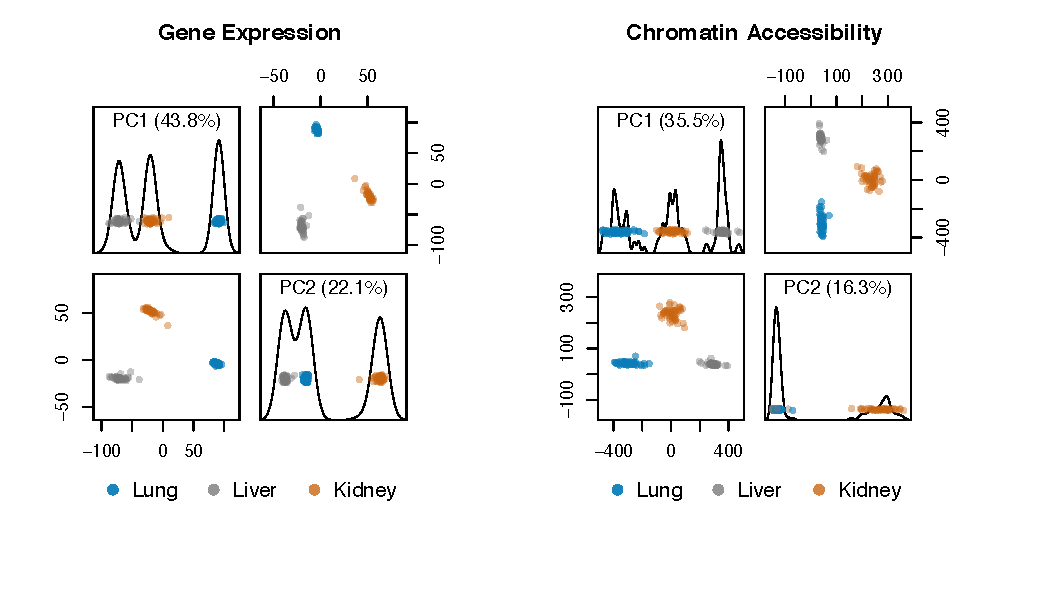
\includegraphics[width=0.8\textwidth, trim={0.25in 0.5in 0.5in 0in}, clip]{figs/pca_plot.pdf}
\caption{\textbf{Principle components analysis identifies tissue type as key source of variation for gene expression and chromatin accessibility.} Molecular traits for lung (blue), liver (gray), and kidney (orange) tissue samples were derived from RNA-seq and ATAC-seq data. Principal components (PC) 1 and 2 capture a majority of the variation and show a greater amount of between tissue variability than within tissue variability. \label{fig:pca_plots}}
\end{figure*}

\begin{figure*}[hp]
\renewcommand{\familydefault}{\sfdefault}\normalfont
\centering
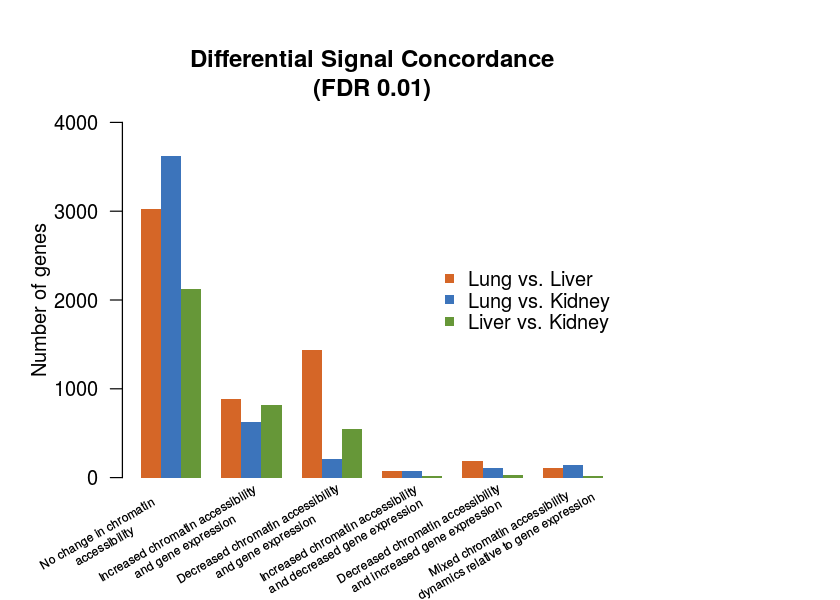
\includegraphics[width=0.8\textwidth, trim={0in 0in 0in 0in}, clip]{figs/diff_concordance.png}
\caption{\textbf{Concordance between differentially expressed (DE) genes and differentially accessible regions (DAR) in between-tissue comparisons.} Genes were categorized by the direction of the difference in expression and chromatin accessibility in their promoter regions.\label{fig:diff_concordance}}
\end{figure*}

\begin{figure*}[hp]
\renewcommand{\familydefault}{\sfdefault}\normalfont
\centering
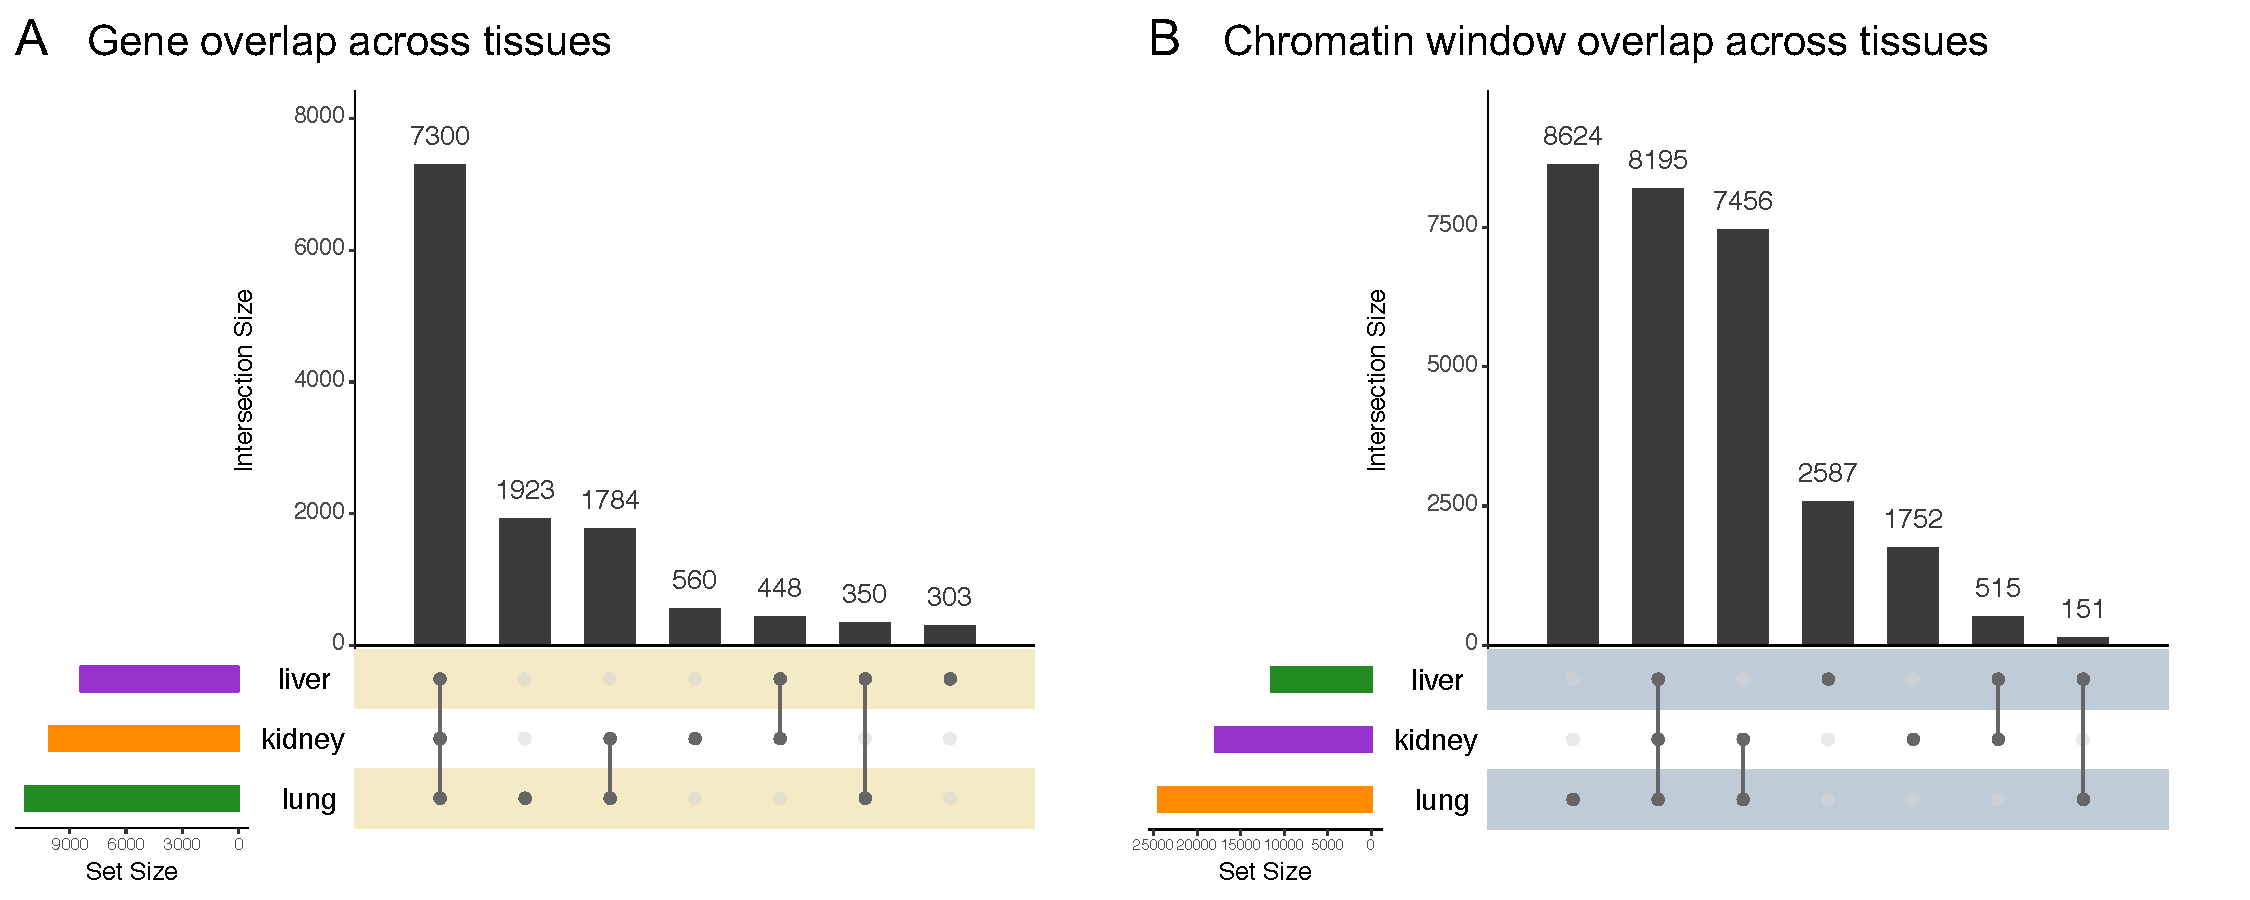
\includegraphics[width=\textwidth, trim={0in 0in 0in 0in}, clip]{figs/upset_genes_chromatin.pdf}
\caption{\textbf{Overlap across tissues of genes and chromatin windows used for QTL analysis.} Sequence traits were filtered to remove outcomes more likely to cause in spurious QTL signal. Genes with TPM $\le 1$ and chromatin windows with TMP $\le 5$ for $\ge$ 50\% of samples were removed from analysis. After this filtering process, lung had the greatest number of traits analyzed, for both genes and chromatin windows, followed by kidney and then liver. 
\label{fig:upset_genes_chromatin}}
\end{figure*}

\begin{figure*}[hp]
\renewcommand{\familydefault}{\sfdefault}\normalfont
\centering
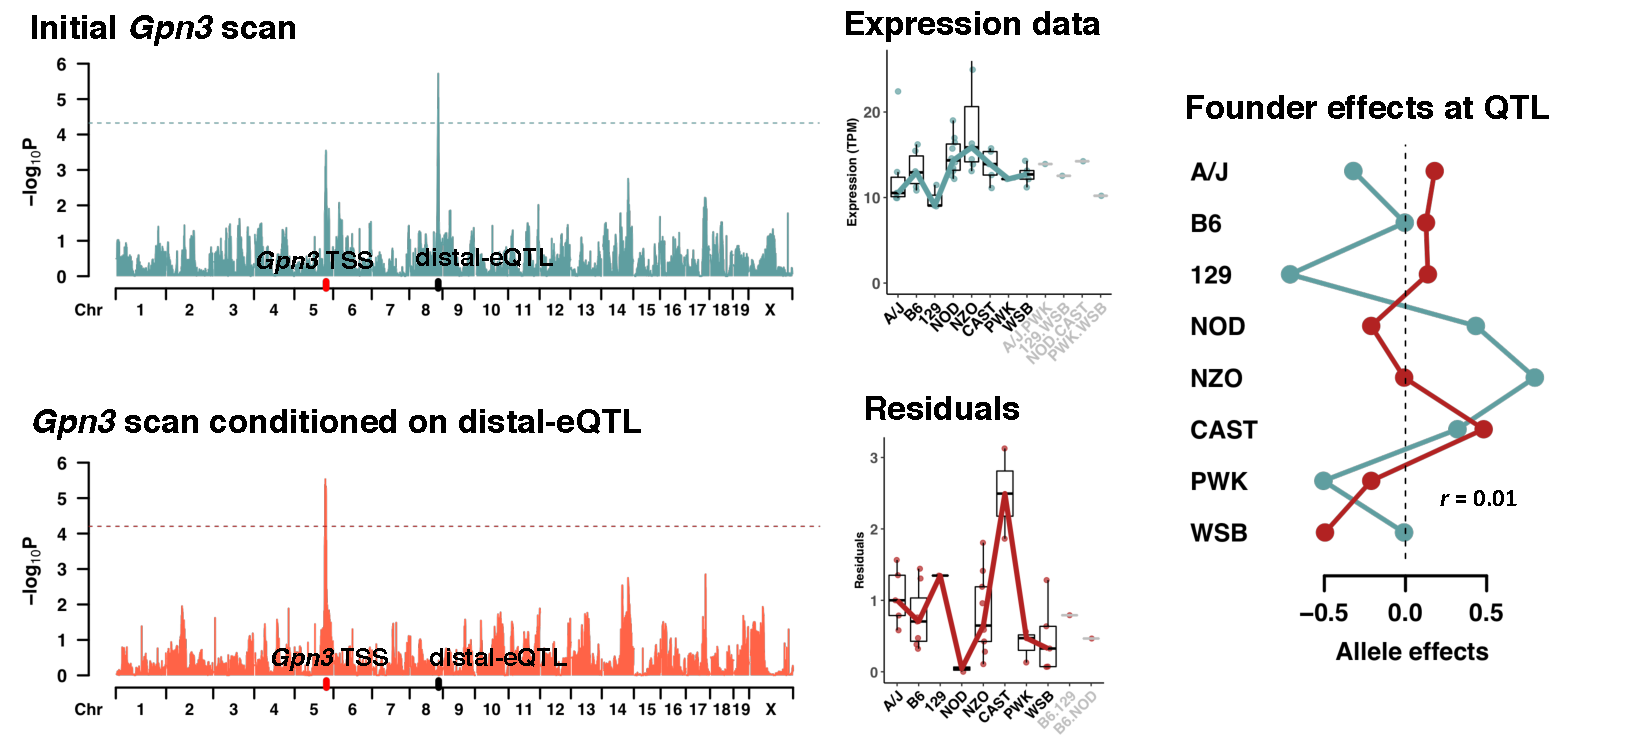
\includegraphics[width=\textwidth, trim={0in 0in 0in 0in}, clip]{figs/gpn3_conditional_scan.pdf}
\caption{\textbf{Detection of local-eQTL after conditioning on distal-eQTL for \textit{Gpn3}.} The multi-stage conditional regression approach of Method 1 allows for the detection of multiple genome-wide significant QTL, which can then be appropriately incorporated into a FDR procedure across many outcomes. In this example in lung tissue, the gene \textit{Gpn3} initially has a strong distal-eQTL on chromosome 8 (A). Though a peak is detected near the TSS of \textit{Gpn3}, it does not meet genome-wide significance. However, after conditioning on the distal-eQTL, the local-eQTL is detected (B). Horizontal dashed lines represent empirical 95\% significance thresholds based on 1000 permutations.
\label{fig:conditional_scans}}
\end{figure*}

\begin{figure*}[hp]
\renewcommand{\familydefault}{\sfdefault}\normalfont
\centering
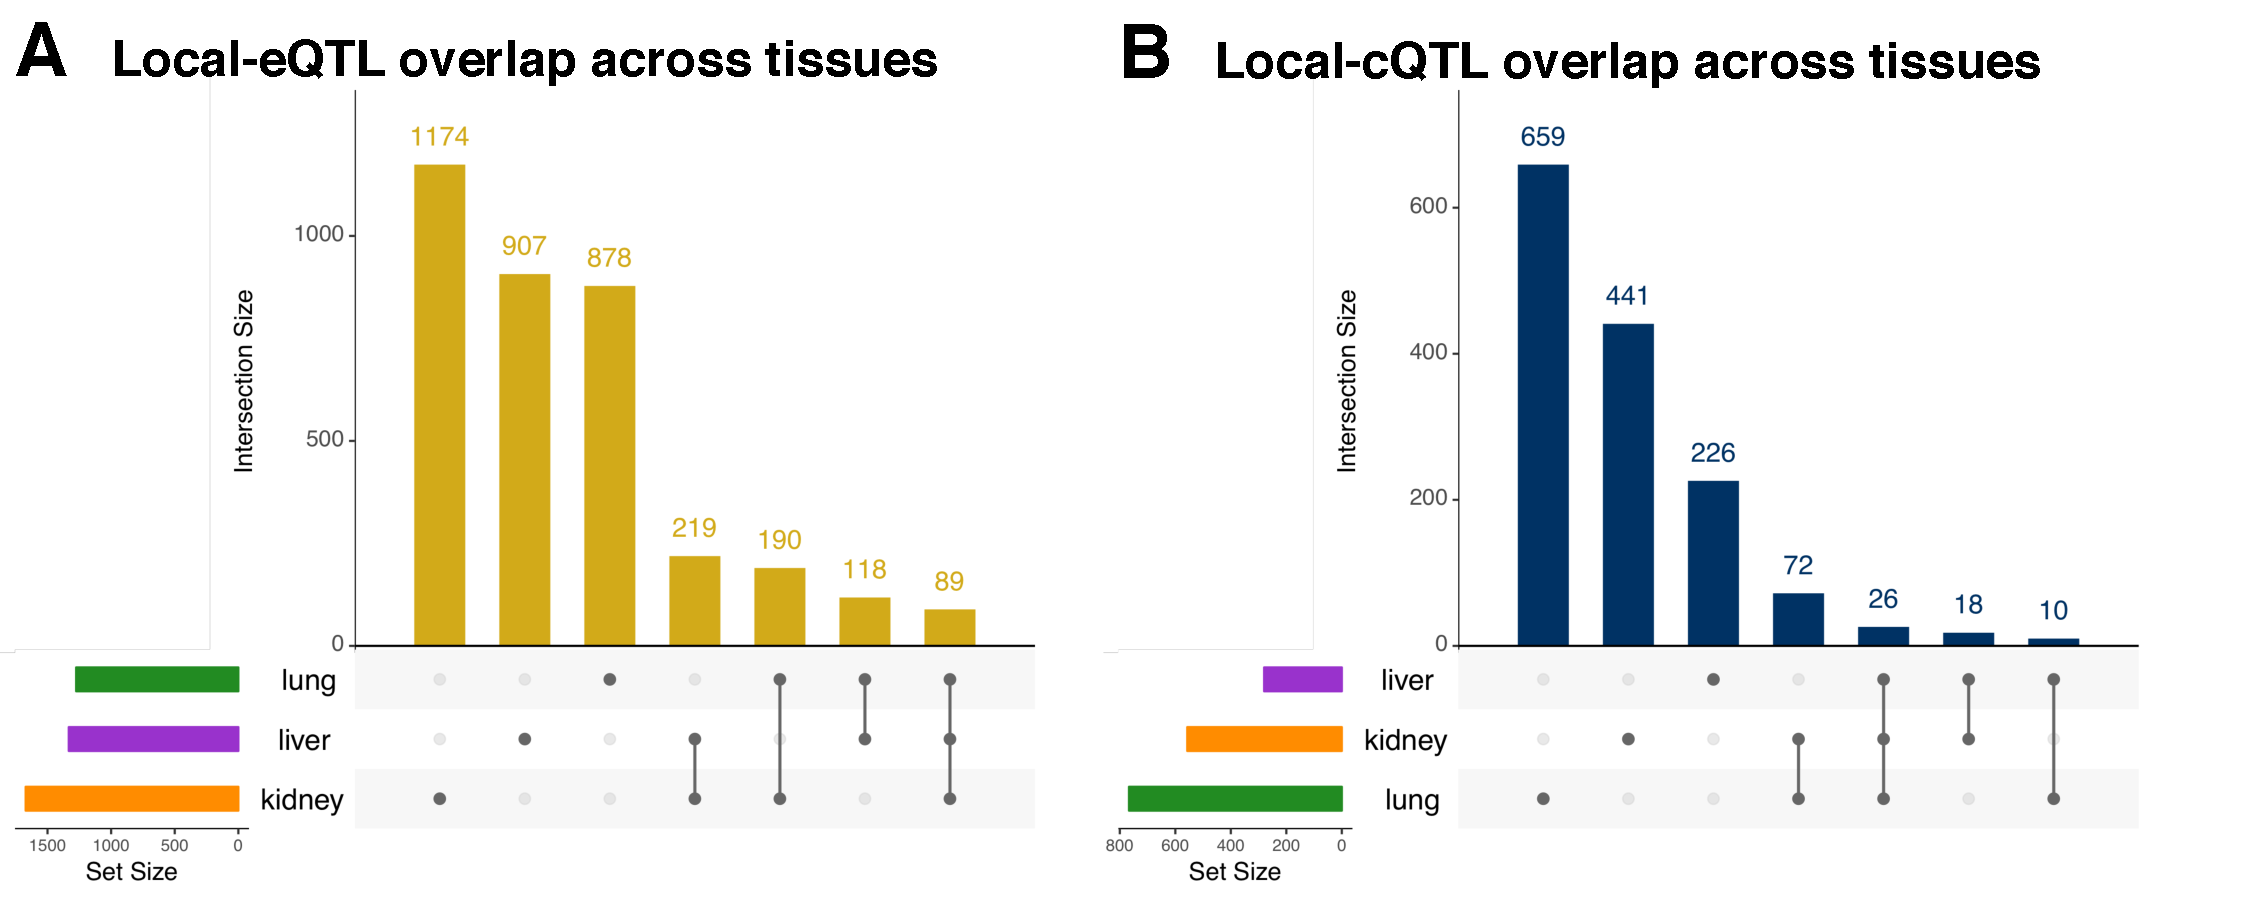
\includegraphics[width=\textwidth, trim={0in 0in 0in 0in}, clip]{figs/upset_eqtl_cqtl.pdf}
\caption{\textbf{Overlap across tissues of genes and chromatin windows with local-QTL detected.} The majority of sequence traits with a local-QTL detected were identified in only a single tissue. Kidney had the highest number of local-eQTL, whereas lung had the highest number of local-cQTL. Liver had a relative lack of local-cQTL, which may relate to its having the fewest chromatin windows analyzed (\textbf{Figure \ref{fig:upset_genes_chromatin} [right]}). Results included local-QTL detected with Method 1 (FDR < 0.1), Method 2 (FDR < 0.1), and Method 3 (genome-wide and chromosome-wide). 
\label{fig:upset_eqtl_cqtl}}
\end{figure*}

\begin{figure*}[h]
\renewcommand{\familydefault}{\sfdefault}\normalfont
\centering
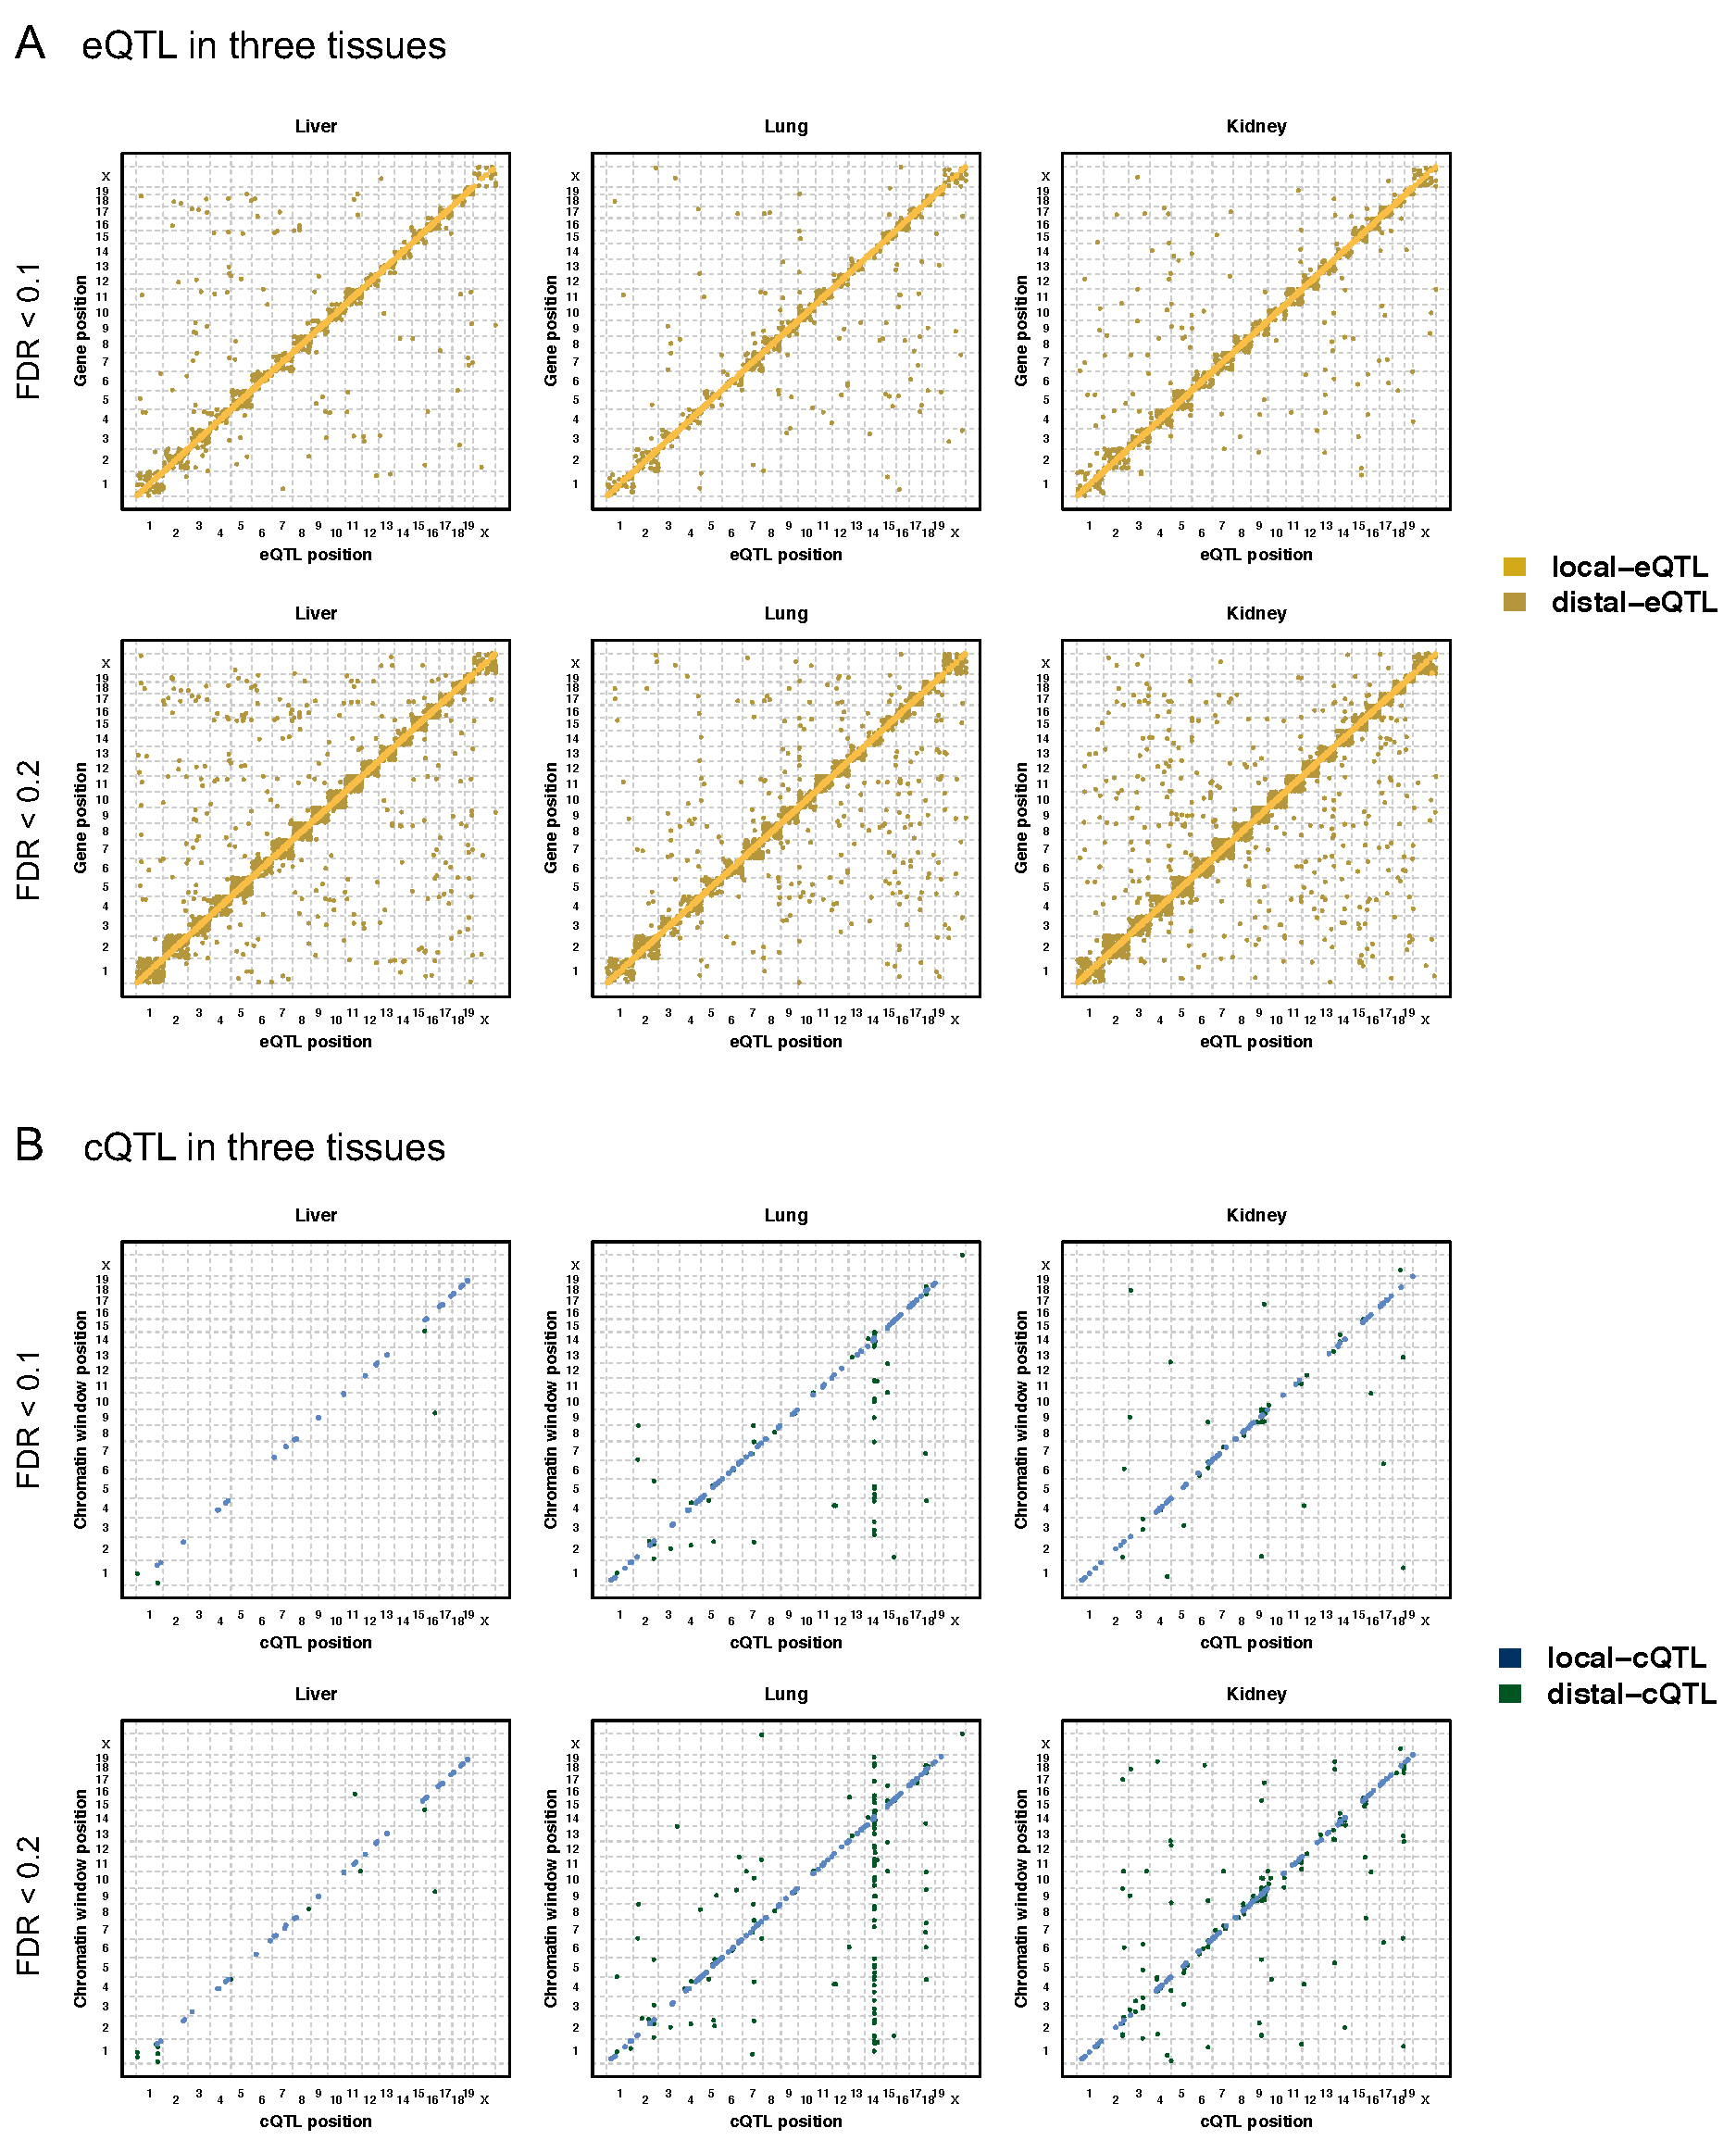
\includegraphics[width=0.8\textwidth, trim={0in 1.5in 0in 0in}, clip]{figs/qtl_map_supplemental.pdf}
\caption{\textbf{QTL mapping results using only Method 1 or Method 2.} QTL map plots of eQTL and cQTL with FDR controlled at 0.1 and 0.2 for liver, lung, and kidney. Detected QTL from Method 1 (multi-stage FDR) and Method 2 (chromosome-wide FDR) are included. Method 2, which uses FDR control for chromosome-wide significant QTL, produces a large number of intra-chromosomal distal QTL. The y-axis represents the genomic position of the gene or chromatin site, and the x-axis represents the genomic position of the QTL. Local-QTL appear as dots along the diagonal.
\label{fig:grid_fdr_plot}}
\end{figure*}

\begin{figure*}[h]
\centering
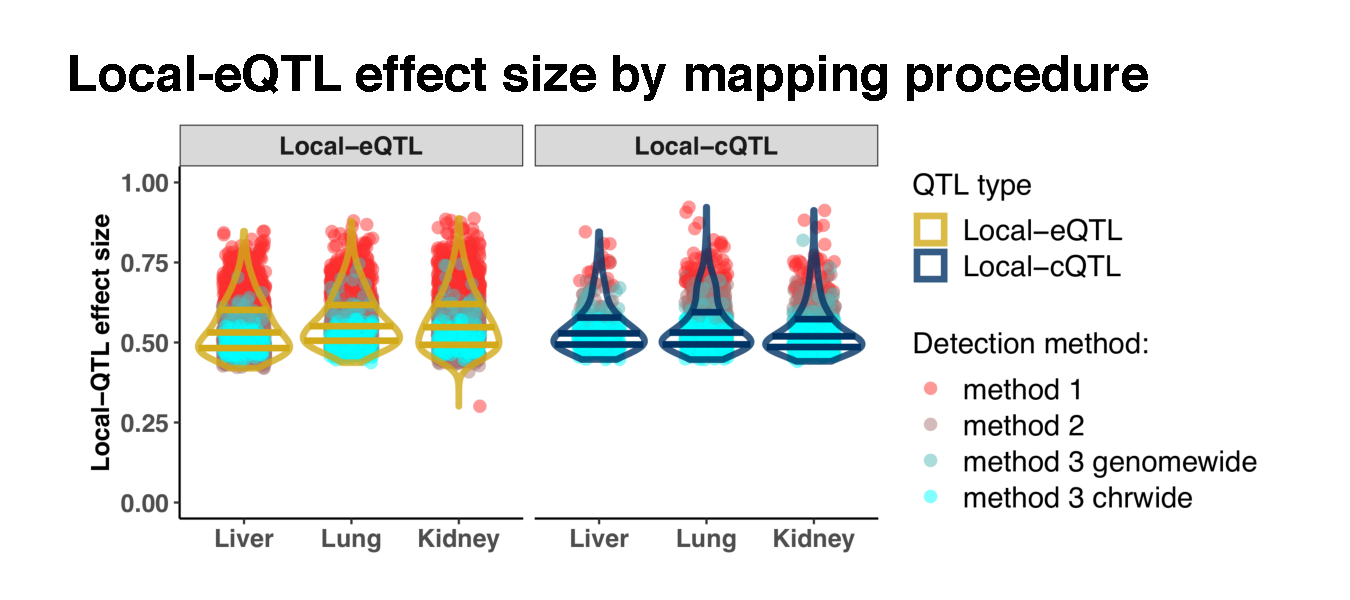
\includegraphics[width=\textwidth, trim={0in 0in 0in 0in}, clip]{figs/qtl_effect_size_by_method.pdf}
\caption{\textbf{Local-QTL effect sizes by mapping procedure.} Statistical procedures with greater rigor have reduced power to detect QTL of smaller effect sizes, shown in liver, lung, and kidney tissues for gene expression (yellow line) and chromatin accessibility (blue line). Each dot represents a detected local-QTL, colored according to the highest stringency mapping procedure that detected it. The three horizontal bars represent the 25\textsuperscript{th}, 50\textsuperscript{th}, and 75\textsuperscript{th} quantiles of QTL effect sizes for all local-QTL per tissue. The multi-stage genome-wide FDR (Method 1) generally detects QTL with effect size > 30\%, whereas the chromosome-wide FDR (Method 2), and FWER-adjusted p-values (permP; Method 3), genome-wide or chromosome-wide can detect QTL effect sizes > 15\%. Effect size estimates correspond to a fixed effects model of the QTL (Eq \ref{eq:effect_size}).
\label{fig:qtl_effect_sizes_by_method}}
\end{figure*}

\begin{figure*}[h]
\centering
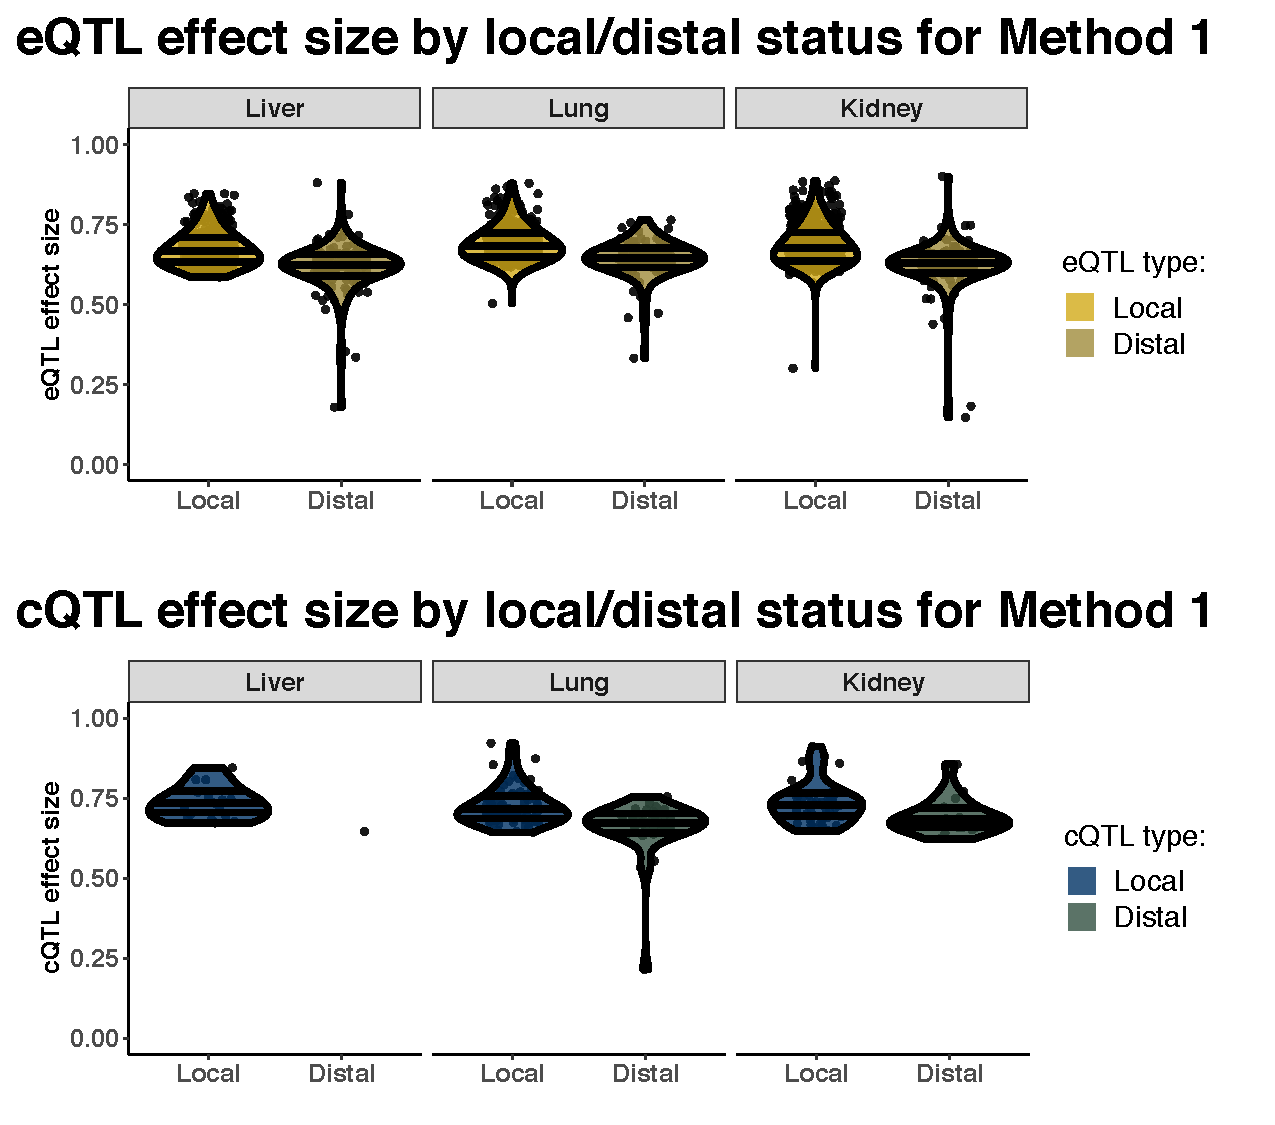
\includegraphics[width=0.9\textwidth, trim={0in 0in 0in 0in}, clip]{figs/qtl_effect_sizes_strict.pdf}
\caption{\textbf{QTL effect sizes by local/distal status for Method 1.} Each dot represents a detected QTL through either Method 1 (FDR $\leq$ 0.1). The three horizontal bars represent the 25\textsuperscript{th}, 50\textsuperscript{th}, and 75\textsuperscript{th} quantiles of QTL effect sizes for all local-QTL per tissue. More local-QTL are detected and have larger effects on average than the detected distal-QTL, in both gene expression and chromatin accessibility. Effect size estimates are based on a fixed effects model (Eq \ref{eq:effect_size}).
\label{fig:qtl_effect_sizes_strict}}
\end{figure*}

\begin{figure*}[h]
\centering
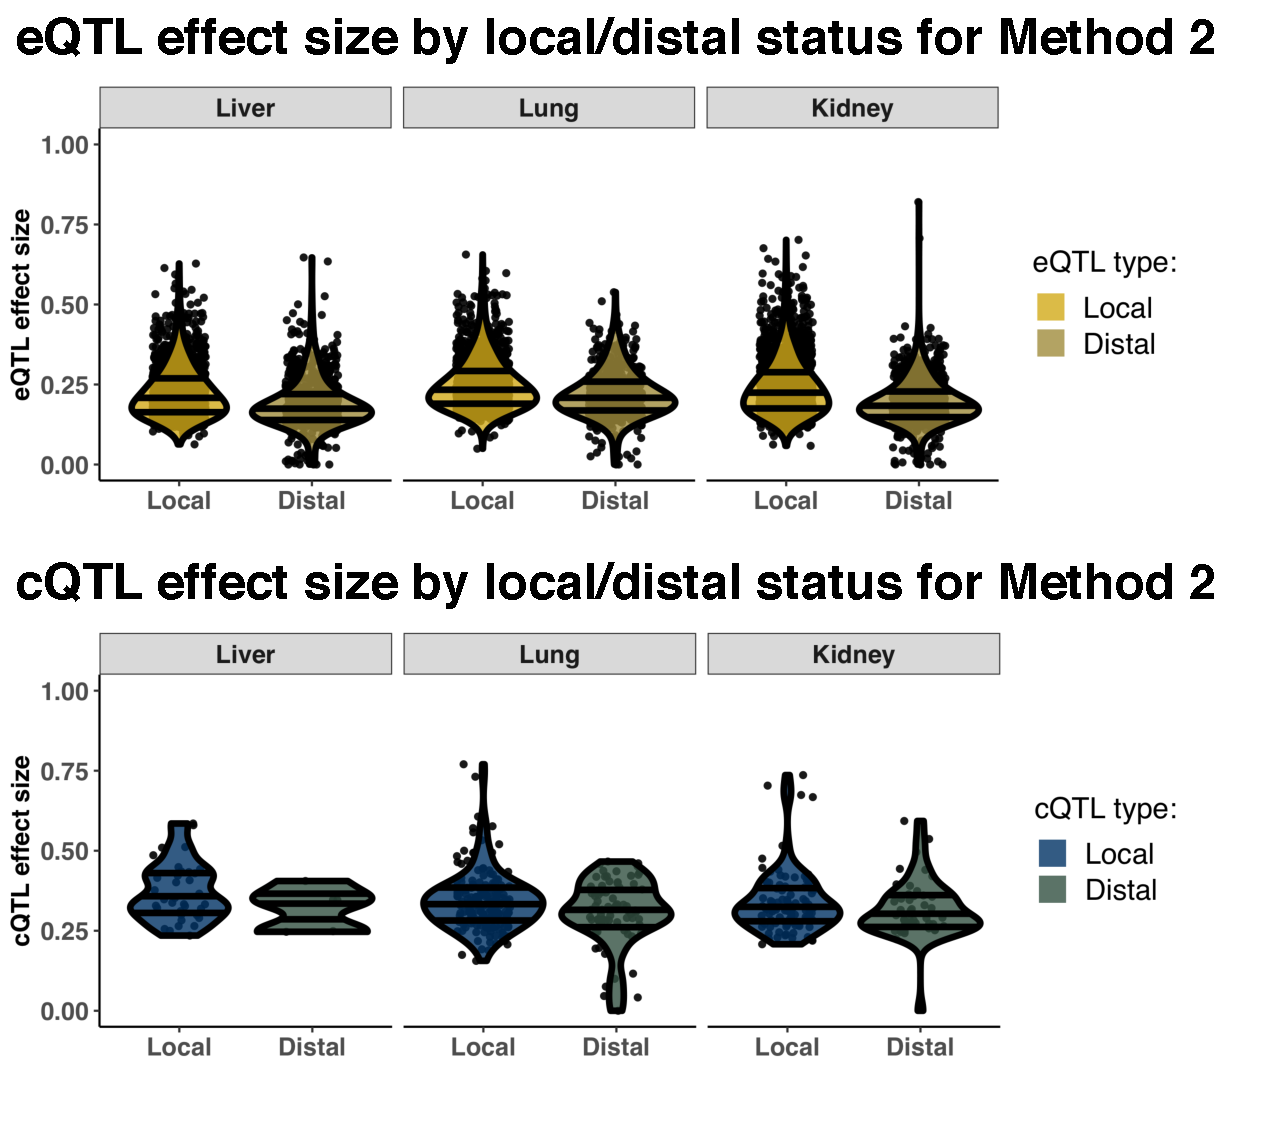
\includegraphics[width=0.9\textwidth, trim={0in 0.25in 0in 0in}, clip]{figs/qtl_effect_sizes_permissive.pdf}
\caption{\textbf{QTL effect sizes by local/distal status for Methods 1 and 2.} Each dot represents a QTL detected through either Method 1 or Method 2 (FDR $\leq$ 0.1). The three horizontal bars represent the 25\textsuperscript{th}, 50\textsuperscript{th}, and 75\textsuperscript{th} quantiles of QTL effect sizes for all local-QTL per tissue. Consistent with Method 1 results, more local-eQTL are detected and have higher effects than distal-QTL. Method 2 detects a large number of intra-chromosomal distal-QTL that Method 1 does not, many of which have low effect sizes. Effect size estimates are based on a fixed effects model (Eq \ref{eq:effect_size}).
\label{fig:qtl_effect_sizes_permissive}}
\end{figure*}

\begin{figure*}[h]
\centering
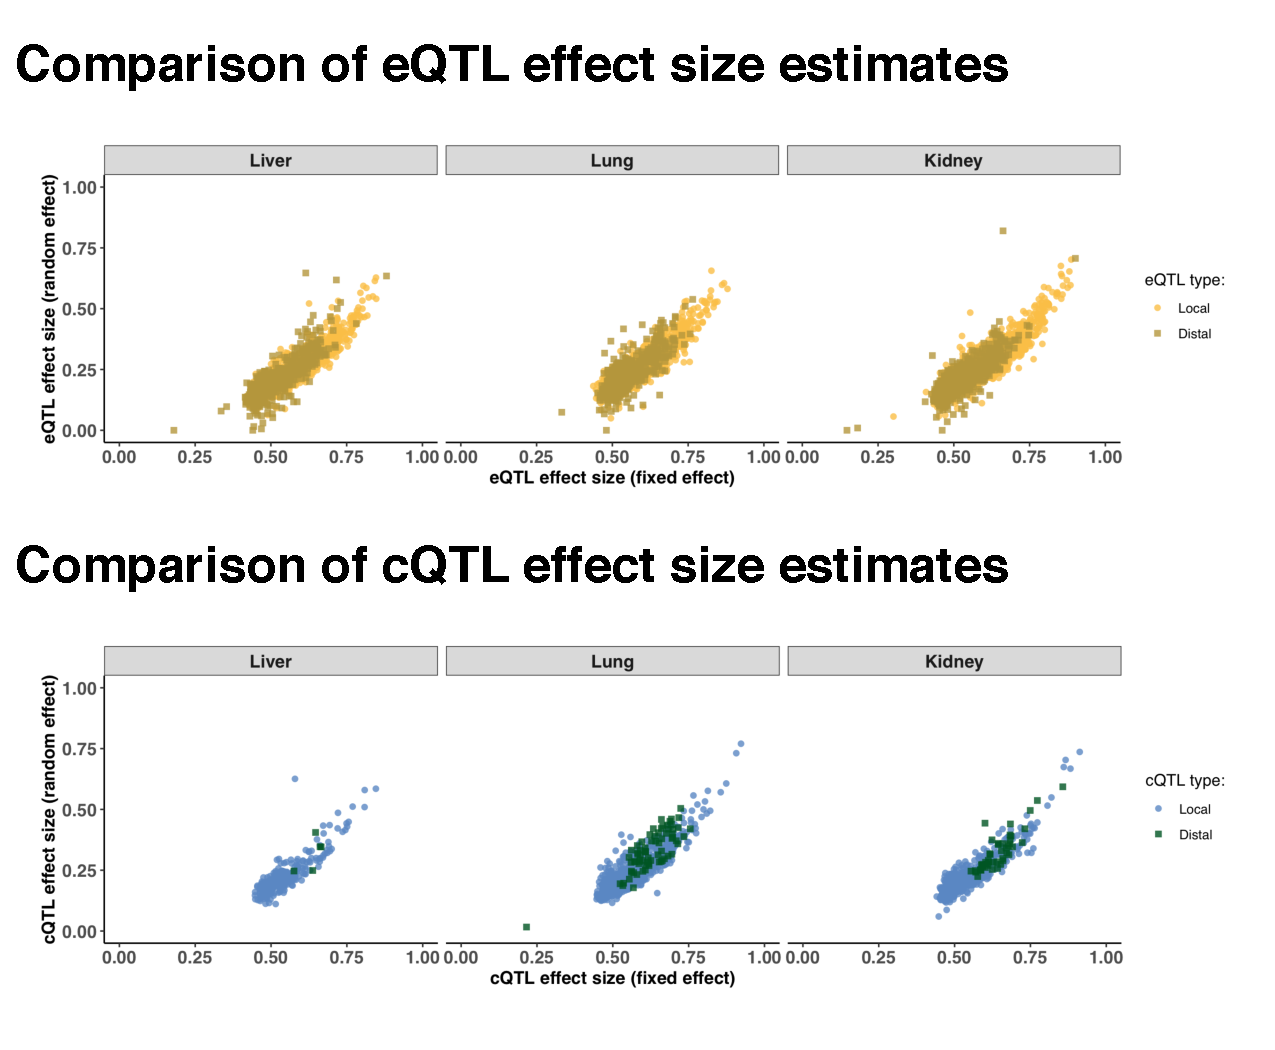
\includegraphics[width=0.9\textwidth, trim={0in 0in 0in 0in}, clip]{figs/fixefvsranef_qtl.pdf}
\caption{\textbf{Comparison of QTL effect sizes estimates from fixed effects and random effects models.} The effect size corresponding to the random effect fit (Y-axis; Eq \ref{eq:effect_size_ranef}) is harshly penalized compared to the fixed effect estimate (X-axis; Eq \ref{eq:effect_size}), likely due to a small sample size of 47 individuals. Notably, there are a number of distal-eQTL that are more harshly reduced by the random effects model compared to the other QTL, likely representing signals resulting from extreme observations or imbalances in founder contributions at the locus. QTL detected by Methods 1 (FDR $\le 0.1$), 2 (FDR $\le 0.1$), and 3 are shown.
\label{fig:qtl_effect_size_fixefvsranef}}
\end{figure*}

\begin{figure*}[hp]
\renewcommand{\familydefault}{\sfdefault}\normalfont
\centering
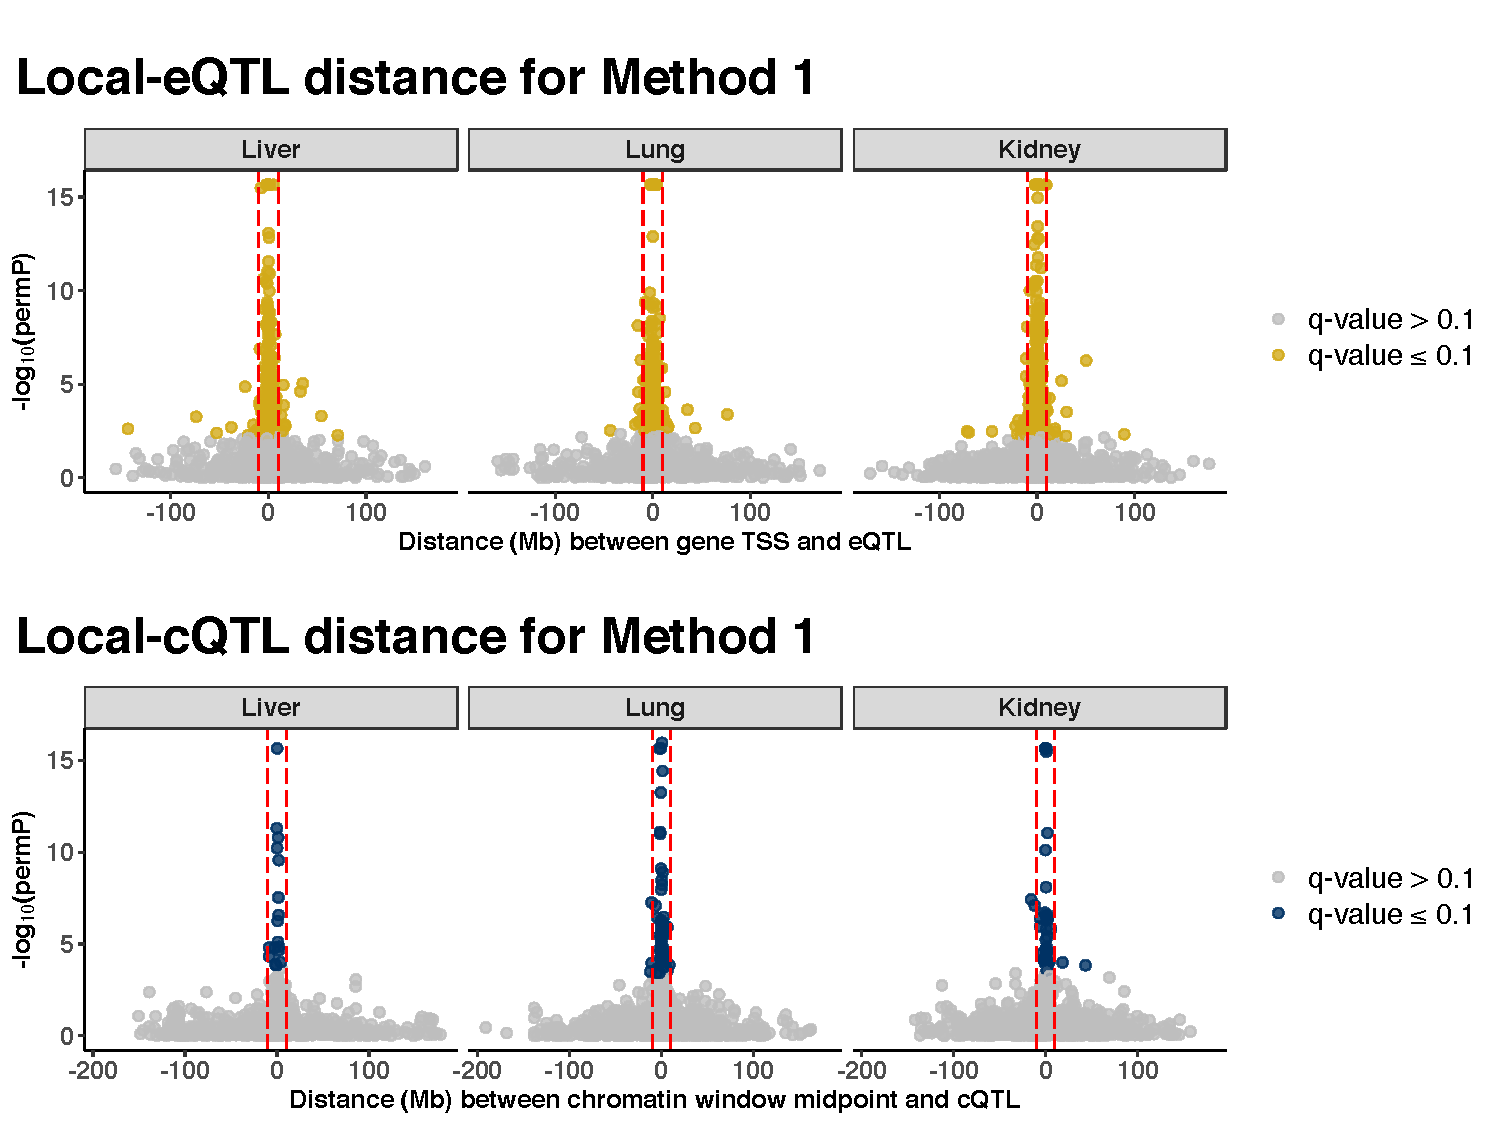
\includegraphics[width=0.9\textwidth]{figs/qtl_distance_method1.pdf}
\caption{\textbf{Highly significant QTL are proximal to gene TSS and chromatin window midpoint.} The genome-wide permutation-based p-value (permP) from Method 1 (first stage-only) for eQTL and cQTL compared to the distance (Mb) from the gene TSS and the midpoint of the chromatin site, respectively. Inter-chromosomal distal-QTL are not included. The red dashed lines represent 10 Mb upstream and downstream of the gene TSS or the midpoint of the chromatin site for classifying QTL as local or distal. Significant signals (yellow or blue), based on $\text{q-value} \le 0.1$, are largely local. \label{fig:genomewide_dist}}
\end{figure*}

\begin{figure*}[hp]
\renewcommand{\familydefault}{\sfdefault}\normalfont
\centering
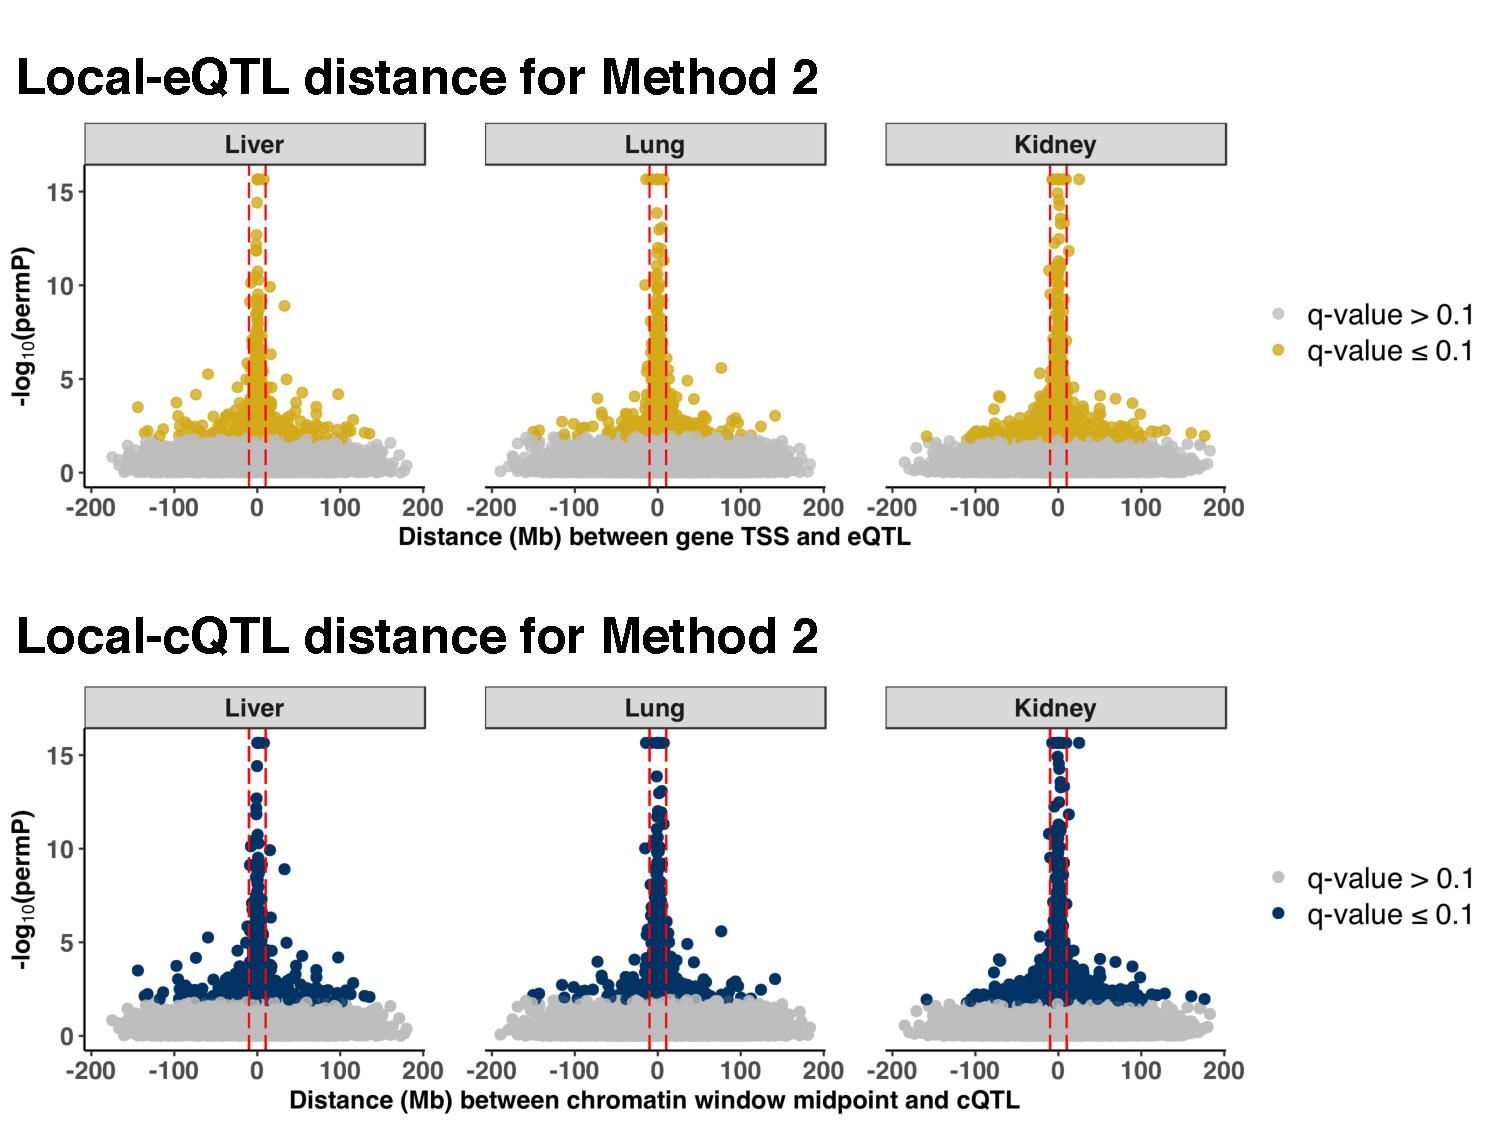
\includegraphics[width=0.9\textwidth]{figs/qtl_distance_method2.pdf}
\caption{\textbf{Methods that use chromosome-wide significance detect many putative intra-chromosomal distal-QTL.} The chromosome-wide permutation-based p-value (permP) from Method 2 for eQTL and cQTL compared to distance (Mb) from the gene TSS and the midpoint of the chromatin site, respectively. Method 2 is restricted to QTL on the local-chromosome. The red dashed lines represent 10 Mb upstream and downstream of gene TSS or chromatin site for classifying an association as local or distal. Significant QTL (yellow or blue) are largely proximal.
\label{fig:chrwide_dist}}
\end{figure*}

\begin{figure*}[hp]
\renewcommand{\familydefault}{\sfdefault}\normalfont
\centering
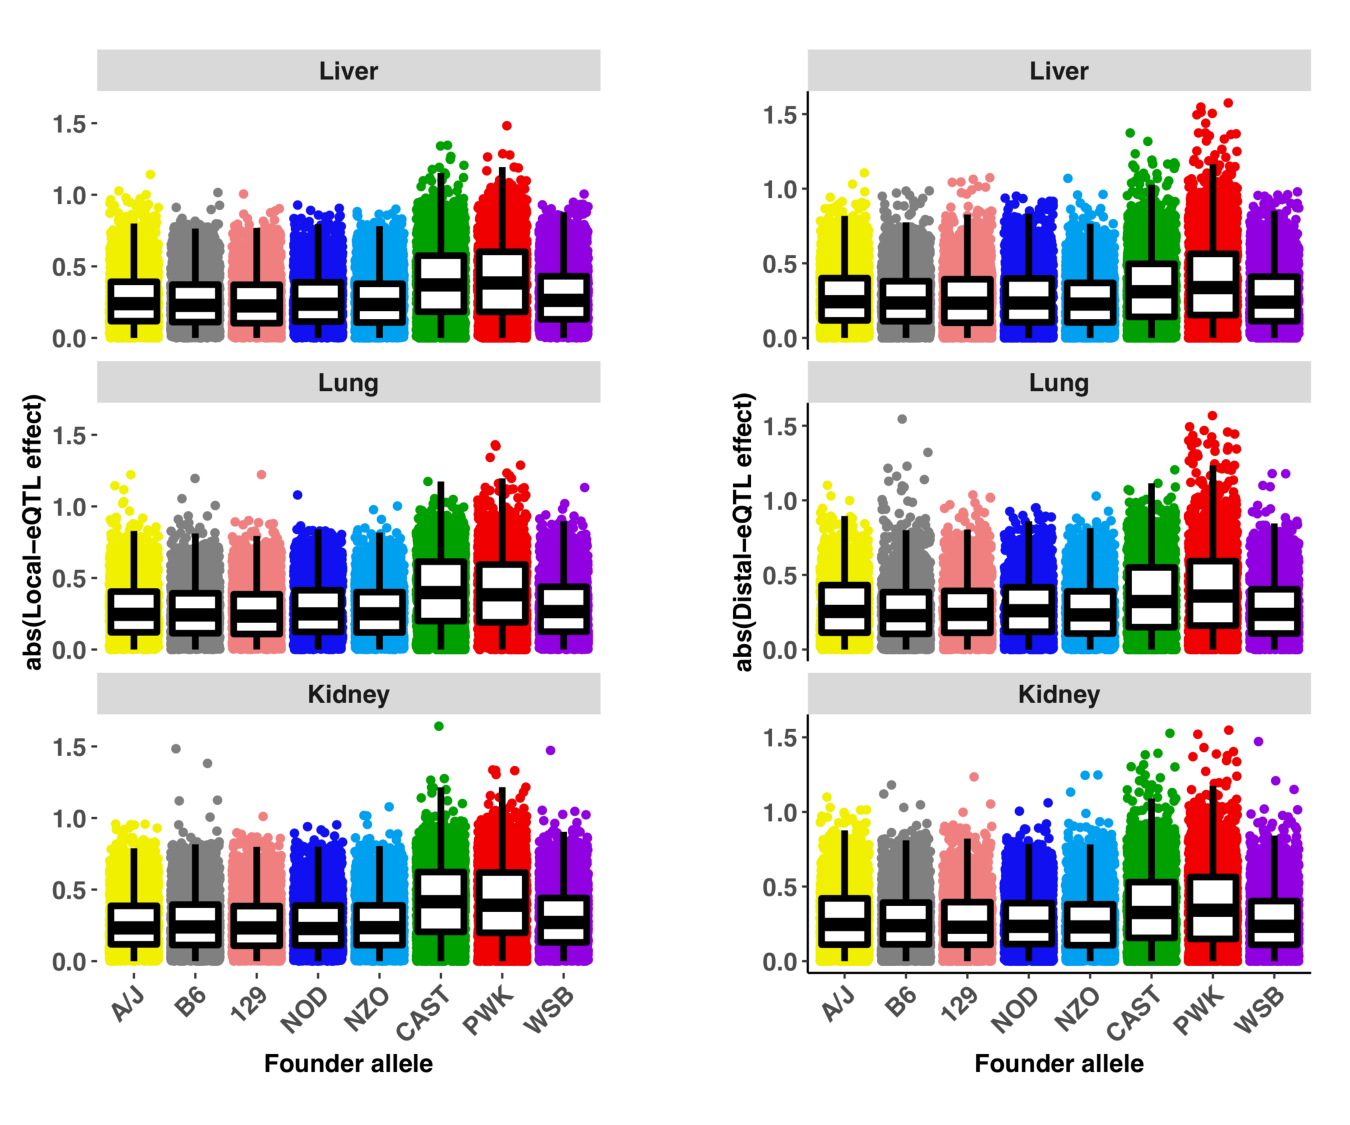
\includegraphics[width=\textwidth, trim={0in 0in 0in 0in}, clip]{figs/all_eqtl_effects_abs.pdf}
\caption{\textbf{CAST and PWK alleles have more extreme effects for eQTL than the other strains.} Founder strain effects were estimated by fitting the QTL effect as a random effect in the model from Eq \ref{eq:alternative_model}, thus representing constrained BLUPs. Each eQTL represents an 8-element effect vector. The founders effects by definition are centered around 0. Taking the absolute value allows for a comparison of the relative magnitudes, allowing for the identification of founders that produce more extreme effects on average. Founder effects for cQTL are displayed in \textbf{Figure \ref{fig:cqtl_effects_abs}}.
\label{fig:eqtl_effects_abs}}
\end{figure*}

\begin{figure*}[hp]
\renewcommand{\familydefault}{\sfdefault}\normalfont
\centering
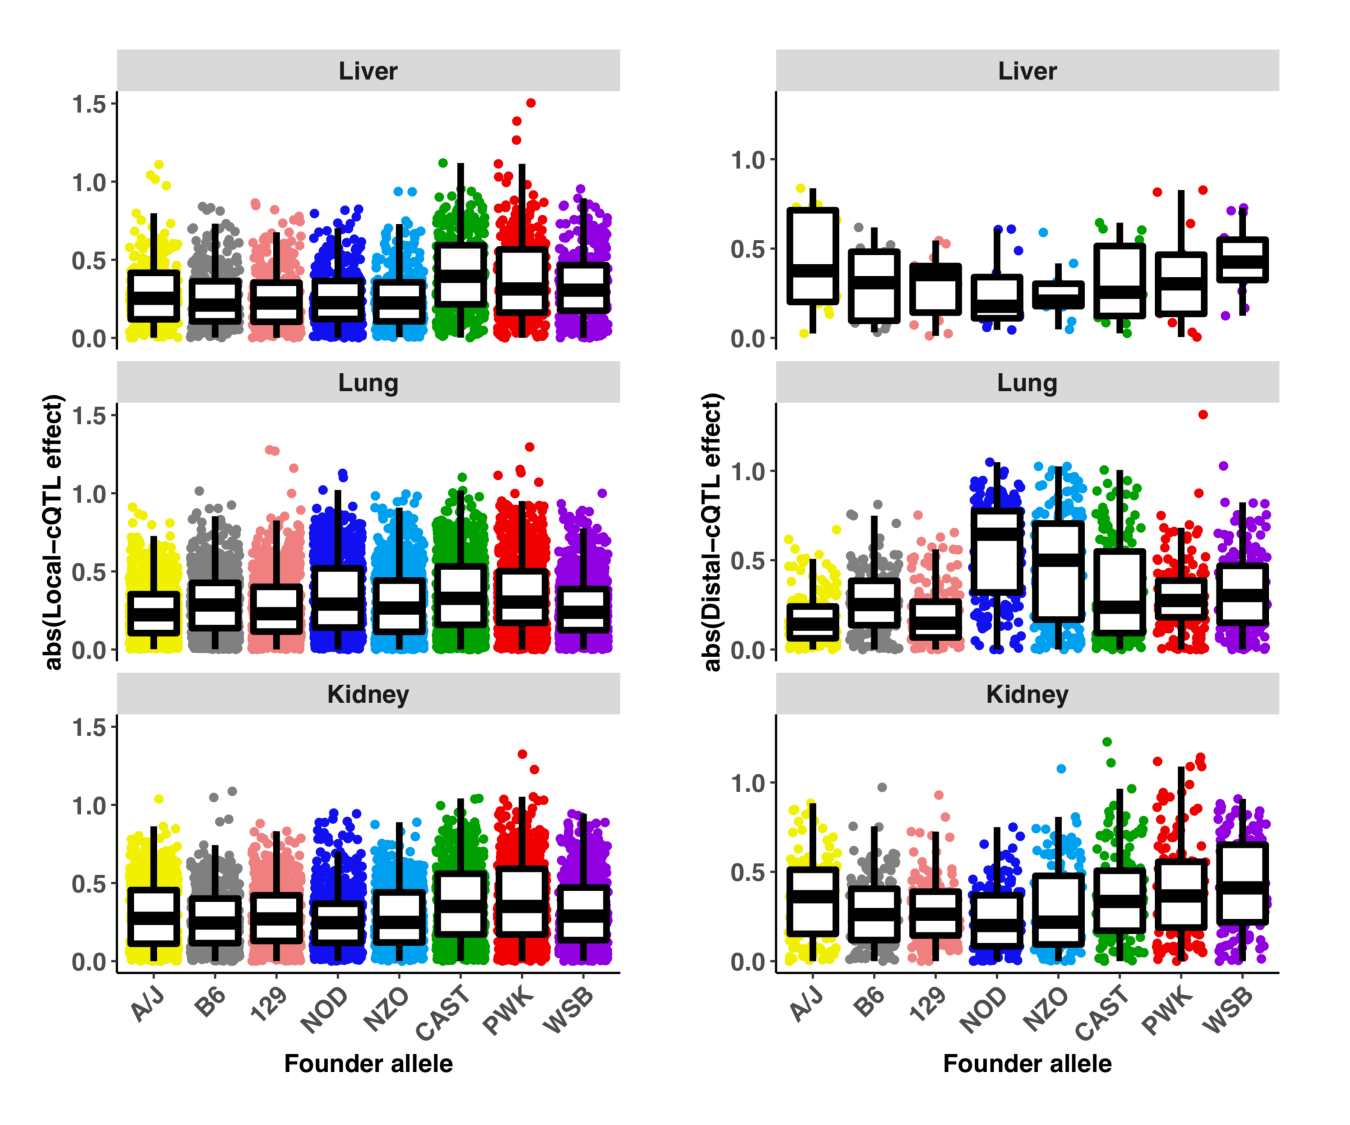
\includegraphics[width=\textwidth, trim={0in 0in 0in 0in}, clip]{figs/all_cqtl_effects_abs.pdf}
\caption{\textbf{CAST and PWK alleles have more extreme effects for cQTL than the other strains.} Using a random effects model to fit the QTL effect in Eq \ref{eq:alternative_model}, founder effects were estimated as BLUPs, which are constrained and centered around 0. Each cQTL is represented by an 8-element effect vector. Founders with on average more extreme effects are identified by comparing the absolute values of effects. Founder effects for eQTL are in \textbf{Figure \ref{fig:eqtl_effects_abs}}, which are similar to cQTL but better represented.
\label{fig:cqtl_effects_abs}}
\end{figure*}

\begin{figure*}[hp]
\renewcommand{\familydefault}{\sfdefault}\normalfont
\centering
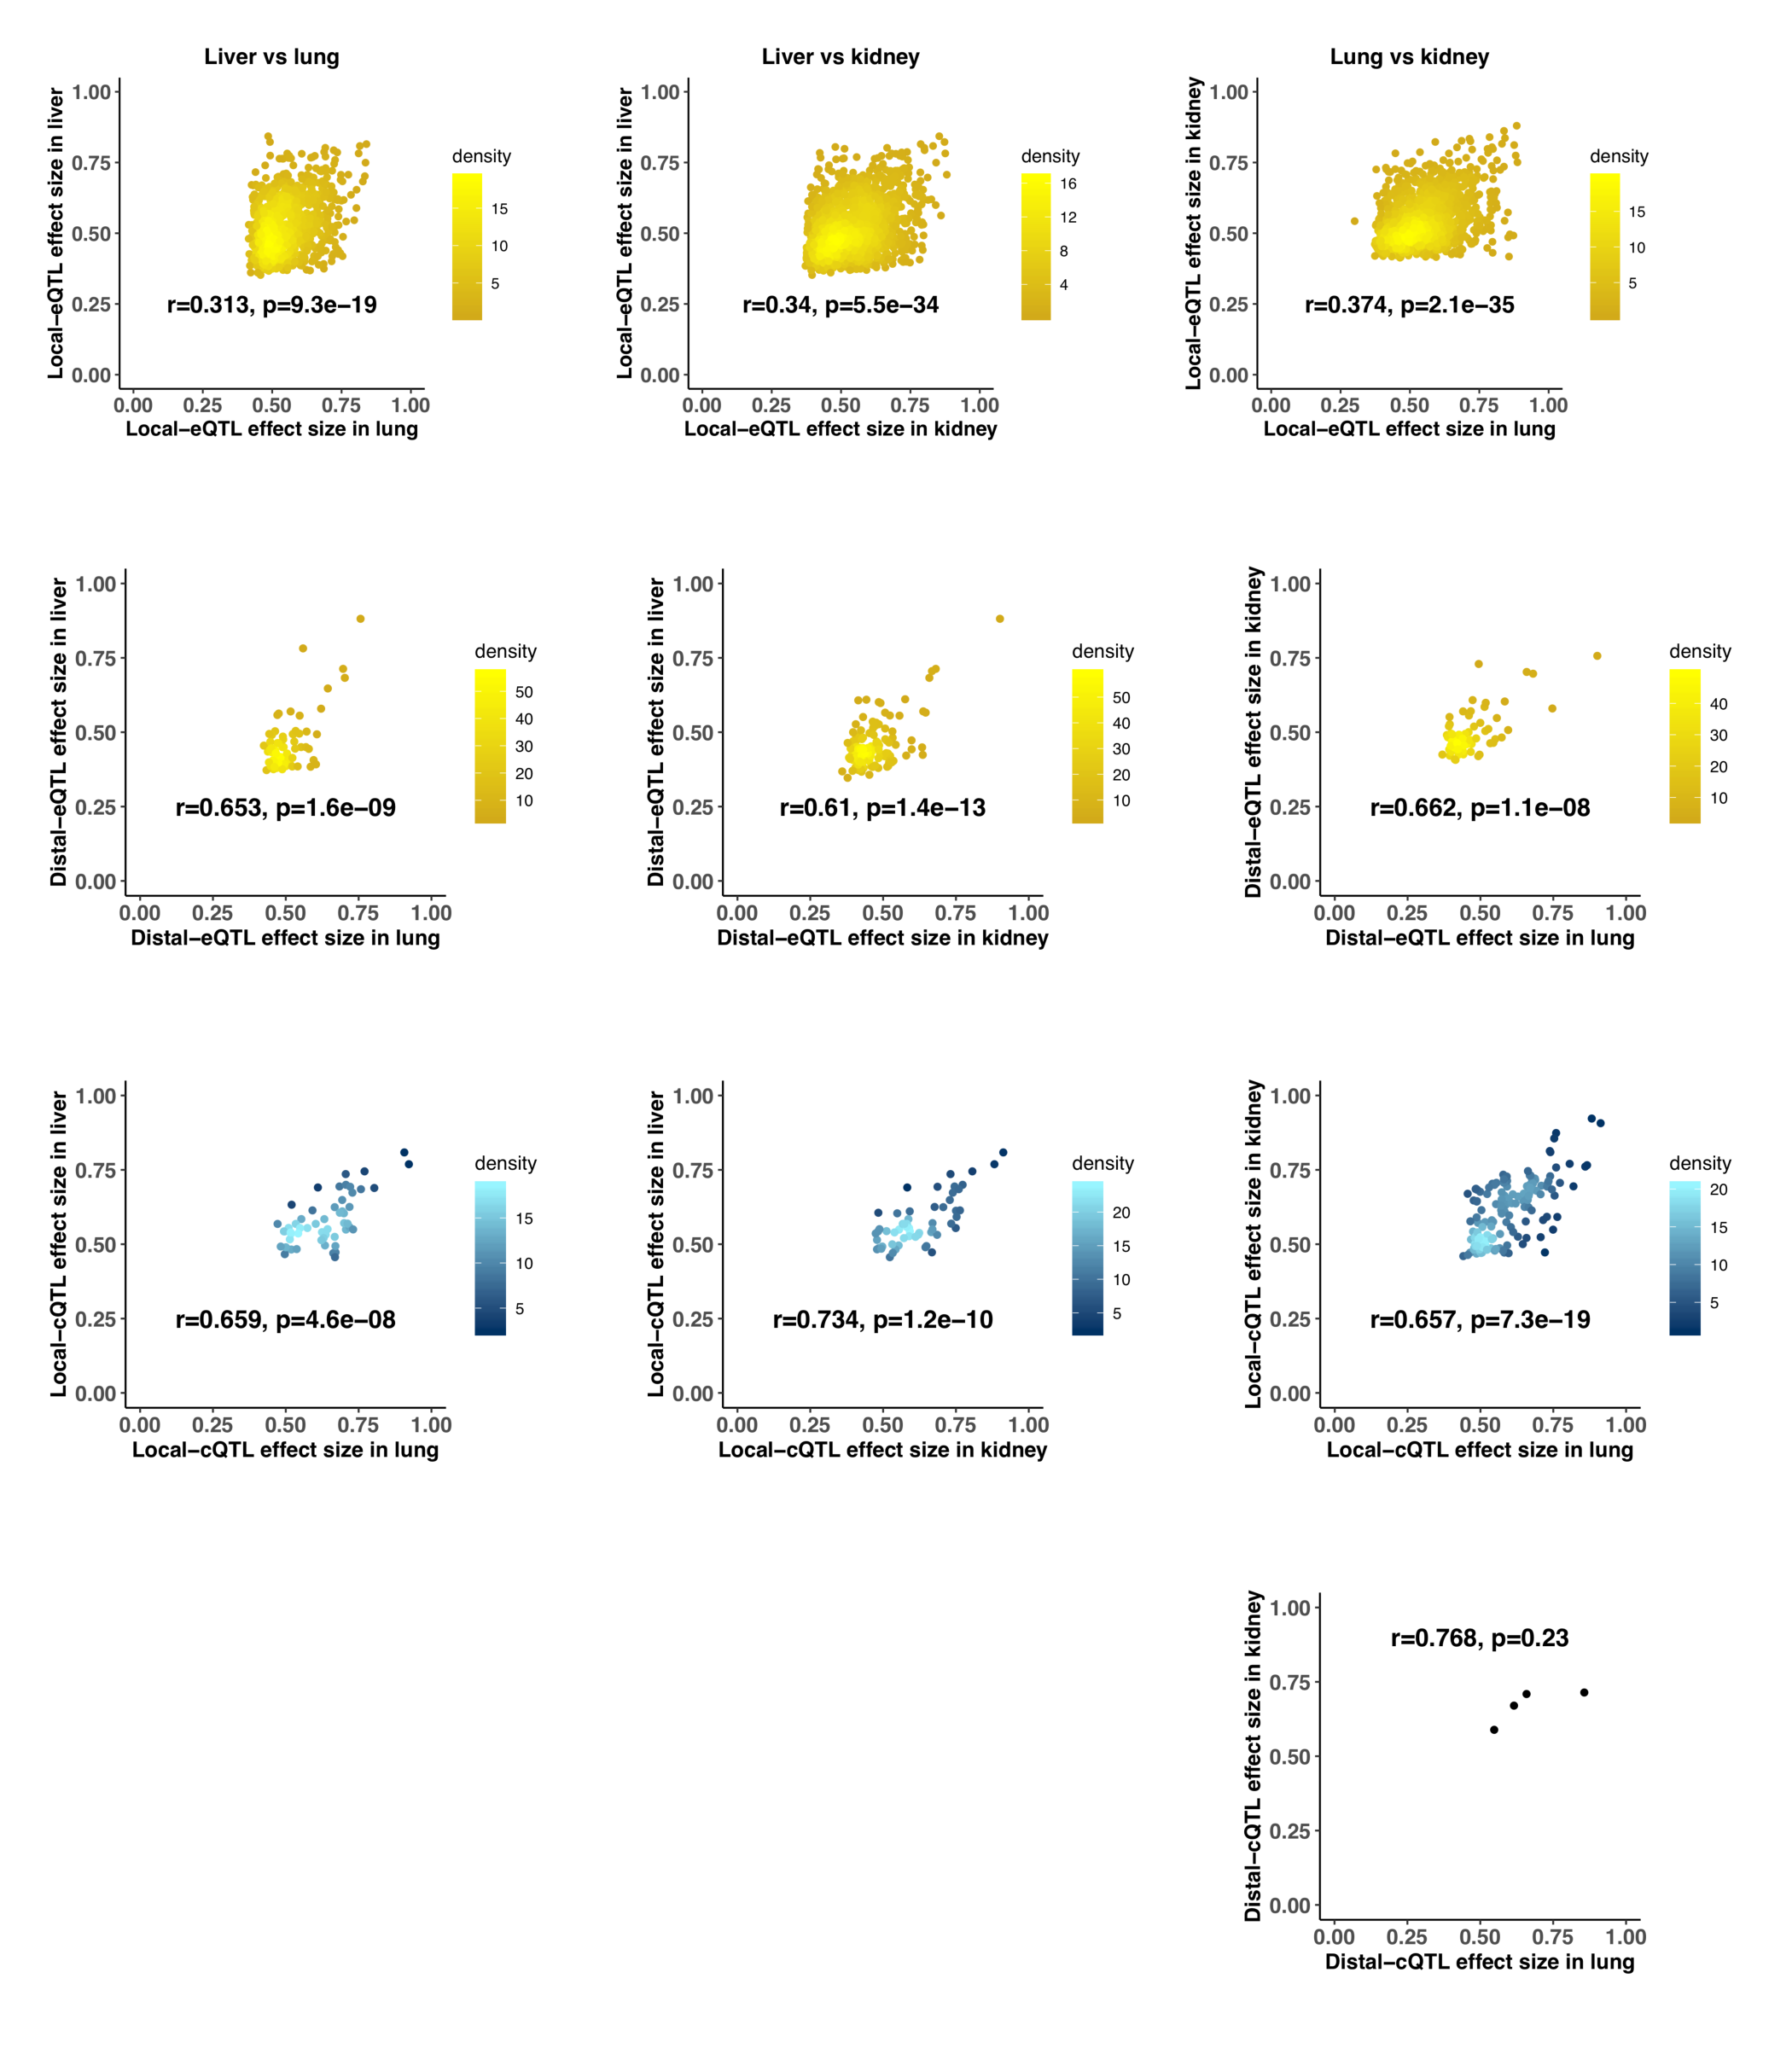
\includegraphics[width=0.9\textwidth, trim={0in 0in 0in 0in}, clip]{figs/effect_size_by_effect_size.pdf}
\caption{\textbf{Effect sizes between QTL pairs are lowly but significantly correlated.} Comparisons of QTL effects sizes, calculated according to Eq \ref{eq:effect_size}, between (liver/lung) are in the left column, (liver/kidney) middle column, and (lung/kidney) right column. eQTL are yellow and cQTL are blue. Local-eQTL are plotted in the top row, distal-eQTL in the second row, local-cQTL in the third row, and distal-cQTL in the bottom row, with only four pairs detected in (lung/kidney). 
\label{fig:qtl_effect_size_comparison}}
\end{figure*}

\begin{figure*}[hp]
\renewcommand{\familydefault}{\sfdefault}\normalfont
\centering
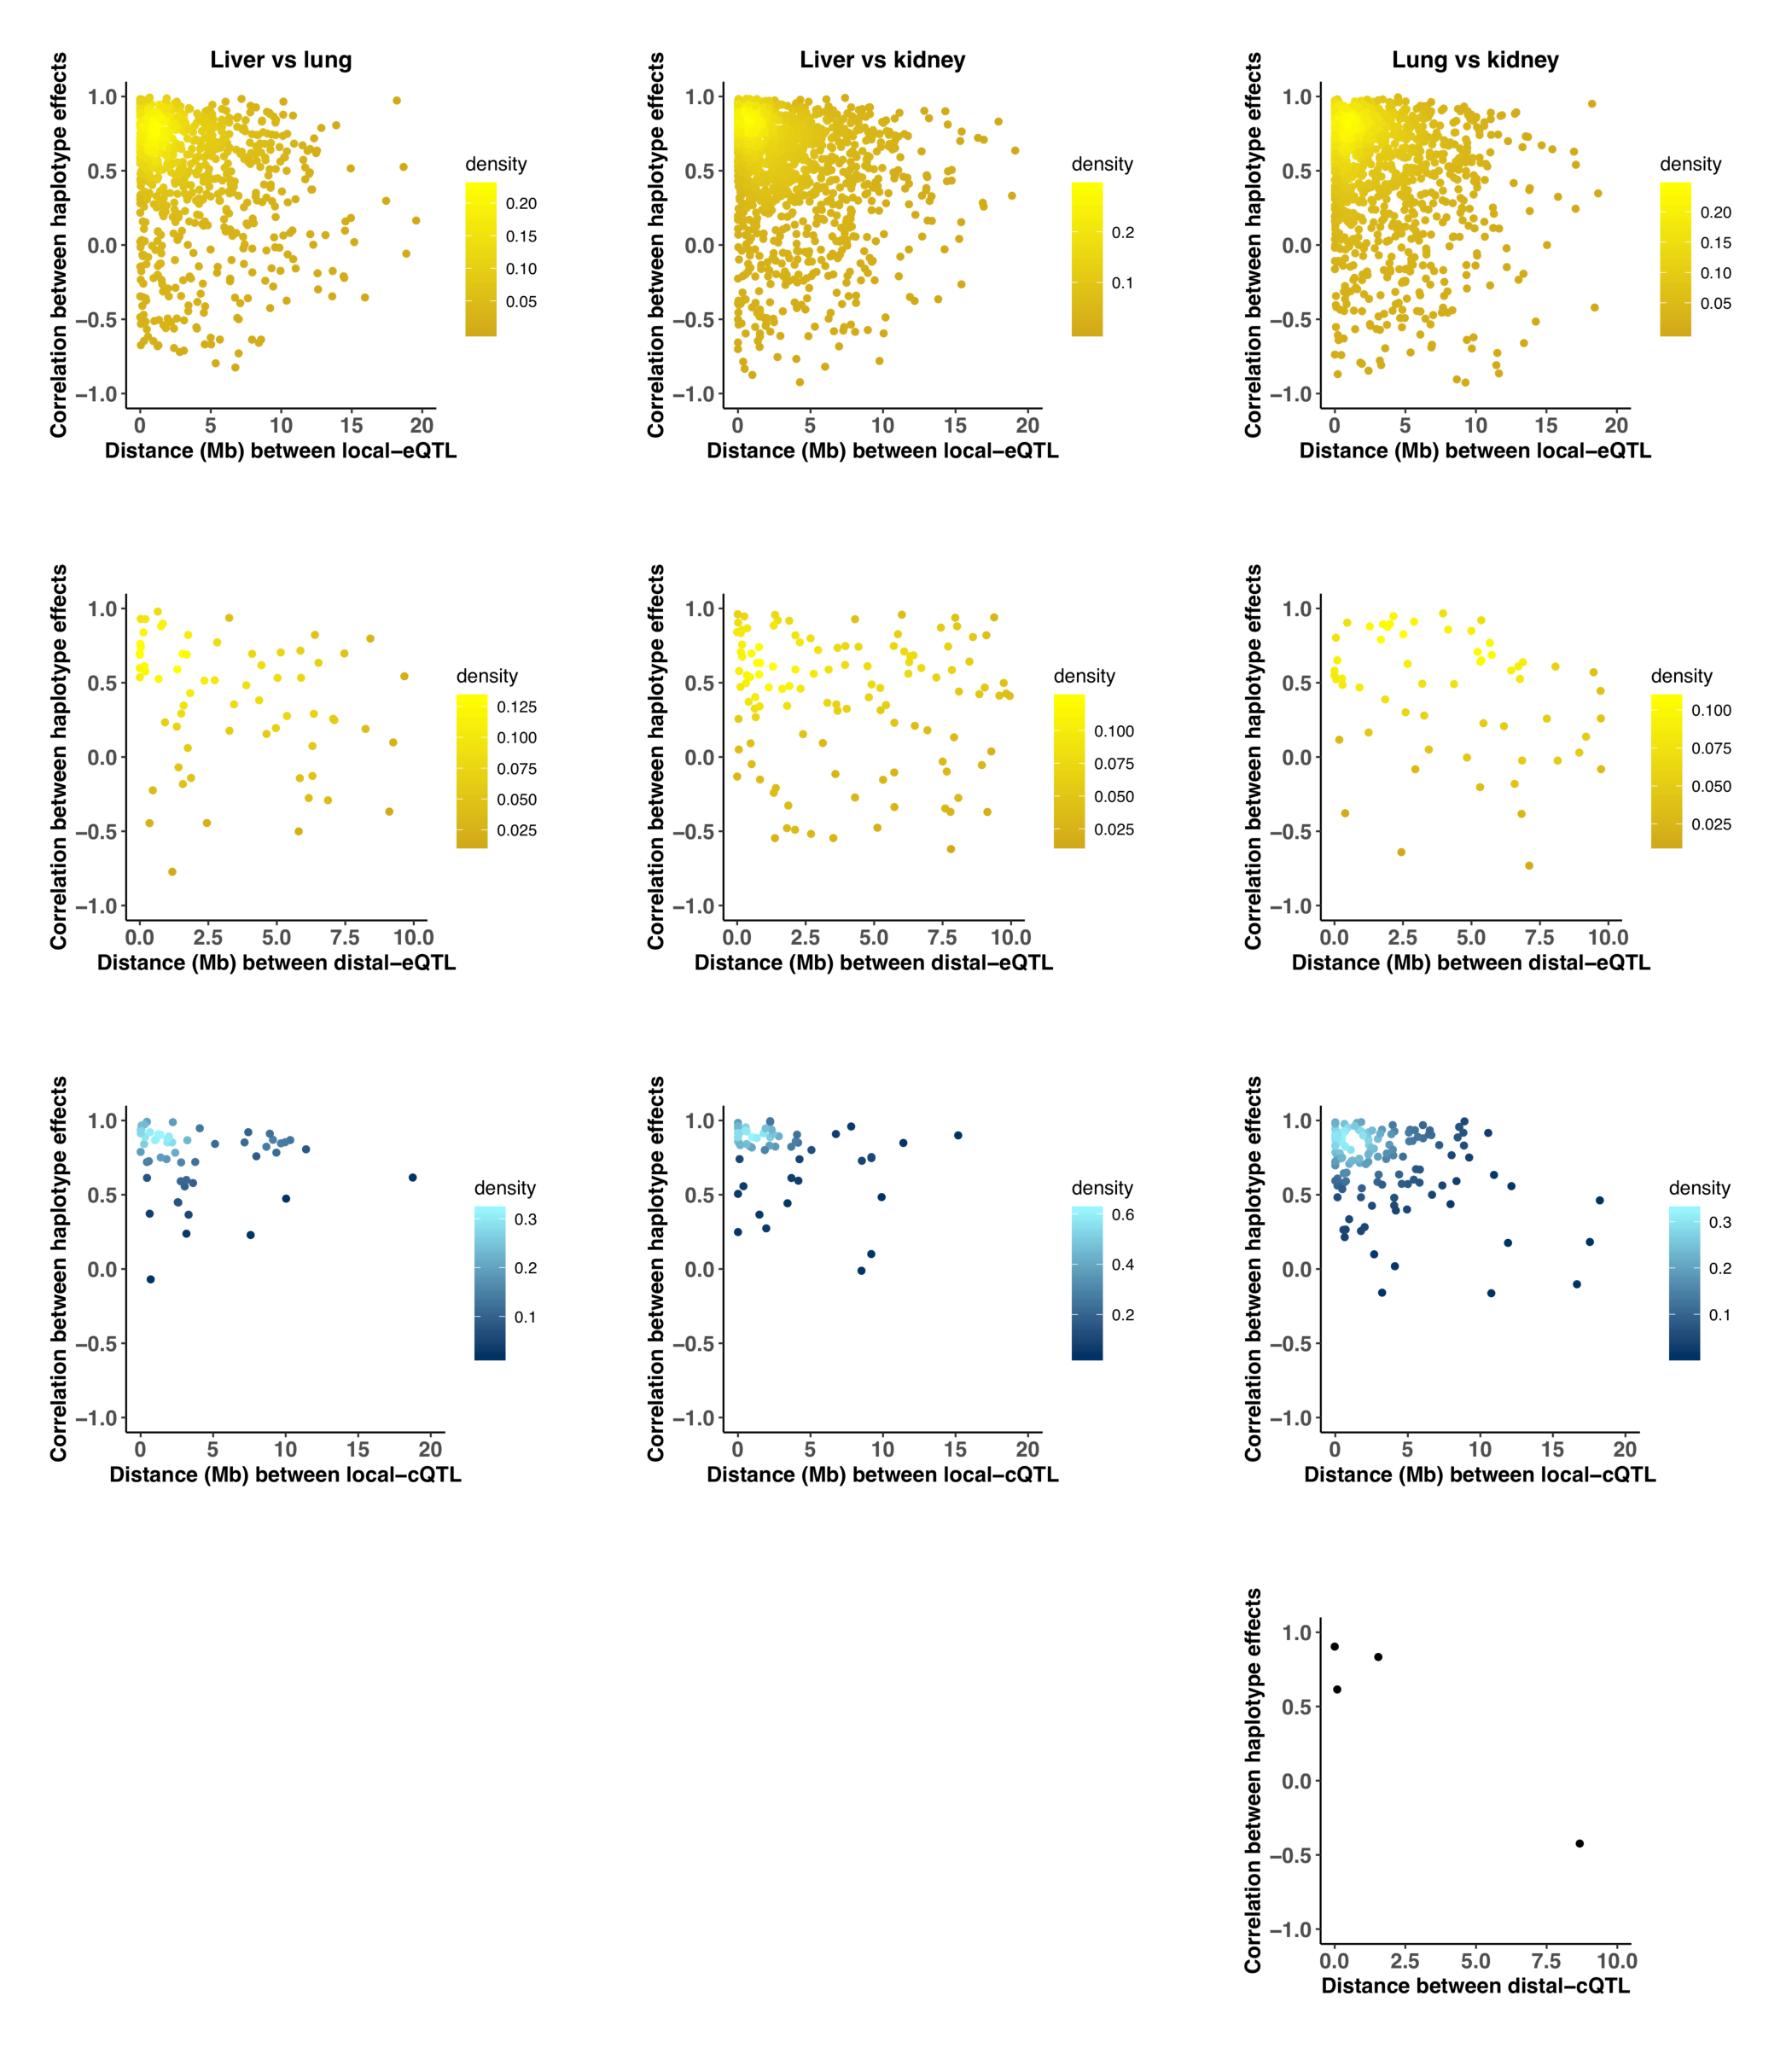
\includegraphics[width=0.9\textwidth, trim={0in 0in 0in 0in}, clip]{figs/effect_size_cor_by_dist.pdf}
\caption{\textbf{QTL pairs with highly correlated founder allele effects map proximally to each other.} Founder effects were estimated as constrain BLUPs. Pairwise correlations of the 8-element effect vectors were calculated for QTL pairs, and plotted again the distance between the QTL coordinates in Mb for (liver/lung) in the left column, (liver/kidney) in the middle column, and (lung/kidney) in the right column. Single eQTL and cQTL pairs are represented as a yellow and blue dots, respectively. Local-eQTL are shown in the top row, distal-eQTL in the second row, local-cQTL in the third row, and distal c-QTL in the bottom row, for which only four pairs were detected in (lung/kidney).
\label{fig:qtl_cor_by_distance_comparison}}
\end{figure*}

\begin{figure*}[hp]
\renewcommand{\familydefault}{\sfdefault}\normalfont
\centering
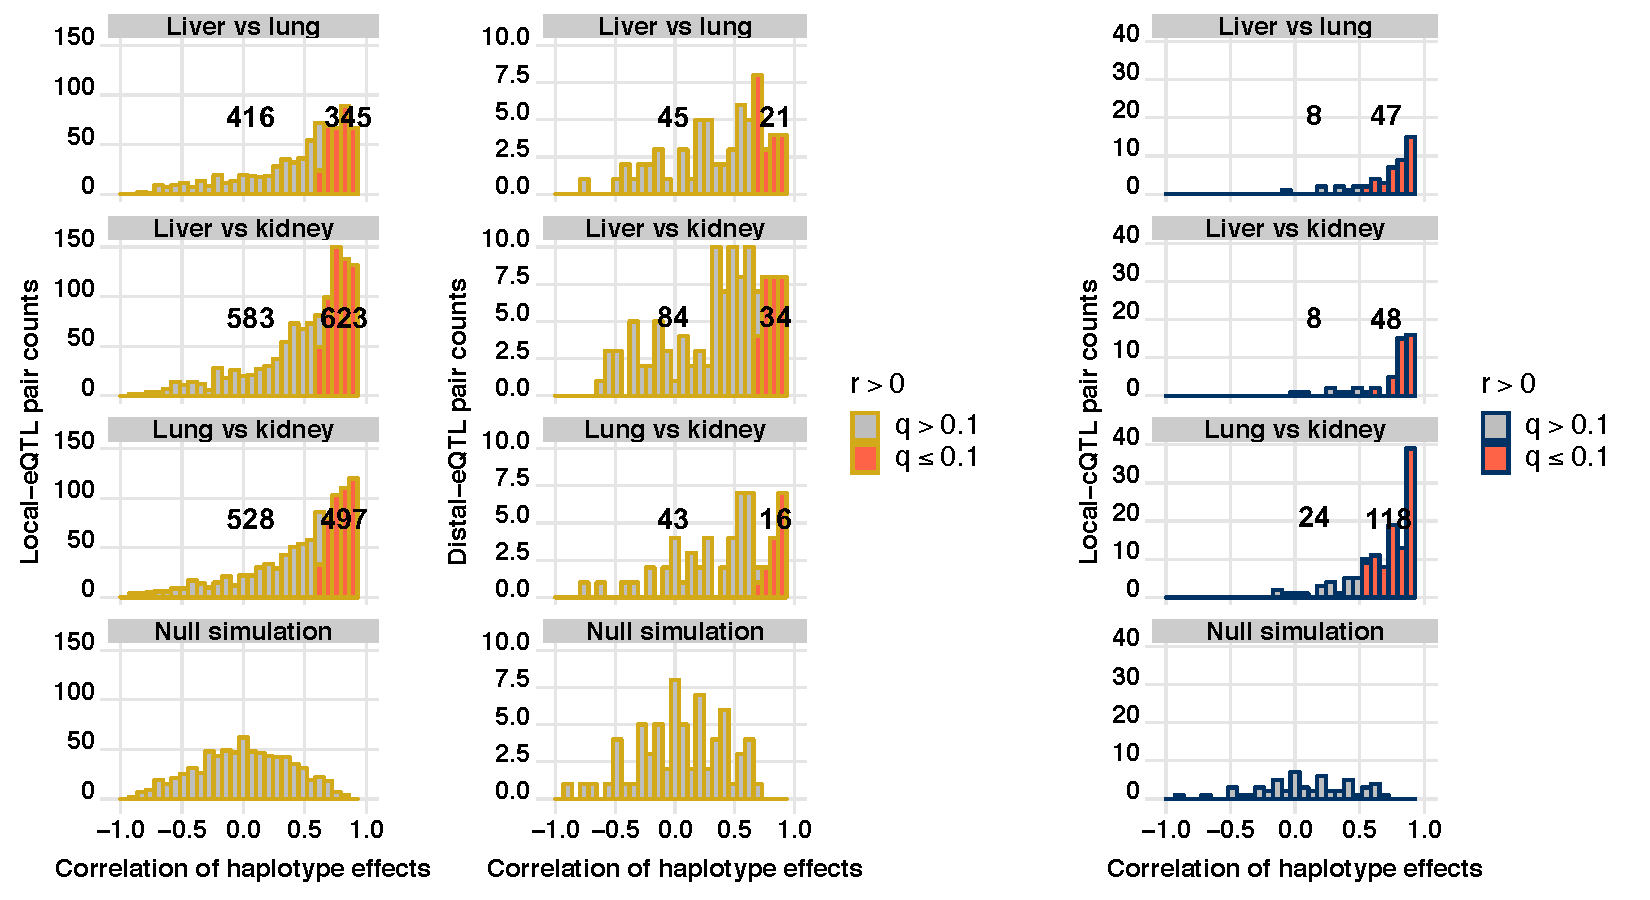
\includegraphics[width=\textwidth, trim={0in 0in 0in 0in}, clip]{figs/qtl_pair_cor_histograms.pdf}
\caption{\textbf{Consistent genetic regulation of gene expression and chromatin accessibility observed across tissues.} Enrichment of significantly correlated founder allele effects detected in QTL pairs for gene expression and chromatin accessibility. Pairs of QTL observed in multiple tissues were defined for local-eQTL (left column), distal-eQTL (middle column), and local-cQTL (right column). Only four pairs of distal-cQTL were observed, all shared between lung and kidney. A right-tailed test the correlation between founders effects ($H_{A}: r > 0$) was performed for each QTL pair, producing p-values that were then FDR adjusted. Null simulations of uncorrelated 8-element vector pairs for each class of QTL and pairwise tissue comparison emphasize the observed enrichment in correlated founder effects between QTL pairs.  
\label{fig:qtl_pair_histograms}}
\end{figure*}

\begin{figure*}[hp]
\renewcommand{\familydefault}{\sfdefault}\normalfont
\centering
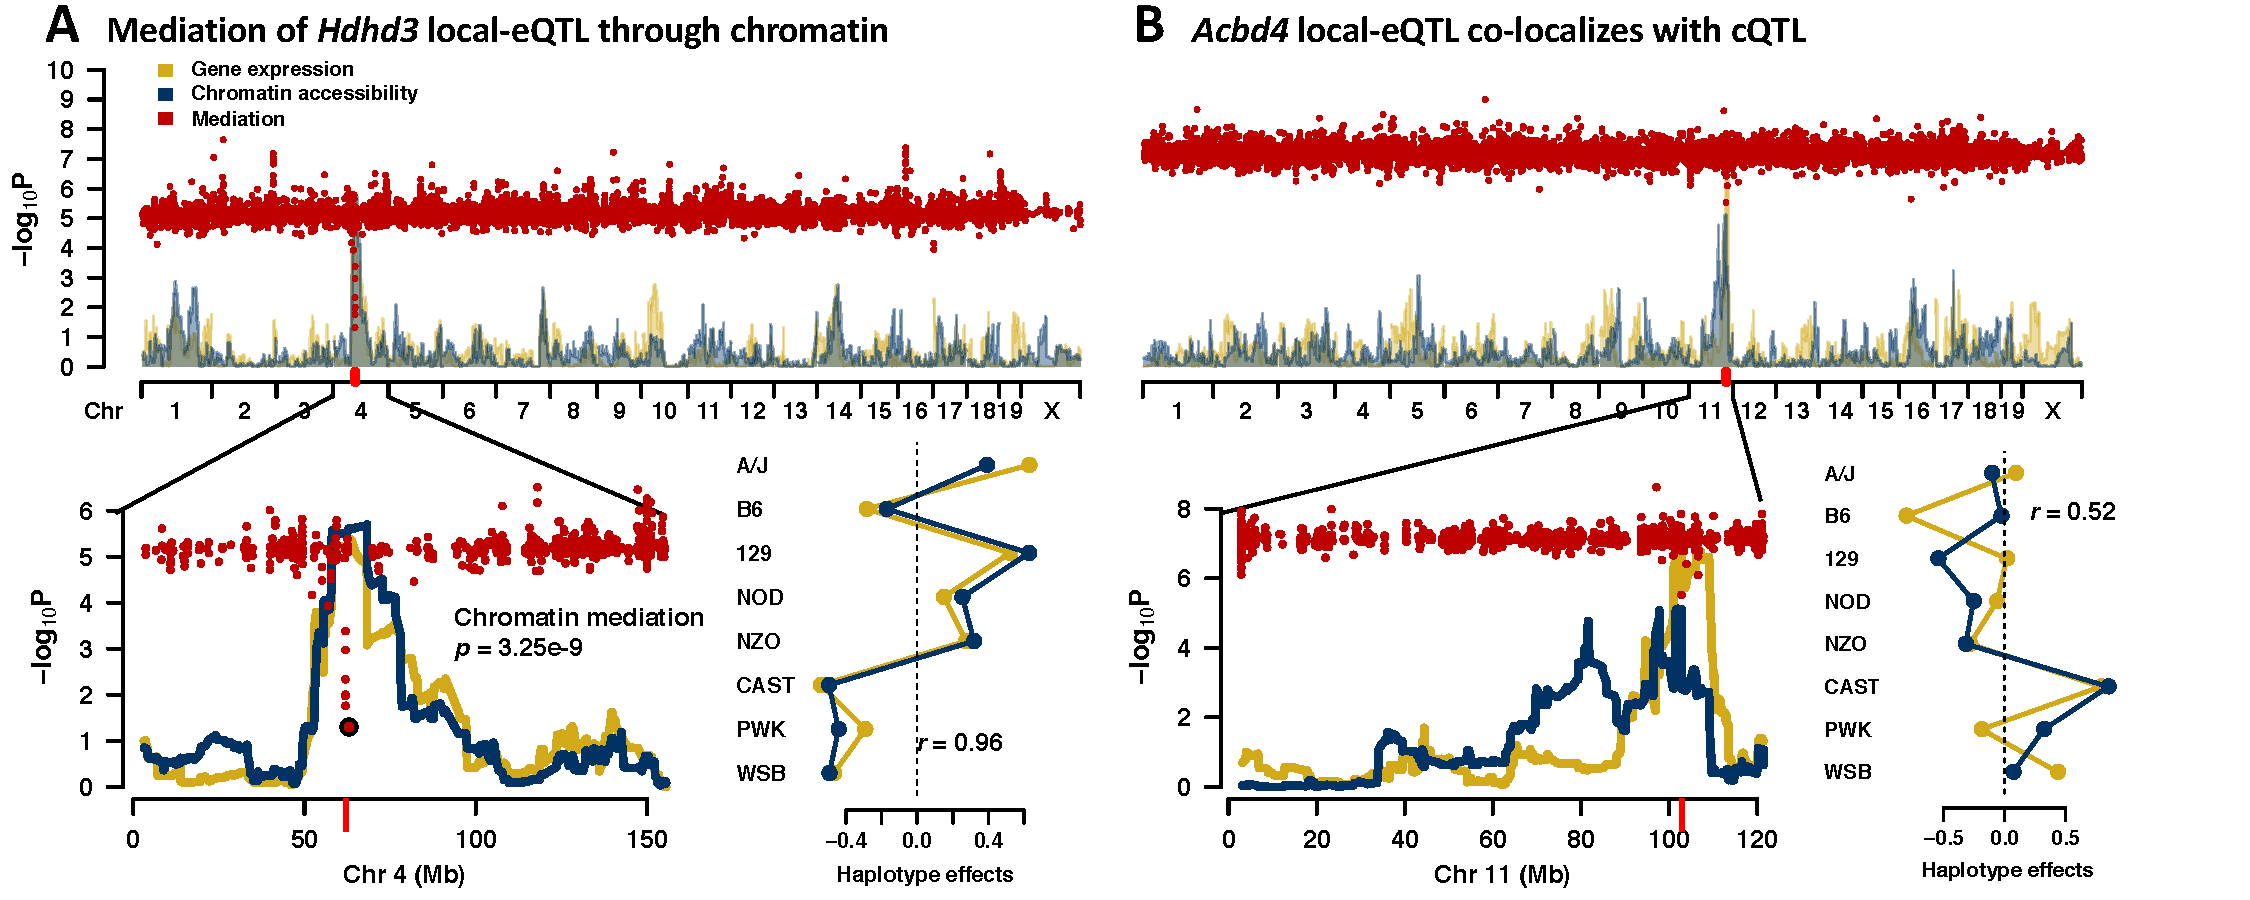
\includegraphics[width=\textwidth]{figs/mediation_or_colocal.pdf}
\caption{\textbf{Co-localizing eQTL and cQTL are not sufficient for statistical mediation.} The approach used to detect mediation through chromatin accessibility requires that the eQTL and cQTL co-localize (both within 10 Mb of the gene TSS), as well as possess similar founder allele effect patterns. Co-localizing cQTL are observed for local-eQTL for both \textit{Hdhd3} in liver \textbf{[left]} and \textit{Acbd4} in kidney \textbf{[right]}. QTL and mediation scans are included (\textbf{[top]}), with chromosomes 4 and 11 blown up for \textit{Hdhd3} and \textit{Acbd4}, respectively. The red ticks denote the TSS for both genes. The founders effects were estimated as centered and scaled BLUPs. The founder effects for the eQTL and cQTL are highly correlated ($r = 0.96$) for \textit{Hdhd3}, but not for \textit{Acbd4} ($r = 0.52$). Strong mediation of the \textit{Hdhd3} eQTL through chromatin is detected, but not for \textit{Acbd4}. The effect size of the proximal cQTL to \textit{Acbd4} is smaller than its eQTL, also inconsistent with the relationship depicted in \textbf{Figure \ref{fig:graph}[top]}.\label{fig:colocalization}}
\end{figure*}

\begin{figure*}[hp]
\renewcommand{\familydefault}{\sfdefault}\normalfont
\centering
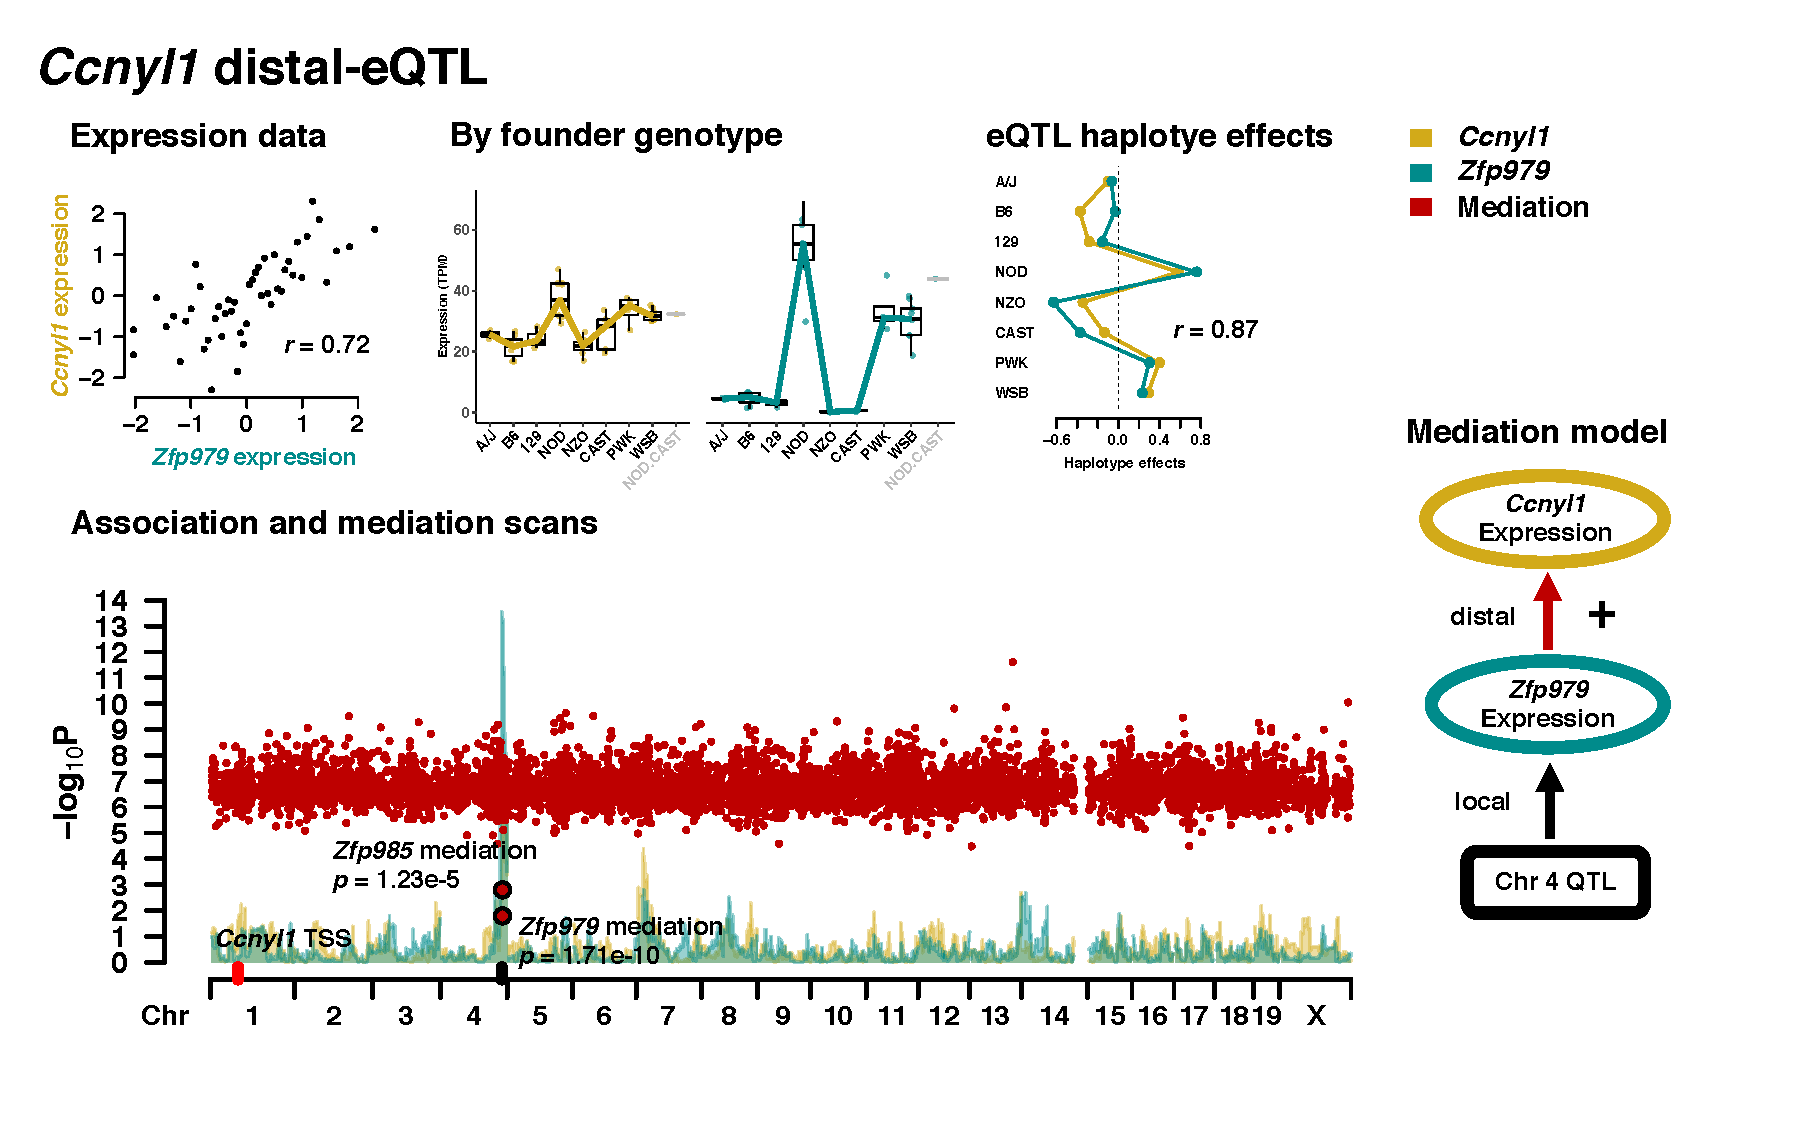
\includegraphics[width=\textwidth, trim={0in 0.5in 0in 0in}, clip]{figs/ccnyl1_mediation.pdf}
\caption{\textbf{Mediation of \textit{Ccnyl1} distal-eQTL through \textit{Zfp979} expression.} Expression of \textit{Ccnyl1} and \textit{Zfp979} are correlated ($r = 0.72$) in lung, which is also observed in the expression data categorized by diplotype and the founder effects estimated as scaled BLUPs. The distal-eQTL on chromosome 4 for \textit{Ccnyl1} corresponds closely to local-eQTL of \textit{Zfp979}. \textit{Ccnyl1} is located on chromosome 1, indicated by the red tick. \textit{Zfp979} and \textit{Zfp985}, both zinc finger proteins likely with DNA binding properties, are identified as strong candidate mediators of the distal-eQTL at genome-wide significance. The correlations, magnitude of effects, and mediation are consistent with the simple relationship depicted in the graph on the \textbf{[right]}. The distal-eQTL and candidate mediators are located in the same region of interest defined in \cite{HamiltonWilliams2013}, which also regulates \textit{Akr1e1} expression. 
\label{fig:ccnyl1_exmediation}}
\end{figure*}

\begin{figure*}[hp]
\renewcommand{\familydefault}{\sfdefault}\normalfont
\centering
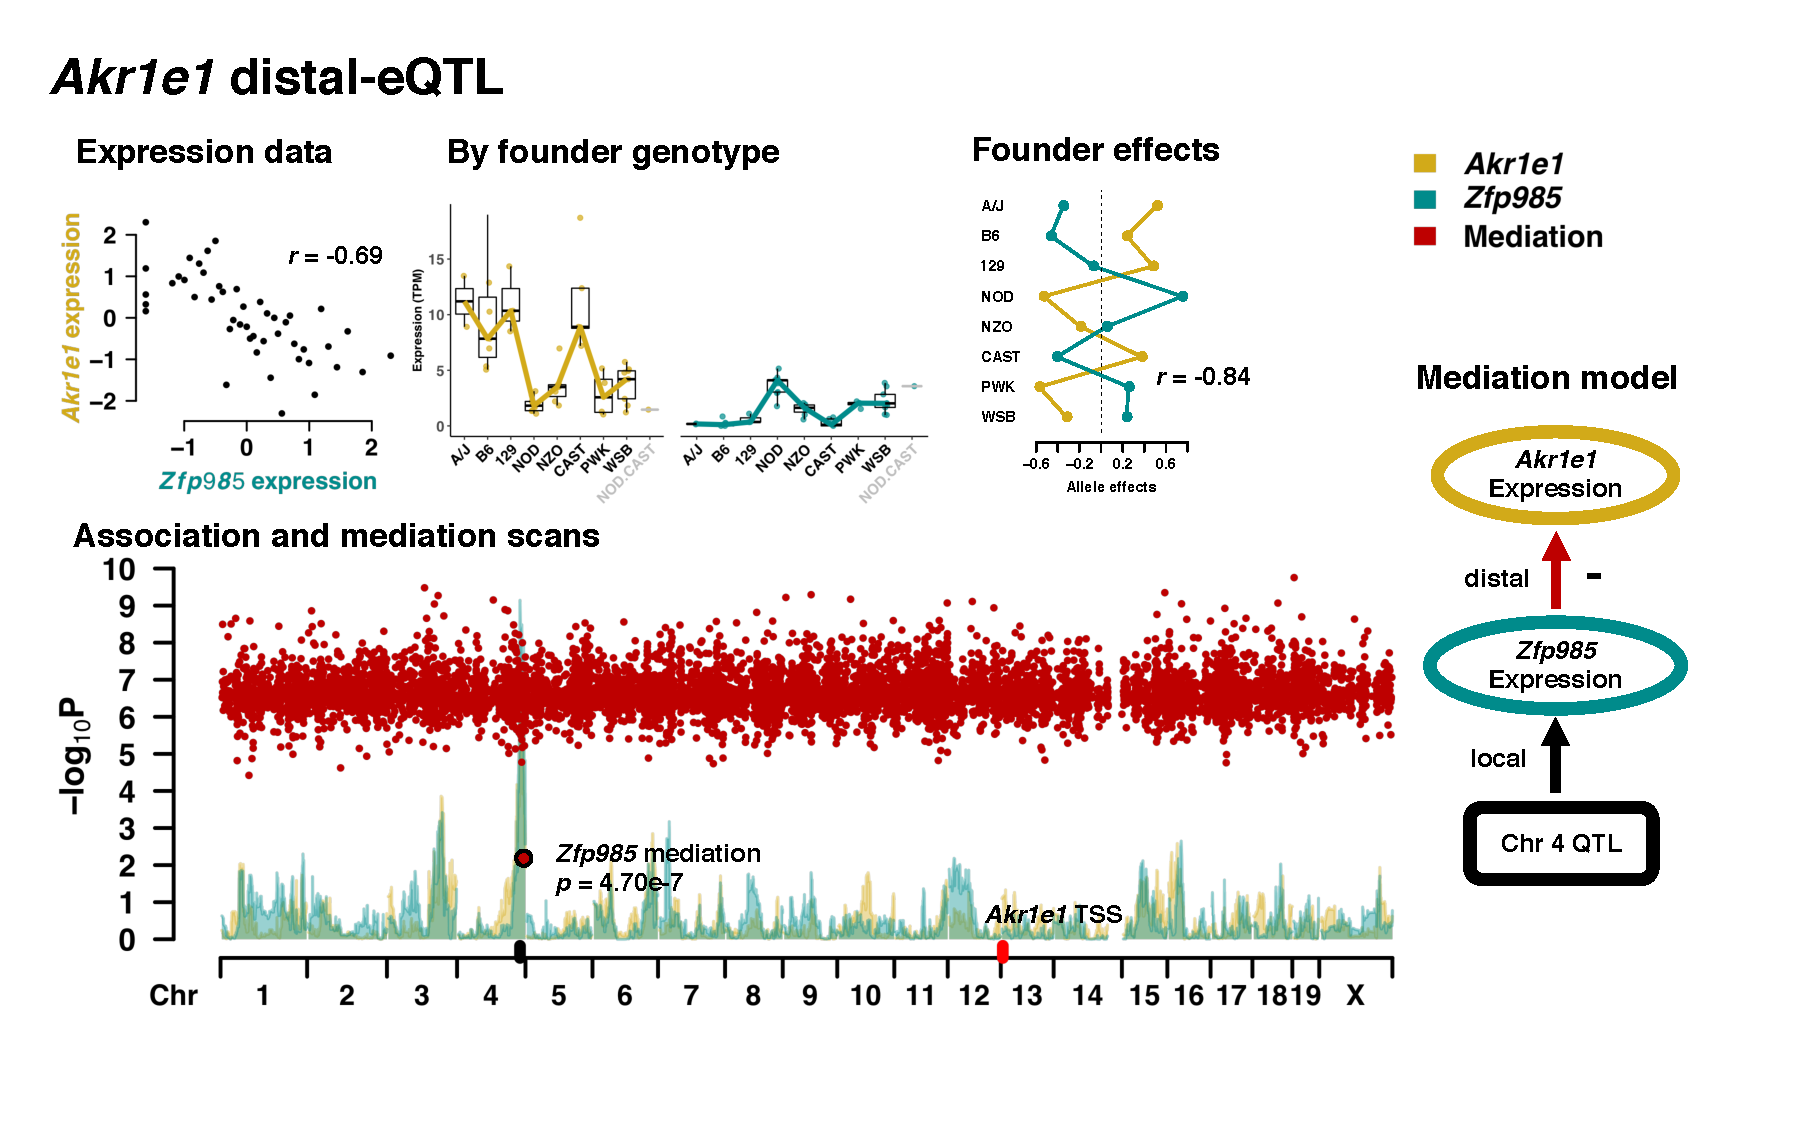
\includegraphics[width=\textwidth, trim={0in 0.5in 0in 0in}, clip]{figs/akr1e1_mediation.pdf}
\caption{\textbf{Mediation of \textit{Akr1e1} distal-eQTL through \textit{Zfp985} expression.} Expression of \textit{Akr1e1} and \textit{Zfp985} are anti-correlated ($r = -0.69$) in lung. This relationship is also observed in the expression data plotted as boxplots, categorized by most likely diplotype, and the founder allele effects, estimated as scaled BLUPs. The QTL and mediation scans reveal that \textit{Akr1e1}, TSS marked with a red tick on chromosome 13, possesses a distal-eQTL on chromosome 4 that is proximal to the strong local-eQTL of \textit{Zfp985}. The mediation scan identifies \textit{Zfp985} as a strong candidate mediator consistent with the mediation model included on the \textbf{[right]}. A more complete picture of the genetic regulation of \textit{Akr1e1} expression is pieced together by looking across all three tissues and includes a potential chromatin mediator (\textbf{Figure \ref{fig:akr1e1_full_model.pdf}}).
\label{fig:akr1e1_exmediation}}
\end{figure*}

\begin{figure*}[hp]
\renewcommand{\familydefault}{\sfdefault}\normalfont
\centering
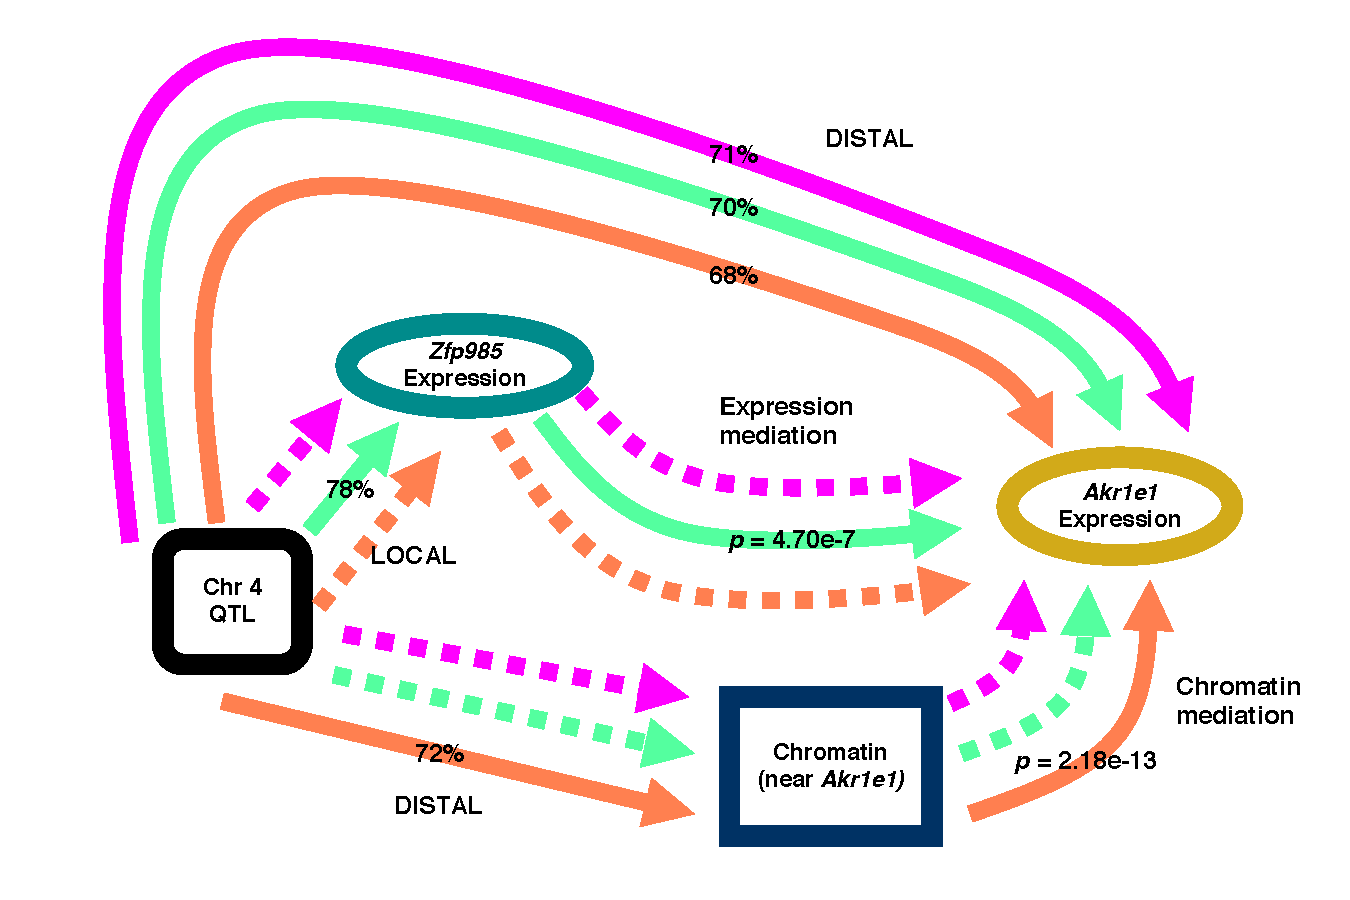
\includegraphics[width=\textwidth, trim={0in 0in 0in 0in}, clip]{figs/akr1e1_observed_relationships.pdf}
\caption{\textbf{Observed relationships across the three tissues related to the genetic regulation of \textit{Akr1e1} expression.} The model for the distal genetic regulation of \textit{Akr1e1} expression, described in \textbf{Figure \ref{fig:akr1e1_full_model}}, was reconstructed from these observed relationships. Solid arrows were observed, whereas dashed arrows are assumed. QTL effect sizes were estimated using Eq \ref{eq:effect_size}, and mediation p-values (permP) were defined using a permutation procedure. The assumed relationships are supported by the presence of the distal-eQTL in all three tissues.
\label{fig:akr1e1_relationships}}
\end{figure*}




\end{document}